\documentclass[a4paper]{book}
\usepackage{a4wide}
\usepackage{makeidx}
\usepackage{graphicx}
\usepackage{multicol}
\usepackage{float}
\usepackage{listings}
\usepackage{color}
\usepackage{textcomp}
\usepackage{alltt}
\usepackage{times}
\usepackage{ifpdf}
\ifpdf
\usepackage[pdftex,
            pagebackref=true,
            colorlinks=true,
            linkcolor=blue,
            unicode
           ]{hyperref}
\else
\usepackage[ps2pdf,
            pagebackref=true,
            colorlinks=true,
            linkcolor=blue,
            unicode
           ]{hyperref}
\usepackage{pspicture}
\fi
\usepackage[utf8]{inputenc}
\usepackage{doxygen}
\lstset{language=C++,inputencoding=utf8,basicstyle=\footnotesize,breaklines=true,breakatwhitespace=true,tabsize=4,numbers=left }
\makeindex
\setcounter{tocdepth}{3}
\renewcommand{\footrulewidth}{0.4pt}
\begin{document}
\hypersetup{pageanchor=false}
\begin{titlepage}
\vspace*{7cm}
\begin{center}
{\Large vmath \\[1ex]\large vmath-\/0.10 }\\
\vspace*{1cm}
{\large Generated by Doxygen 1.7.1}\\
\vspace*{0.5cm}
{\small Sun Nov 20 2011 20:10:09}\\
\end{center}
\end{titlepage}
\clearemptydoublepage
\pagenumbering{roman}
\tableofcontents
\clearemptydoublepage
\pagenumbering{arabic}
\hypersetup{pageanchor=true}
\chapter{Intro}
\label{index}\hypertarget{index}{}16 gid=32753351
18 uid=1520560311
20 ctime=1321817497
20 atime=1321816420
38 LIBARCHIVE.creationtime=1321815762
24 SCHILY.dev=234881029
23 SCHILY.ino=16405157
18 SCHILY.nlink=1

\chapter{License}
\label{license}
\hypertarget{license}{}
16 gid=32753351
18 uid=1520560311
20 ctime=1321817497
20 atime=1321816420
38 LIBARCHIVE.creationtime=1321815762
24 SCHILY.dev=234881029
23 SCHILY.ino=16405156
18 SCHILY.nlink=1

\chapter{Class Index}
16 gid=32753351
18 uid=1520560311
20 ctime=1321817497
20 atime=1321816420
38 LIBARCHIVE.creationtime=1321815762
24 SCHILY.dev=234881029
23 SCHILY.ino=16405141
18 SCHILY.nlink=1

\chapter{File Index}
\section{File List}
Here is a list of all files with brief descriptions:\begin{DoxyCompactList}
\item\contentsline{section}{src/\hyperlink{vmath_8cpp}{vmath.cpp} }{\pageref{vmath_8cpp}}{}
\item\contentsline{section}{src/\hyperlink{vmath_8h}{vmath.h} }{\pageref{vmath_8h}}{}
\end{DoxyCompactList}

\chapter{Class Documentation}
\hypertarget{class_matrix3}{
\section{Matrix3$<$ T $>$ Class Template Reference}
\label{class_matrix3}\index{Matrix3@{Matrix3}}
}


Class for matrix 3x3.  




{\ttfamily \#include $<$vmath.h$>$}



Collaboration diagram for Matrix3$<$ T $>$:
\nopagebreak
\begin{figure}[H]
\begin{center}
\leavevmode
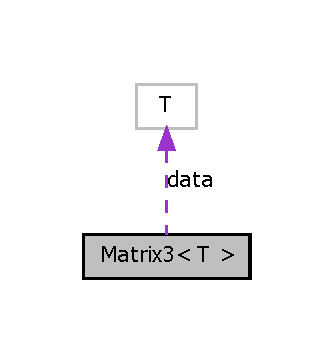
\includegraphics[width=160pt]{class_matrix3__coll__graph}
\end{center}
\end{figure}
\subsection*{Public Member Functions}
\begin{DoxyCompactItemize}
\item 
\hyperlink{class_matrix3_afbc8b655540e4b5b04d8439b606303b0}{Matrix3} ()
\begin{DoxyCompactList}\small\item\em Creates identity matrix. \item\end{DoxyCompactList}\item 
\hyperlink{class_matrix3_a3986b8f36efefb3ab2455e86fdb5e327}{Matrix3} (const T $\ast$dt)
\begin{DoxyCompactList}\small\item\em Copy matrix values from array (these data must be in column major order!). \item\end{DoxyCompactList}\item 
\hyperlink{class_matrix3_a7f0b1ceaedeffd2ab458b6dc7edc358c}{Matrix3} (const \hyperlink{class_matrix3}{Matrix3}$<$ T $>$ \&src)
\begin{DoxyCompactList}\small\item\em Copy constructor. \item\end{DoxyCompactList}\item 
{\footnotesize template$<$class FromT $>$ }\\\hyperlink{class_matrix3_acf94796374f73b4559336f08e233038c}{Matrix3} (const \hyperlink{class_matrix3}{Matrix3}$<$ FromT $>$ \&src)
\begin{DoxyCompactList}\small\item\em Copy casting constructor. \item\end{DoxyCompactList}\item 
void \hyperlink{class_matrix3_a44360e8ae549ec4b2b9c0f8ed4786761}{identity} ()
\begin{DoxyCompactList}\small\item\em Resets matrix to be identity matrix. \item\end{DoxyCompactList}\item 
bool \hyperlink{class_matrix3_acf8dc6060016d09250b8706e89f4dcc0}{operator==} (const \hyperlink{class_matrix3}{Matrix3}$<$ T $>$ \&rhs) const 
\begin{DoxyCompactList}\small\item\em Equality test operator. \item\end{DoxyCompactList}\item 
bool \hyperlink{class_matrix3_a1ecdce469f979786b1fa257a6fca3866}{operator!=} (const \hyperlink{class_matrix3}{Matrix3}$<$ T $>$ \&rhs) const 
\begin{DoxyCompactList}\small\item\em Inequality test operator. \item\end{DoxyCompactList}\item 
T \& \hyperlink{class_matrix3_aba232062fee5e35419c2c0c73aa9b88d}{at} (int x, int y)
\begin{DoxyCompactList}\small\item\em Get reference to element at position (x,y). \item\end{DoxyCompactList}\item 
const T \& \hyperlink{class_matrix3_abd32ca6519bd0131709cdeca665b4a23}{at} (int x, int y) const 
\begin{DoxyCompactList}\small\item\em Get constant reference to element at position (x,y). \item\end{DoxyCompactList}\item 
T \& \hyperlink{class_matrix3_a21a0e224becfb4fa4447d4c656ad3d0c}{operator()} (int i, int j)
\begin{DoxyCompactList}\small\item\em Get reference to element at position (i,j), with math matrix notation. \item\end{DoxyCompactList}\item 
const T \& \hyperlink{class_matrix3_a345b3ea5baef035e1272506540c2905c}{operator()} (int i, int j) const 
\begin{DoxyCompactList}\small\item\em Get constant reference to element at position (i,j), with math matrix notation. \item\end{DoxyCompactList}\item 
\hyperlink{class_matrix3}{Matrix3}$<$ T $>$ \& \hyperlink{class_matrix3_afcd3742e1bb4ce693fd28c751a4d8e9c}{operator=} (const \hyperlink{class_matrix3}{Matrix3}$<$ T $>$ \&rhs)
\begin{DoxyCompactList}\small\item\em Copy operator. \item\end{DoxyCompactList}\item 
{\footnotesize template$<$class FromT $>$ }\\\hyperlink{class_matrix3}{Matrix3}$<$ T $>$ \& \hyperlink{class_matrix3_a8fc1aae99bf569de84249e8716ce50e8}{operator=} (const \hyperlink{class_matrix3}{Matrix3}$<$ FromT $>$ \&rhs)
\begin{DoxyCompactList}\small\item\em Copy casting operator. \item\end{DoxyCompactList}\item 
\hyperlink{class_matrix3}{Matrix3}$<$ T $>$ \& \hyperlink{class_matrix3_a0c34f193be3802cae81c4cbfdfab1a53}{operator=} (const T $\ast$rhs)
\begin{DoxyCompactList}\small\item\em Copy operator. \item\end{DoxyCompactList}\item 
\hyperlink{class_matrix3}{Matrix3}$<$ T $>$ \hyperlink{class_matrix3_ad960991a64a1e6c72e21c29fb8c1f890}{operator+} (const \hyperlink{class_matrix3}{Matrix3}$<$ T $>$ \&rhs) const 
\begin{DoxyCompactList}\small\item\em Addition operator. \item\end{DoxyCompactList}\item 
\hyperlink{class_matrix3}{Matrix3}$<$ T $>$ \hyperlink{class_matrix3_aeb5ca229fa633ceec14fc93fa873234d}{operator-\/} (const \hyperlink{class_matrix3}{Matrix3}$<$ T $>$ \&rhs) const 
\begin{DoxyCompactList}\small\item\em Subtraction operator. \item\end{DoxyCompactList}\item 
\hyperlink{class_matrix3}{Matrix3}$<$ T $>$ \hyperlink{class_matrix3_a635803865b0b5c3c0e2102a44d7ed5d8}{operator+} (T rhs) const 
\begin{DoxyCompactList}\small\item\em Addition operator. \item\end{DoxyCompactList}\item 
\hyperlink{class_matrix3}{Matrix3}$<$ T $>$ \hyperlink{class_matrix3_a708ee4b7775f551c63e1d1820ef1d7b2}{operator-\/} (T rhs) const 
\begin{DoxyCompactList}\small\item\em Subtraction operator. \item\end{DoxyCompactList}\item 
\hyperlink{class_matrix3}{Matrix3}$<$ T $>$ \hyperlink{class_matrix3_a4a7053f22eee3c50ef099181983370c9}{operator$\ast$} (T rhs) const 
\begin{DoxyCompactList}\small\item\em Multiplication operator. \item\end{DoxyCompactList}\item 
\hyperlink{class_matrix3}{Matrix3}$<$ T $>$ \hyperlink{class_matrix3_abf53af4ad067516b153c76a9e18cc410}{operator/} (T rhs) const 
\begin{DoxyCompactList}\small\item\em Division operator. \item\end{DoxyCompactList}\item 
\hyperlink{class_vector3}{Vector3}$<$ T $>$ \hyperlink{class_matrix3_add25a42745c41871b2d3b808f0d5047e}{operator$\ast$} (const \hyperlink{class_vector3}{Vector3}$<$ T $>$ \&rhs) const 
\begin{DoxyCompactList}\small\item\em Multiplication operator. \item\end{DoxyCompactList}\item 
\hyperlink{class_matrix3}{Matrix3}$<$ T $>$ \hyperlink{class_matrix3_abd84667793375507dc98fc8e896d89b3}{operator$\ast$} (\hyperlink{class_matrix3}{Matrix3}$<$ T $>$ rhs) const 
\begin{DoxyCompactList}\small\item\em Multiplication operator. \item\end{DoxyCompactList}\item 
\hyperlink{class_matrix3}{Matrix3}$<$ T $>$ \hyperlink{class_matrix3_aafac87a5bb5afd70a7a8b39257f28558}{transpose} ()
\begin{DoxyCompactList}\small\item\em Transpose matrix. \item\end{DoxyCompactList}\item 
\hyperlink{class_matrix3}{Matrix3}$<$ T $>$ \hyperlink{class_matrix3_a3c16292eeaf2514a4fc26de912cf07e0}{lerp} (T fact, const \hyperlink{class_matrix3}{Matrix3}$<$ T $>$ \&rhs) const 
\begin{DoxyCompactList}\small\item\em Linear interpolation of two matrices. \item\end{DoxyCompactList}\item 
T \hyperlink{class_matrix3_a4cba34533d0f88feb8a622e5c5b7052d}{det} ()
\item 
\hyperlink{class_matrix3}{Matrix3}$<$ T $>$ \hyperlink{class_matrix3_aad3810622196a42d5f1a58e7d49d1417}{inverse} ()
\begin{DoxyCompactList}\small\item\em Computes inverse matrix. \item\end{DoxyCompactList}\item 
\hyperlink{class_matrix3_a643aecc11c95f9706a7620deab32a4ee}{operator T $\ast$} ()
\begin{DoxyCompactList}\small\item\em Conversion to pointer operator. \item\end{DoxyCompactList}\item 
\hyperlink{class_matrix3_a103a13ad3c2c32985e6e10adb91088f2}{operator const T $\ast$} () const 
\begin{DoxyCompactList}\small\item\em Conversion to pointer operator. \item\end{DoxyCompactList}\item 
std::string \hyperlink{class_matrix3_a4208a1713fc7fb654a88eb7b82ef3b02}{toString} () const 
\begin{DoxyCompactList}\small\item\em Gets string representation. \item\end{DoxyCompactList}\end{DoxyCompactItemize}
\subsection*{Static Public Member Functions}
\begin{DoxyCompactItemize}
\item 
static \hyperlink{class_matrix3}{Matrix3}$<$ T $>$ \hyperlink{class_matrix3_a1e39496a1d1708ddc1658b0bf2f448f2}{createRotationAroundAxis} (T xDeg, T yDeg, T zDeg)
\begin{DoxyCompactList}\small\item\em Creates rotation matrix by rotation around axis. \item\end{DoxyCompactList}\item 
{\footnotesize template$<$class It $>$ }\\static \hyperlink{class_matrix3}{Matrix3}$<$ T $>$ \hyperlink{class_matrix3_af183cabaf18b9922fd11e517c5cf26b1}{fromOde} (const It $\ast$mat)
\begin{DoxyCompactList}\small\item\em Creates rotation matrix from ODE Matrix. \item\end{DoxyCompactList}\item 
{\footnotesize template$<$class FromT $>$ }\\static \hyperlink{class_matrix3}{Matrix3}$<$ T $>$ \hyperlink{class_matrix3_abce4ed104a81e64ce9cbd479f0105625}{fromRowMajorArray} (const FromT $\ast$arr)
\begin{DoxyCompactList}\small\item\em Creates new matrix 3x3 from array that represents such matrix 3x3 as array of tightly packed elements in row major order. \item\end{DoxyCompactList}\item 
{\footnotesize template$<$class FromT $>$ }\\static \hyperlink{class_matrix3}{Matrix3}$<$ T $>$ \hyperlink{class_matrix3_a54ac5b79264837228f219067e92aa853}{fromColumnMajorArray} (const FromT $\ast$arr)
\begin{DoxyCompactList}\small\item\em Creates new matrix 3x3 from array that represents such matrix 3x3 as array of tightly packed elements in column major order. \item\end{DoxyCompactList}\end{DoxyCompactItemize}
\subsection*{Public Attributes}
\begin{DoxyCompactItemize}
\item 
T \hyperlink{class_matrix3_ad0e5ea83502126b24d468ae8cc67255d}{data} \mbox{[}9\mbox{]}
\begin{DoxyCompactList}\small\item\em Data stored in column major order. \item\end{DoxyCompactList}\end{DoxyCompactItemize}
\subsection*{Friends}
\begin{DoxyCompactItemize}
\item 
std::ostream \& \hyperlink{class_matrix3_a281742a1b77b4a4bf76ac03f7b75ee74}{operator$<$$<$} (std::ostream \&lhs, const \hyperlink{class_matrix3}{Matrix3}$<$ T $>$ \&rhs)
\begin{DoxyCompactList}\small\item\em Output to stream operator. \item\end{DoxyCompactList}\end{DoxyCompactItemize}


\subsection{Detailed Description}
\subsubsection*{template$<$class T$>$ class Matrix3$<$ T $>$}

Class for matrix 3x3. \begin{DoxyNote}{Note}
Data stored in this matrix are in column major order. This arrangement suits OpenGL. If you're using row major matrix, consider using fromRowMajorArray as way for construction Matrix3$<$T$>$ instance. 
\end{DoxyNote}


\subsection{Constructor \& Destructor Documentation}
\hypertarget{class_matrix3_afbc8b655540e4b5b04d8439b606303b0}{
\index{Matrix3@{Matrix3}!Matrix3@{Matrix3}}
\index{Matrix3@{Matrix3}!Matrix3@{Matrix3}}
\subsubsection[{Matrix3}]{\setlength{\rightskip}{0pt plus 5cm}template$<$class T$>$ {\bf Matrix3}$<$ T $>$::{\bf Matrix3} (
\begin{DoxyParamCaption}
{}
\end{DoxyParamCaption}
)\hspace{0.3cm}{\ttfamily  \mbox{[}inline\mbox{]}}}}
\label{class_matrix3_afbc8b655540e4b5b04d8439b606303b0}


Creates identity matrix. 

\hypertarget{class_matrix3_a3986b8f36efefb3ab2455e86fdb5e327}{
\index{Matrix3@{Matrix3}!Matrix3@{Matrix3}}
\index{Matrix3@{Matrix3}!Matrix3@{Matrix3}}
\subsubsection[{Matrix3}]{\setlength{\rightskip}{0pt plus 5cm}template$<$class T$>$ {\bf Matrix3}$<$ T $>$::{\bf Matrix3} (
\begin{DoxyParamCaption}
\item[{const T $\ast$}]{ dt}
\end{DoxyParamCaption}
)\hspace{0.3cm}{\ttfamily  \mbox{[}inline\mbox{]}}}}
\label{class_matrix3_a3986b8f36efefb3ab2455e86fdb5e327}


Copy matrix values from array (these data must be in column major order!). 

\hypertarget{class_matrix3_a7f0b1ceaedeffd2ab458b6dc7edc358c}{
\index{Matrix3@{Matrix3}!Matrix3@{Matrix3}}
\index{Matrix3@{Matrix3}!Matrix3@{Matrix3}}
\subsubsection[{Matrix3}]{\setlength{\rightskip}{0pt plus 5cm}template$<$class T$>$ {\bf Matrix3}$<$ T $>$::{\bf Matrix3} (
\begin{DoxyParamCaption}
\item[{const {\bf Matrix3}$<$ T $>$ \&}]{ src}
\end{DoxyParamCaption}
)\hspace{0.3cm}{\ttfamily  \mbox{[}inline\mbox{]}}}}
\label{class_matrix3_a7f0b1ceaedeffd2ab458b6dc7edc358c}


Copy constructor. 


\begin{DoxyParams}{Parameters}
\item[{\em src}]Data source for new created instance of \hyperlink{class_matrix3}{Matrix3} \end{DoxyParams}
\hypertarget{class_matrix3_acf94796374f73b4559336f08e233038c}{
\index{Matrix3@{Matrix3}!Matrix3@{Matrix3}}
\index{Matrix3@{Matrix3}!Matrix3@{Matrix3}}
\subsubsection[{Matrix3}]{\setlength{\rightskip}{0pt plus 5cm}template$<$class T$>$ template$<$class FromT $>$ {\bf Matrix3}$<$ T $>$::{\bf Matrix3} (
\begin{DoxyParamCaption}
\item[{const {\bf Matrix3}$<$ FromT $>$ \&}]{ src}
\end{DoxyParamCaption}
)\hspace{0.3cm}{\ttfamily  \mbox{[}inline\mbox{]}}}}
\label{class_matrix3_acf94796374f73b4559336f08e233038c}


Copy casting constructor. 


\begin{DoxyParams}{Parameters}
\item[{\em src}]Data source for new created instance of \hyperlink{class_matrix3}{Matrix3} \end{DoxyParams}


\subsection{Member Function Documentation}
\hypertarget{class_matrix3_aba232062fee5e35419c2c0c73aa9b88d}{
\index{Matrix3@{Matrix3}!at@{at}}
\index{at@{at}!Matrix3@{Matrix3}}
\subsubsection[{at}]{\setlength{\rightskip}{0pt plus 5cm}template$<$class T$>$ T\& {\bf Matrix3}$<$ T $>$::at (
\begin{DoxyParamCaption}
\item[{int}]{ x, }
\item[{int}]{ y}
\end{DoxyParamCaption}
)\hspace{0.3cm}{\ttfamily  \mbox{[}inline\mbox{]}}}}
\label{class_matrix3_aba232062fee5e35419c2c0c73aa9b88d}


Get reference to element at position (x,y). 


\begin{DoxyParams}{Parameters}
\item[{\em x}]Number of column (0..2) \item[{\em y}]Number of row (0..2) \end{DoxyParams}
\hypertarget{class_matrix3_abd32ca6519bd0131709cdeca665b4a23}{
\index{Matrix3@{Matrix3}!at@{at}}
\index{at@{at}!Matrix3@{Matrix3}}
\subsubsection[{at}]{\setlength{\rightskip}{0pt plus 5cm}template$<$class T$>$ const T\& {\bf Matrix3}$<$ T $>$::at (
\begin{DoxyParamCaption}
\item[{int}]{ x, }
\item[{int}]{ y}
\end{DoxyParamCaption}
) const\hspace{0.3cm}{\ttfamily  \mbox{[}inline\mbox{]}}}}
\label{class_matrix3_abd32ca6519bd0131709cdeca665b4a23}


Get constant reference to element at position (x,y). 


\begin{DoxyParams}{Parameters}
\item[{\em x}]Number of column (0..2) \item[{\em y}]Number of row (0..2) \end{DoxyParams}
\hypertarget{class_matrix3_a1e39496a1d1708ddc1658b0bf2f448f2}{
\index{Matrix3@{Matrix3}!createRotationAroundAxis@{createRotationAroundAxis}}
\index{createRotationAroundAxis@{createRotationAroundAxis}!Matrix3@{Matrix3}}
\subsubsection[{createRotationAroundAxis}]{\setlength{\rightskip}{0pt plus 5cm}template$<$class T$>$ static {\bf Matrix3}$<$T$>$ {\bf Matrix3}$<$ T $>$::createRotationAroundAxis (
\begin{DoxyParamCaption}
\item[{T}]{ xDeg, }
\item[{T}]{ yDeg, }
\item[{T}]{ zDeg}
\end{DoxyParamCaption}
)\hspace{0.3cm}{\ttfamily  \mbox{[}inline, static\mbox{]}}}}
\label{class_matrix3_a1e39496a1d1708ddc1658b0bf2f448f2}


Creates rotation matrix by rotation around axis. 


\begin{DoxyParams}{Parameters}
\item[{\em xDeg}]Angle (in degrees) of rotation around axis X. \item[{\em yDeg}]Angle (in degrees) of rotation around axis Y. \item[{\em zDeg}]Angle (in degrees) of rotation around axis Z. \end{DoxyParams}
\hypertarget{class_matrix3_a4cba34533d0f88feb8a622e5c5b7052d}{
\index{Matrix3@{Matrix3}!det@{det}}
\index{det@{det}!Matrix3@{Matrix3}}
\subsubsection[{det}]{\setlength{\rightskip}{0pt plus 5cm}template$<$class T$>$ T {\bf Matrix3}$<$ T $>$::det (
\begin{DoxyParamCaption}
{}
\end{DoxyParamCaption}
)\hspace{0.3cm}{\ttfamily  \mbox{[}inline\mbox{]}}}}
\label{class_matrix3_a4cba34533d0f88feb8a622e5c5b7052d}
\hypertarget{class_matrix3_a54ac5b79264837228f219067e92aa853}{
\index{Matrix3@{Matrix3}!fromColumnMajorArray@{fromColumnMajorArray}}
\index{fromColumnMajorArray@{fromColumnMajorArray}!Matrix3@{Matrix3}}
\subsubsection[{fromColumnMajorArray}]{\setlength{\rightskip}{0pt plus 5cm}template$<$class T$>$ template$<$class FromT $>$ static {\bf Matrix3}$<$T$>$ {\bf Matrix3}$<$ T $>$::fromColumnMajorArray (
\begin{DoxyParamCaption}
\item[{const FromT $\ast$}]{ arr}
\end{DoxyParamCaption}
)\hspace{0.3cm}{\ttfamily  \mbox{[}inline, static\mbox{]}}}}
\label{class_matrix3_a54ac5b79264837228f219067e92aa853}


Creates new matrix 3x3 from array that represents such matrix 3x3 as array of tightly packed elements in column major order. 


\begin{DoxyParams}{Parameters}
\item[{\em arr}]An array of elements for 3x3 matrix in column major order. \end{DoxyParams}
\begin{DoxyReturn}{Returns}
An instance of Matrix3$<$T$>$ representing {\itshape arr\/} 
\end{DoxyReturn}
\hypertarget{class_matrix3_af183cabaf18b9922fd11e517c5cf26b1}{
\index{Matrix3@{Matrix3}!fromOde@{fromOde}}
\index{fromOde@{fromOde}!Matrix3@{Matrix3}}
\subsubsection[{fromOde}]{\setlength{\rightskip}{0pt plus 5cm}template$<$class T$>$ template$<$class It $>$ static {\bf Matrix3}$<$T$>$ {\bf Matrix3}$<$ T $>$::fromOde (
\begin{DoxyParamCaption}
\item[{const It $\ast$}]{ mat}
\end{DoxyParamCaption}
)\hspace{0.3cm}{\ttfamily  \mbox{[}inline, static\mbox{]}}}}
\label{class_matrix3_af183cabaf18b9922fd11e517c5cf26b1}


Creates rotation matrix from ODE Matrix. 

\hypertarget{class_matrix3_abce4ed104a81e64ce9cbd479f0105625}{
\index{Matrix3@{Matrix3}!fromRowMajorArray@{fromRowMajorArray}}
\index{fromRowMajorArray@{fromRowMajorArray}!Matrix3@{Matrix3}}
\subsubsection[{fromRowMajorArray}]{\setlength{\rightskip}{0pt plus 5cm}template$<$class T$>$ template$<$class FromT $>$ static {\bf Matrix3}$<$T$>$ {\bf Matrix3}$<$ T $>$::fromRowMajorArray (
\begin{DoxyParamCaption}
\item[{const FromT $\ast$}]{ arr}
\end{DoxyParamCaption}
)\hspace{0.3cm}{\ttfamily  \mbox{[}inline, static\mbox{]}}}}
\label{class_matrix3_abce4ed104a81e64ce9cbd479f0105625}


Creates new matrix 3x3 from array that represents such matrix 3x3 as array of tightly packed elements in row major order. 


\begin{DoxyParams}{Parameters}
\item[{\em arr}]An array of elements for 3x3 matrix in row major order. \end{DoxyParams}
\begin{DoxyReturn}{Returns}
An instance of Matrix3$<$T$>$ representing {\itshape arr\/} 
\end{DoxyReturn}
\hypertarget{class_matrix3_a44360e8ae549ec4b2b9c0f8ed4786761}{
\index{Matrix3@{Matrix3}!identity@{identity}}
\index{identity@{identity}!Matrix3@{Matrix3}}
\subsubsection[{identity}]{\setlength{\rightskip}{0pt plus 5cm}template$<$class T$>$ void {\bf Matrix3}$<$ T $>$::identity (
\begin{DoxyParamCaption}
{}
\end{DoxyParamCaption}
)\hspace{0.3cm}{\ttfamily  \mbox{[}inline\mbox{]}}}}
\label{class_matrix3_a44360e8ae549ec4b2b9c0f8ed4786761}


Resets matrix to be identity matrix. 

\hypertarget{class_matrix3_aad3810622196a42d5f1a58e7d49d1417}{
\index{Matrix3@{Matrix3}!inverse@{inverse}}
\index{inverse@{inverse}!Matrix3@{Matrix3}}
\subsubsection[{inverse}]{\setlength{\rightskip}{0pt plus 5cm}template$<$class T$>$ {\bf Matrix3}$<$T$>$ {\bf Matrix3}$<$ T $>$::inverse (
\begin{DoxyParamCaption}
{}
\end{DoxyParamCaption}
)\hspace{0.3cm}{\ttfamily  \mbox{[}inline\mbox{]}}}}
\label{class_matrix3_aad3810622196a42d5f1a58e7d49d1417}


Computes inverse matrix. 

\begin{DoxyReturn}{Returns}
Inverse matrix of this matrix. 
\end{DoxyReturn}
\hypertarget{class_matrix3_a3c16292eeaf2514a4fc26de912cf07e0}{
\index{Matrix3@{Matrix3}!lerp@{lerp}}
\index{lerp@{lerp}!Matrix3@{Matrix3}}
\subsubsection[{lerp}]{\setlength{\rightskip}{0pt plus 5cm}template$<$class T$>$ {\bf Matrix3}$<$T$>$ {\bf Matrix3}$<$ T $>$::lerp (
\begin{DoxyParamCaption}
\item[{T}]{ fact, }
\item[{const {\bf Matrix3}$<$ T $>$ \&}]{ rhs}
\end{DoxyParamCaption}
) const\hspace{0.3cm}{\ttfamily  \mbox{[}inline\mbox{]}}}}
\label{class_matrix3_a3c16292eeaf2514a4fc26de912cf07e0}


Linear interpolation of two matrices. 


\begin{DoxyParams}{Parameters}
\item[{\em fact}]Factor of interpolation. For translation from positon of this matrix (lhs) to matrix rhs, values of factor goes from 0.0 to 1.0. \item[{\em rhs}]Second Matrix for interpolation \end{DoxyParams}
\begin{DoxyNote}{Note}
However values of fact parameter are reasonable only in interval \mbox{[}0.0 , 1.0\mbox{]}, you can pass also values outside of this interval and you can get result (extrapolation?) 
\end{DoxyNote}
\hypertarget{class_matrix3_a103a13ad3c2c32985e6e10adb91088f2}{
\index{Matrix3@{Matrix3}!operator const T $\ast$@{operator const T $\ast$}}
\index{operator const T $\ast$@{operator const T $\ast$}!Matrix3@{Matrix3}}
\subsubsection[{operator const T $\ast$}]{\setlength{\rightskip}{0pt plus 5cm}template$<$class T$>$ {\bf Matrix3}$<$ T $>$::operator const T $\ast$ (
\begin{DoxyParamCaption}
{}
\end{DoxyParamCaption}
) const\hspace{0.3cm}{\ttfamily  \mbox{[}inline\mbox{]}}}}
\label{class_matrix3_a103a13ad3c2c32985e6e10adb91088f2}


Conversion to pointer operator. 

\begin{DoxyReturn}{Returns}
Constant Pointer to internally stored (in management of class Matrix3$<$T$>$) used for passing Matrix3$<$T$>$ values to gl$\ast$\mbox{[}fd\mbox{]}v functions. 
\end{DoxyReturn}
\hypertarget{class_matrix3_a643aecc11c95f9706a7620deab32a4ee}{
\index{Matrix3@{Matrix3}!operator T $\ast$@{operator T $\ast$}}
\index{operator T $\ast$@{operator T $\ast$}!Matrix3@{Matrix3}}
\subsubsection[{operator T $\ast$}]{\setlength{\rightskip}{0pt plus 5cm}template$<$class T$>$ {\bf Matrix3}$<$ T $>$::operator T $\ast$ (
\begin{DoxyParamCaption}
{}
\end{DoxyParamCaption}
)\hspace{0.3cm}{\ttfamily  \mbox{[}inline\mbox{]}}}}
\label{class_matrix3_a643aecc11c95f9706a7620deab32a4ee}


Conversion to pointer operator. 

\begin{DoxyReturn}{Returns}
Pointer to internally stored (in management of class Matrix3$<$T$>$) used for passing Matrix3$<$T$>$ values to gl$\ast$\mbox{[}fd\mbox{]}v functions. 
\end{DoxyReturn}
\hypertarget{class_matrix3_a1ecdce469f979786b1fa257a6fca3866}{
\index{Matrix3@{Matrix3}!operator!=@{operator!=}}
\index{operator!=@{operator!=}!Matrix3@{Matrix3}}
\subsubsection[{operator!=}]{\setlength{\rightskip}{0pt plus 5cm}template$<$class T$>$ bool {\bf Matrix3}$<$ T $>$::operator!= (
\begin{DoxyParamCaption}
\item[{const {\bf Matrix3}$<$ T $>$ \&}]{ rhs}
\end{DoxyParamCaption}
) const\hspace{0.3cm}{\ttfamily  \mbox{[}inline\mbox{]}}}}
\label{class_matrix3_a1ecdce469f979786b1fa257a6fca3866}


Inequality test operator. 


\begin{DoxyParams}{Parameters}
\item[{\em rhs}]Right hand side argument of binary operator. \end{DoxyParams}
\begin{DoxyReturn}{Returns}
not (lhs == rhs) :-\/P 
\end{DoxyReturn}
\hypertarget{class_matrix3_a21a0e224becfb4fa4447d4c656ad3d0c}{
\index{Matrix3@{Matrix3}!operator()@{operator()}}
\index{operator()@{operator()}!Matrix3@{Matrix3}}
\subsubsection[{operator()}]{\setlength{\rightskip}{0pt plus 5cm}template$<$class T$>$ T\& {\bf Matrix3}$<$ T $>$::operator() (
\begin{DoxyParamCaption}
\item[{int}]{ i, }
\item[{int}]{ j}
\end{DoxyParamCaption}
)\hspace{0.3cm}{\ttfamily  \mbox{[}inline\mbox{]}}}}
\label{class_matrix3_a21a0e224becfb4fa4447d4c656ad3d0c}


Get reference to element at position (i,j), with math matrix notation. 


\begin{DoxyParams}{Parameters}
\item[{\em i}]Number of row (1..3) \item[{\em j}]Number of column (1..3) \end{DoxyParams}
\hypertarget{class_matrix3_a345b3ea5baef035e1272506540c2905c}{
\index{Matrix3@{Matrix3}!operator()@{operator()}}
\index{operator()@{operator()}!Matrix3@{Matrix3}}
\subsubsection[{operator()}]{\setlength{\rightskip}{0pt plus 5cm}template$<$class T$>$ const T\& {\bf Matrix3}$<$ T $>$::operator() (
\begin{DoxyParamCaption}
\item[{int}]{ i, }
\item[{int}]{ j}
\end{DoxyParamCaption}
) const\hspace{0.3cm}{\ttfamily  \mbox{[}inline\mbox{]}}}}
\label{class_matrix3_a345b3ea5baef035e1272506540c2905c}


Get constant reference to element at position (i,j), with math matrix notation. 


\begin{DoxyParams}{Parameters}
\item[{\em i}]Number of row (1..3) \item[{\em j}]Number of column (1..3) \end{DoxyParams}
\hypertarget{class_matrix3_a4a7053f22eee3c50ef099181983370c9}{
\index{Matrix3@{Matrix3}!operator$\ast$@{operator$\ast$}}
\index{operator$\ast$@{operator$\ast$}!Matrix3@{Matrix3}}
\subsubsection[{operator$\ast$}]{\setlength{\rightskip}{0pt plus 5cm}template$<$class T$>$ {\bf Matrix3}$<$T$>$ {\bf Matrix3}$<$ T $>$::operator$\ast$ (
\begin{DoxyParamCaption}
\item[{T}]{ rhs}
\end{DoxyParamCaption}
) const\hspace{0.3cm}{\ttfamily  \mbox{[}inline\mbox{]}}}}
\label{class_matrix3_a4a7053f22eee3c50ef099181983370c9}


Multiplication operator. 


\begin{DoxyParams}{Parameters}
\item[{\em rhs}]Right hand side argument of binary operator. \end{DoxyParams}
\hypertarget{class_matrix3_add25a42745c41871b2d3b808f0d5047e}{
\index{Matrix3@{Matrix3}!operator$\ast$@{operator$\ast$}}
\index{operator$\ast$@{operator$\ast$}!Matrix3@{Matrix3}}
\subsubsection[{operator$\ast$}]{\setlength{\rightskip}{0pt plus 5cm}template$<$class T$>$ {\bf Vector3}$<$T$>$ {\bf Matrix3}$<$ T $>$::operator$\ast$ (
\begin{DoxyParamCaption}
\item[{const {\bf Vector3}$<$ T $>$ \&}]{ rhs}
\end{DoxyParamCaption}
) const\hspace{0.3cm}{\ttfamily  \mbox{[}inline\mbox{]}}}}
\label{class_matrix3_add25a42745c41871b2d3b808f0d5047e}


Multiplication operator. 


\begin{DoxyParams}{Parameters}
\item[{\em rhs}]Right hand side argument of binary operator. \end{DoxyParams}
\hypertarget{class_matrix3_abd84667793375507dc98fc8e896d89b3}{
\index{Matrix3@{Matrix3}!operator$\ast$@{operator$\ast$}}
\index{operator$\ast$@{operator$\ast$}!Matrix3@{Matrix3}}
\subsubsection[{operator$\ast$}]{\setlength{\rightskip}{0pt plus 5cm}template$<$class T$>$ {\bf Matrix3}$<$T$>$ {\bf Matrix3}$<$ T $>$::operator$\ast$ (
\begin{DoxyParamCaption}
\item[{{\bf Matrix3}$<$ T $>$}]{ rhs}
\end{DoxyParamCaption}
) const\hspace{0.3cm}{\ttfamily  \mbox{[}inline\mbox{]}}}}
\label{class_matrix3_abd84667793375507dc98fc8e896d89b3}


Multiplication operator. 


\begin{DoxyParams}{Parameters}
\item[{\em rhs}]Right hand side argument of binary operator. \end{DoxyParams}
\hypertarget{class_matrix3_a635803865b0b5c3c0e2102a44d7ed5d8}{
\index{Matrix3@{Matrix3}!operator+@{operator+}}
\index{operator+@{operator+}!Matrix3@{Matrix3}}
\subsubsection[{operator+}]{\setlength{\rightskip}{0pt plus 5cm}template$<$class T$>$ {\bf Matrix3}$<$T$>$ {\bf Matrix3}$<$ T $>$::operator+ (
\begin{DoxyParamCaption}
\item[{T}]{ rhs}
\end{DoxyParamCaption}
) const\hspace{0.3cm}{\ttfamily  \mbox{[}inline\mbox{]}}}}
\label{class_matrix3_a635803865b0b5c3c0e2102a44d7ed5d8}


Addition operator. 


\begin{DoxyParams}{Parameters}
\item[{\em rhs}]Right hand side argument of binary operator. \end{DoxyParams}
\hypertarget{class_matrix3_ad960991a64a1e6c72e21c29fb8c1f890}{
\index{Matrix3@{Matrix3}!operator+@{operator+}}
\index{operator+@{operator+}!Matrix3@{Matrix3}}
\subsubsection[{operator+}]{\setlength{\rightskip}{0pt plus 5cm}template$<$class T$>$ {\bf Matrix3}$<$T$>$ {\bf Matrix3}$<$ T $>$::operator+ (
\begin{DoxyParamCaption}
\item[{const {\bf Matrix3}$<$ T $>$ \&}]{ rhs}
\end{DoxyParamCaption}
) const\hspace{0.3cm}{\ttfamily  \mbox{[}inline\mbox{]}}}}
\label{class_matrix3_ad960991a64a1e6c72e21c29fb8c1f890}


Addition operator. 


\begin{DoxyParams}{Parameters}
\item[{\em rhs}]Right hand side argument of binary operator. \end{DoxyParams}
\hypertarget{class_matrix3_aeb5ca229fa633ceec14fc93fa873234d}{
\index{Matrix3@{Matrix3}!operator-\/@{operator-\/}}
\index{operator-\/@{operator-\/}!Matrix3@{Matrix3}}
\subsubsection[{operator-\/}]{\setlength{\rightskip}{0pt plus 5cm}template$<$class T$>$ {\bf Matrix3}$<$T$>$ {\bf Matrix3}$<$ T $>$::operator-\/ (
\begin{DoxyParamCaption}
\item[{const {\bf Matrix3}$<$ T $>$ \&}]{ rhs}
\end{DoxyParamCaption}
) const\hspace{0.3cm}{\ttfamily  \mbox{[}inline\mbox{]}}}}
\label{class_matrix3_aeb5ca229fa633ceec14fc93fa873234d}


Subtraction operator. 


\begin{DoxyParams}{Parameters}
\item[{\em rhs}]Right hand side argument of binary operator. \end{DoxyParams}
\hypertarget{class_matrix3_a708ee4b7775f551c63e1d1820ef1d7b2}{
\index{Matrix3@{Matrix3}!operator-\/@{operator-\/}}
\index{operator-\/@{operator-\/}!Matrix3@{Matrix3}}
\subsubsection[{operator-\/}]{\setlength{\rightskip}{0pt plus 5cm}template$<$class T$>$ {\bf Matrix3}$<$T$>$ {\bf Matrix3}$<$ T $>$::operator-\/ (
\begin{DoxyParamCaption}
\item[{T}]{ rhs}
\end{DoxyParamCaption}
) const\hspace{0.3cm}{\ttfamily  \mbox{[}inline\mbox{]}}}}
\label{class_matrix3_a708ee4b7775f551c63e1d1820ef1d7b2}


Subtraction operator. 


\begin{DoxyParams}{Parameters}
\item[{\em rhs}]Right hand side argument of binary operator. \end{DoxyParams}
\hypertarget{class_matrix3_abf53af4ad067516b153c76a9e18cc410}{
\index{Matrix3@{Matrix3}!operator/@{operator/}}
\index{operator/@{operator/}!Matrix3@{Matrix3}}
\subsubsection[{operator/}]{\setlength{\rightskip}{0pt plus 5cm}template$<$class T$>$ {\bf Matrix3}$<$T$>$ {\bf Matrix3}$<$ T $>$::operator/ (
\begin{DoxyParamCaption}
\item[{T}]{ rhs}
\end{DoxyParamCaption}
) const\hspace{0.3cm}{\ttfamily  \mbox{[}inline\mbox{]}}}}
\label{class_matrix3_abf53af4ad067516b153c76a9e18cc410}


Division operator. 


\begin{DoxyParams}{Parameters}
\item[{\em rhs}]Right hand side argument of binary operator. \end{DoxyParams}
\hypertarget{class_matrix3_afcd3742e1bb4ce693fd28c751a4d8e9c}{
\index{Matrix3@{Matrix3}!operator=@{operator=}}
\index{operator=@{operator=}!Matrix3@{Matrix3}}
\subsubsection[{operator=}]{\setlength{\rightskip}{0pt plus 5cm}template$<$class T$>$ {\bf Matrix3}$<$T$>$\& {\bf Matrix3}$<$ T $>$::operator= (
\begin{DoxyParamCaption}
\item[{const {\bf Matrix3}$<$ T $>$ \&}]{ rhs}
\end{DoxyParamCaption}
)\hspace{0.3cm}{\ttfamily  \mbox{[}inline\mbox{]}}}}
\label{class_matrix3_afcd3742e1bb4ce693fd28c751a4d8e9c}


Copy operator. 


\begin{DoxyParams}{Parameters}
\item[{\em rhs}]Right hand side argument of binary operator. \end{DoxyParams}
\hypertarget{class_matrix3_a0c34f193be3802cae81c4cbfdfab1a53}{
\index{Matrix3@{Matrix3}!operator=@{operator=}}
\index{operator=@{operator=}!Matrix3@{Matrix3}}
\subsubsection[{operator=}]{\setlength{\rightskip}{0pt plus 5cm}template$<$class T$>$ {\bf Matrix3}$<$T$>$\& {\bf Matrix3}$<$ T $>$::operator= (
\begin{DoxyParamCaption}
\item[{const T $\ast$}]{ rhs}
\end{DoxyParamCaption}
)\hspace{0.3cm}{\ttfamily  \mbox{[}inline\mbox{]}}}}
\label{class_matrix3_a0c34f193be3802cae81c4cbfdfab1a53}


Copy operator. 


\begin{DoxyParams}{Parameters}
\item[{\em rhs}]Right hand side argument of binary operator. \end{DoxyParams}
\hypertarget{class_matrix3_a8fc1aae99bf569de84249e8716ce50e8}{
\index{Matrix3@{Matrix3}!operator=@{operator=}}
\index{operator=@{operator=}!Matrix3@{Matrix3}}
\subsubsection[{operator=}]{\setlength{\rightskip}{0pt plus 5cm}template$<$class T$>$ template$<$class FromT $>$ {\bf Matrix3}$<$T$>$\& {\bf Matrix3}$<$ T $>$::operator= (
\begin{DoxyParamCaption}
\item[{const {\bf Matrix3}$<$ FromT $>$ \&}]{ rhs}
\end{DoxyParamCaption}
)\hspace{0.3cm}{\ttfamily  \mbox{[}inline\mbox{]}}}}
\label{class_matrix3_a8fc1aae99bf569de84249e8716ce50e8}


Copy casting operator. 


\begin{DoxyParams}{Parameters}
\item[{\em rhs}]Right hand side argument of binary operator. \end{DoxyParams}
\hypertarget{class_matrix3_acf8dc6060016d09250b8706e89f4dcc0}{
\index{Matrix3@{Matrix3}!operator==@{operator==}}
\index{operator==@{operator==}!Matrix3@{Matrix3}}
\subsubsection[{operator==}]{\setlength{\rightskip}{0pt plus 5cm}template$<$class T$>$ bool {\bf Matrix3}$<$ T $>$::operator== (
\begin{DoxyParamCaption}
\item[{const {\bf Matrix3}$<$ T $>$ \&}]{ rhs}
\end{DoxyParamCaption}
) const\hspace{0.3cm}{\ttfamily  \mbox{[}inline\mbox{]}}}}
\label{class_matrix3_acf8dc6060016d09250b8706e89f4dcc0}


Equality test operator. 


\begin{DoxyParams}{Parameters}
\item[{\em rhs}]Right hand side argument of binary operator. \end{DoxyParams}
\begin{DoxyNote}{Note}
Test of equality is based of threshold EPSILON value. To be two values equal, must satisfy this condition all elements of matrix $|$ lhs\mbox{[}i\mbox{]} -\/ rhs\mbox{[}i\mbox{]} $|$ $<$ EPSILON, same for y-\/coordinate, z-\/coordinate, and w-\/coordinate. 
\end{DoxyNote}
\hypertarget{class_matrix3_a4208a1713fc7fb654a88eb7b82ef3b02}{
\index{Matrix3@{Matrix3}!toString@{toString}}
\index{toString@{toString}!Matrix3@{Matrix3}}
\subsubsection[{toString}]{\setlength{\rightskip}{0pt plus 5cm}template$<$class T$>$ std::string {\bf Matrix3}$<$ T $>$::toString (
\begin{DoxyParamCaption}
{}
\end{DoxyParamCaption}
) const\hspace{0.3cm}{\ttfamily  \mbox{[}inline\mbox{]}}}}
\label{class_matrix3_a4208a1713fc7fb654a88eb7b82ef3b02}


Gets string representation. 

\hypertarget{class_matrix3_aafac87a5bb5afd70a7a8b39257f28558}{
\index{Matrix3@{Matrix3}!transpose@{transpose}}
\index{transpose@{transpose}!Matrix3@{Matrix3}}
\subsubsection[{transpose}]{\setlength{\rightskip}{0pt plus 5cm}template$<$class T$>$ {\bf Matrix3}$<$T$>$ {\bf Matrix3}$<$ T $>$::transpose (
\begin{DoxyParamCaption}
{}
\end{DoxyParamCaption}
)\hspace{0.3cm}{\ttfamily  \mbox{[}inline\mbox{]}}}}
\label{class_matrix3_aafac87a5bb5afd70a7a8b39257f28558}


Transpose matrix. 



\subsection{Friends And Related Function Documentation}
\hypertarget{class_matrix3_a281742a1b77b4a4bf76ac03f7b75ee74}{
\index{Matrix3@{Matrix3}!operator$<$$<$@{operator$<$$<$}}
\index{operator$<$$<$@{operator$<$$<$}!Matrix3@{Matrix3}}
\subsubsection[{operator$<$$<$}]{\setlength{\rightskip}{0pt plus 5cm}template$<$class T$>$ std::ostream\& operator$<$$<$ (
\begin{DoxyParamCaption}
\item[{std::ostream \&}]{ lhs, }
\item[{const {\bf Matrix3}$<$ T $>$ \&}]{ rhs}
\end{DoxyParamCaption}
)\hspace{0.3cm}{\ttfamily  \mbox{[}friend\mbox{]}}}}
\label{class_matrix3_a281742a1b77b4a4bf76ac03f7b75ee74}


Output to stream operator. 


\begin{DoxyParams}{Parameters}
\item[{\em lhs}]Left hand side argument of operator (commonly ostream instance). \item[{\em rhs}]Right hand side argument of operator. \end{DoxyParams}
\begin{DoxyReturn}{Returns}
Left hand side argument -\/ the ostream object passed to operator. 
\end{DoxyReturn}


\subsection{Member Data Documentation}
\hypertarget{class_matrix3_ad0e5ea83502126b24d468ae8cc67255d}{
\index{Matrix3@{Matrix3}!data@{data}}
\index{data@{data}!Matrix3@{Matrix3}}
\subsubsection[{data}]{\setlength{\rightskip}{0pt plus 5cm}template$<$class T$>$ T {\bf Matrix3}$<$ T $>$::{\bf data}\mbox{[}9\mbox{]}}}
\label{class_matrix3_ad0e5ea83502126b24d468ae8cc67255d}


Data stored in column major order. 



The documentation for this class was generated from the following file:\begin{DoxyCompactItemize}
\item 
src/\hyperlink{vmath_8h}{vmath.h}\end{DoxyCompactItemize}

16 gid=32753351
18 uid=1520560311
20 ctime=1321817497
20 atime=1321816420
24 SCHILY.dev=234881029
23 SCHILY.ino=16405281
18 SCHILY.nlink=1

16 gid=32753351
18 uid=1520560311
20 ctime=1310330958
20 atime=1310330958
24 SCHILY.dev=234881029
23 SCHILY.ino=12858462
18 SCHILY.nlink=1

\hypertarget{class_vector2}{
\section{Vector2$<$ T $>$ Class Template Reference}
\label{class_vector2}\index{Vector2@{Vector2}}
}


Class for two dimensional vector.  




{\ttfamily \#include $<$vmath.h$>$}



Collaboration diagram for Vector2$<$ T $>$:\nopagebreak
\begin{figure}[H]
\begin{center}
\leavevmode
\includegraphics[width=162pt]{class_vector2__coll__graph}
\end{center}
\end{figure}
\subsection*{Public Member Functions}
\begin{DoxyCompactItemize}
\item 
\hyperlink{class_vector2_ae2f1223cb0d664aa73afb789086a4174}{Vector2} ()
\begin{DoxyCompactList}\small\item\em Creates and sets to (0,0). \item\end{DoxyCompactList}\item 
\hyperlink{class_vector2_a73dbb934192bdaffb43f4f472e62d1d7}{Vector2} (T nx, T ny)
\begin{DoxyCompactList}\small\item\em Creates and sets to (x,y). \item\end{DoxyCompactList}\item 
\hyperlink{class_vector2_a6942368710d42c4b66776538a583d6dc}{Vector2} (const \hyperlink{class_vector2}{Vector2}$<$ T $>$ \&src)
\begin{DoxyCompactList}\small\item\em Copy constructor. \item\end{DoxyCompactList}\item 
{\footnotesize template$<$class FromT $>$ }\\\hyperlink{class_vector2_a93286dc1ccd8e1f2deb49668076aa5dc}{Vector2} (const \hyperlink{class_vector2}{Vector2}$<$ FromT $>$ \&src)
\begin{DoxyCompactList}\small\item\em Copy casting constructor. \item\end{DoxyCompactList}\item 
{\footnotesize template$<$class FromT $>$ }\\\hyperlink{class_vector2}{Vector2}$<$ T $>$ \& \hyperlink{class_vector2_aa93d791f8624cf19ea3b2a7eed329b61}{operator=} (const \hyperlink{class_vector2}{Vector2}$<$ FromT $>$ \&rhs)
\begin{DoxyCompactList}\small\item\em Copy casting operator. \item\end{DoxyCompactList}\item 
\hyperlink{class_vector2}{Vector2}$<$ T $>$ \& \hyperlink{class_vector2_a63e1c003cecacae0b26296941b3fe44a}{operator=} (const \hyperlink{class_vector2}{Vector2}$<$ T $>$ \&rhs)
\begin{DoxyCompactList}\small\item\em Copy operator. \item\end{DoxyCompactList}\item 
T \& \hyperlink{class_vector2_a7d7e7b0abc5433808832147bfd58c171}{operator\mbox{[}$\,$\mbox{]}} (int n)
\begin{DoxyCompactList}\small\item\em Array access operator. \item\end{DoxyCompactList}\item 
const T \& \hyperlink{class_vector2_a33a7b603ccfa18de8524effcb18388df}{operator\mbox{[}$\,$\mbox{]}} (int n) const 
\begin{DoxyCompactList}\small\item\em Constant array access operator. \item\end{DoxyCompactList}\item 
\hyperlink{class_vector2}{Vector2}$<$ T $>$ \hyperlink{class_vector2_a481bea0de6a8060118b48a4f2516e329}{operator+} (const \hyperlink{class_vector2}{Vector2}$<$ T $>$ \&rhs) const 
\begin{DoxyCompactList}\small\item\em Addition operator. \item\end{DoxyCompactList}\item 
\hyperlink{class_vector2}{Vector2}$<$ T $>$ \hyperlink{class_vector2_acb95b5aa975ef2eccaafc9314ed31373}{operator-\/} (const \hyperlink{class_vector2}{Vector2}$<$ T $>$ \&rhs) const 
\begin{DoxyCompactList}\small\item\em Subtraction operator. \item\end{DoxyCompactList}\item 
\hyperlink{class_vector2}{Vector2}$<$ T $>$ \hyperlink{class_vector2_a400c2c32b1b54f5423ddcb6e24d90c6a}{operator$\ast$} (const \hyperlink{class_vector2}{Vector2}$<$ T $>$ \&rhs) const 
\begin{DoxyCompactList}\small\item\em Multiplication operator. \item\end{DoxyCompactList}\item 
\hyperlink{class_vector2}{Vector2}$<$ T $>$ \hyperlink{class_vector2_a7ca23b6847d15c9e0b8544071c08a0c9}{operator/} (const \hyperlink{class_vector2}{Vector2}$<$ T $>$ \&rhs) const 
\begin{DoxyCompactList}\small\item\em Division operator. \item\end{DoxyCompactList}\item 
\hyperlink{class_vector2}{Vector2}$<$ T $>$ \& \hyperlink{class_vector2_ac81fd06dc944404ab96e387a9c810d41}{operator+=} (const \hyperlink{class_vector2}{Vector2}$<$ T $>$ \&rhs)
\begin{DoxyCompactList}\small\item\em Addition operator. \item\end{DoxyCompactList}\item 
\hyperlink{class_vector2}{Vector2}$<$ T $>$ \& \hyperlink{class_vector2_adf7f03dd1b698850baaff61b21ec501f}{operator-\/=} (const \hyperlink{class_vector2}{Vector2}$<$ T $>$ \&rhs)
\begin{DoxyCompactList}\small\item\em Substraction operator. \item\end{DoxyCompactList}\item 
\hyperlink{class_vector2}{Vector2}$<$ T $>$ \& \hyperlink{class_vector2_aefae77616723d6c857a3e21dd5ea70e7}{operator$\ast$=} (const \hyperlink{class_vector2}{Vector2}$<$ T $>$ \&rhs)
\begin{DoxyCompactList}\small\item\em Multiplication operator. \item\end{DoxyCompactList}\item 
\hyperlink{class_vector2}{Vector2}$<$ T $>$ \& \hyperlink{class_vector2_a7cf62fe9339f503b680daaeacc71eb4c}{operator/=} (const \hyperlink{class_vector2}{Vector2}$<$ T $>$ \&rhs)
\begin{DoxyCompactList}\small\item\em Division operator. \item\end{DoxyCompactList}\item 
\hyperlink{class_vector2}{Vector2}$<$ T $>$ \hyperlink{class_vector2_a17527e8fe674085b892ccfcb42cd85b3}{operator+} (T rhs) const 
\begin{DoxyCompactList}\small\item\em Addition operator. \item\end{DoxyCompactList}\item 
\hyperlink{class_vector2}{Vector2}$<$ T $>$ \hyperlink{class_vector2_ac6729c8cb9d0eb0a5f1aeb3093c1669f}{operator-\/} (T rhs) const 
\begin{DoxyCompactList}\small\item\em Subtraction operator. \item\end{DoxyCompactList}\item 
\hyperlink{class_vector2}{Vector2}$<$ T $>$ \hyperlink{class_vector2_afe8640177b4a4114196b5d4f6a2ee597}{operator$\ast$} (T rhs) const 
\begin{DoxyCompactList}\small\item\em Multiplication operator. \item\end{DoxyCompactList}\item 
\hyperlink{class_vector2}{Vector2}$<$ T $>$ \hyperlink{class_vector2_a4c504fd30766b8d3f50a1871590147a8}{operator/} (T rhs) const 
\begin{DoxyCompactList}\small\item\em Division operator. \item\end{DoxyCompactList}\item 
\hyperlink{class_vector2}{Vector2}$<$ T $>$ \& \hyperlink{class_vector2_ac9fc3a535e3e2c4a001db064b0572a89}{operator+=} (T rhs)
\begin{DoxyCompactList}\small\item\em Addition operator. \item\end{DoxyCompactList}\item 
\hyperlink{class_vector2}{Vector2}$<$ T $>$ \& \hyperlink{class_vector2_afba0b8c23b74f538ab8cecf8c77d9a17}{operator-\/=} (T rhs)
\begin{DoxyCompactList}\small\item\em Subtraction operator. \item\end{DoxyCompactList}\item 
\hyperlink{class_vector2}{Vector2}$<$ T $>$ \& \hyperlink{class_vector2_ad71db03f38ea0f7b0794bf7c12d04c39}{operator$\ast$=} (T rhs)
\begin{DoxyCompactList}\small\item\em Multiplication operator. \item\end{DoxyCompactList}\item 
\hyperlink{class_vector2}{Vector2}$<$ T $>$ \& \hyperlink{class_vector2_ab50c18ba014384a42cc78be9a36a222c}{operator/=} (T rhs)
\begin{DoxyCompactList}\small\item\em Division operator. \item\end{DoxyCompactList}\item 
bool \hyperlink{class_vector2_af44452c8cd74b57249f334fe3a0e5212}{operator==} (const \hyperlink{class_vector2}{Vector2}$<$ T $>$ \&rhs) const 
\begin{DoxyCompactList}\small\item\em Equality test operator. \item\end{DoxyCompactList}\item 
bool \hyperlink{class_vector2_a0c69e0a4ef5fdfdd5800525c7a751f08}{operator!=} (const \hyperlink{class_vector2}{Vector2}$<$ T $>$ \&rhs) const 
\begin{DoxyCompactList}\small\item\em Inequality test operator. \item\end{DoxyCompactList}\item 
\hyperlink{class_vector2}{Vector2}$<$ T $>$ \hyperlink{class_vector2_aa1367fe9fa837cd5dab8c9b57de5db6a}{operator-\/} () const 
\begin{DoxyCompactList}\small\item\em Unary negate operator. \item\end{DoxyCompactList}\item 
T \hyperlink{class_vector2_a119c51f16f90ffb3b30ee59475e7fdf8}{length} () const 
\begin{DoxyCompactList}\small\item\em Get length of vector. \item\end{DoxyCompactList}\item 
void \hyperlink{class_vector2_ace2a626eaa79412e2946216e9c3e63c6}{normalize} ()
\begin{DoxyCompactList}\small\item\em Normalize vector. \item\end{DoxyCompactList}\item 
T \hyperlink{class_vector2_a54aeb0e64f05cb4eb6787b6ac9f9a468}{lengthSq} () const 
\begin{DoxyCompactList}\small\item\em Return square of length. \item\end{DoxyCompactList}\item 
\hyperlink{class_vector2}{Vector2}$<$ T $>$ \hyperlink{class_vector2_a1377e154f9f49724dbf28e2d6f43fe66}{lerp} (T fact, const \hyperlink{class_vector2}{Vector2}$<$ T $>$ \&r) const 
\begin{DoxyCompactList}\small\item\em Linear interpolation of two vectors. \item\end{DoxyCompactList}\item 
\hyperlink{class_vector2_a47ef81d7cef209446129a056b0d20099}{operator T $\ast$} ()
\begin{DoxyCompactList}\small\item\em Conversion to pointer operator. \item\end{DoxyCompactList}\item 
\hyperlink{class_vector2_a8da0db93360db67497ee7614e1152a4f}{operator const T $\ast$} () const 
\begin{DoxyCompactList}\small\item\em Conversion to pointer operator. \item\end{DoxyCompactList}\item 
std::string \hyperlink{class_vector2_a4c82882017e78c4d36aa1584b8c4aa69}{toString} () const 
\begin{DoxyCompactList}\small\item\em Gets string representation. \item\end{DoxyCompactList}\end{DoxyCompactItemize}
\subsection*{Public Attributes}
\begin{DoxyCompactItemize}
\item 
\begin{tabbing}
xx\=xx\=xx\=xx\=xx\=xx\=xx\=xx\=xx\=\kill
union \{\\
\>T \hyperlink{class_vector2_a78fa1f2ed5e261c7fbeb8f3536a1ee34}{x}\\
\>\>{\em First element of vector, alias for X-\/coordinate. }\\
\>T \hyperlink{class_vector2_a4855e78bb8bc73048d7871e414047ecc}{s}\\
\>\>{\em First element of vector, alias for S-\/coordinate. }\\
\}; \\

\end{tabbing}\item 
\begin{tabbing}
xx\=xx\=xx\=xx\=xx\=xx\=xx\=xx\=xx\=\kill
union \{\\
\>T \hyperlink{class_vector2_a6cfed8355591aa269f4dba43bd806ef9}{y}\\
\>\>{\em Second element of vector, alias for Y-\/coordinate. }\\
\>T \hyperlink{class_vector2_afdb6c2a84434bb86bd5e8a92a546c91a}{t}\\
\>\>{\em Second element of vector, alias for T-\/coordinate. }\\
\}; \\

\end{tabbing}\end{DoxyCompactItemize}
\subsection*{Friends}
\begin{DoxyCompactItemize}
\item 
std::ostream \& \hyperlink{class_vector2_a1d59d3600fcf2d9886c3664ae6a79fc9}{operator$<$$<$} (std::ostream \&lhs, const \hyperlink{class_vector2}{Vector2}$<$ T $>$ \&rhs)
\begin{DoxyCompactList}\small\item\em Output to stream operator. \item\end{DoxyCompactList}\end{DoxyCompactItemize}


\subsection{Detailed Description}
\subsubsection*{template$<$class T$>$ class Vector2$<$ T $>$}

Class for two dimensional vector. There are three ways of accessing vector components. Let's have {\ttfamily Vector2f v}, you can either: 
\begin{DoxyItemize}
\item access as position(x,y) --- {\ttfamily v.x = v.y = 3;} 
\item access as texture coordinate (s,t) --- {\ttfamily v.s = v.t = 3;} 
\item access via operator\mbox{[}\mbox{]} --- {\ttfamily v\mbox{[}0\mbox{]} = v\mbox{[}1\mbox{]} = 3;} 
\end{DoxyItemize}

\subsection{Constructor \& Destructor Documentation}
\hypertarget{class_vector2_ae2f1223cb0d664aa73afb789086a4174}{
\index{Vector2@{Vector2}!Vector2@{Vector2}}
\index{Vector2@{Vector2}!Vector2@{Vector2}}
\subsubsection[{Vector2}]{\setlength{\rightskip}{0pt plus 5cm}template$<$class T$>$ {\bf Vector2}$<$ T $>$::{\bf Vector2} (
\begin{DoxyParamCaption}
{}
\end{DoxyParamCaption}
)\hspace{0.3cm}{\ttfamily  \mbox{[}inline\mbox{]}}}}
\label{class_vector2_ae2f1223cb0d664aa73afb789086a4174}


Creates and sets to (0,0). 

\hypertarget{class_vector2_a73dbb934192bdaffb43f4f472e62d1d7}{
\index{Vector2@{Vector2}!Vector2@{Vector2}}
\index{Vector2@{Vector2}!Vector2@{Vector2}}
\subsubsection[{Vector2}]{\setlength{\rightskip}{0pt plus 5cm}template$<$class T$>$ {\bf Vector2}$<$ T $>$::{\bf Vector2} (
\begin{DoxyParamCaption}
\item[{T}]{ nx, }
\item[{T}]{ ny}
\end{DoxyParamCaption}
)\hspace{0.3cm}{\ttfamily  \mbox{[}inline\mbox{]}}}}
\label{class_vector2_a73dbb934192bdaffb43f4f472e62d1d7}


Creates and sets to (x,y). 


\begin{DoxyParams}{Parameters}
\item[{\em nx}]initial x-\/coordinate value \item[{\em ny}]initial y-\/coordinate value \end{DoxyParams}
\hypertarget{class_vector2_a6942368710d42c4b66776538a583d6dc}{
\index{Vector2@{Vector2}!Vector2@{Vector2}}
\index{Vector2@{Vector2}!Vector2@{Vector2}}
\subsubsection[{Vector2}]{\setlength{\rightskip}{0pt plus 5cm}template$<$class T$>$ {\bf Vector2}$<$ T $>$::{\bf Vector2} (
\begin{DoxyParamCaption}
\item[{const {\bf Vector2}$<$ T $>$ \&}]{ src}
\end{DoxyParamCaption}
)\hspace{0.3cm}{\ttfamily  \mbox{[}inline\mbox{]}}}}
\label{class_vector2_a6942368710d42c4b66776538a583d6dc}


Copy constructor. 


\begin{DoxyParams}{Parameters}
\item[{\em src}]Source of data for new created instance. \end{DoxyParams}
\hypertarget{class_vector2_a93286dc1ccd8e1f2deb49668076aa5dc}{
\index{Vector2@{Vector2}!Vector2@{Vector2}}
\index{Vector2@{Vector2}!Vector2@{Vector2}}
\subsubsection[{Vector2}]{\setlength{\rightskip}{0pt plus 5cm}template$<$class T$>$ template$<$class FromT $>$ {\bf Vector2}$<$ T $>$::{\bf Vector2} (
\begin{DoxyParamCaption}
\item[{const {\bf Vector2}$<$ FromT $>$ \&}]{ src}
\end{DoxyParamCaption}
)\hspace{0.3cm}{\ttfamily  \mbox{[}inline\mbox{]}}}}
\label{class_vector2_a93286dc1ccd8e1f2deb49668076aa5dc}


Copy casting constructor. 


\begin{DoxyParams}{Parameters}
\item[{\em src}]Source of data for new created instance. \end{DoxyParams}


\subsection{Member Function Documentation}
\hypertarget{class_vector2_a119c51f16f90ffb3b30ee59475e7fdf8}{
\index{Vector2@{Vector2}!length@{length}}
\index{length@{length}!Vector2@{Vector2}}
\subsubsection[{length}]{\setlength{\rightskip}{0pt plus 5cm}template$<$class T$>$ T {\bf Vector2}$<$ T $>$::length (
\begin{DoxyParamCaption}
{}
\end{DoxyParamCaption}
) const\hspace{0.3cm}{\ttfamily  \mbox{[}inline\mbox{]}}}}
\label{class_vector2_a119c51f16f90ffb3b30ee59475e7fdf8}


Get length of vector. 

\begin{DoxyReturn}{Returns}
lenght of vector 
\end{DoxyReturn}
\hypertarget{class_vector2_a54aeb0e64f05cb4eb6787b6ac9f9a468}{
\index{Vector2@{Vector2}!lengthSq@{lengthSq}}
\index{lengthSq@{lengthSq}!Vector2@{Vector2}}
\subsubsection[{lengthSq}]{\setlength{\rightskip}{0pt plus 5cm}template$<$class T$>$ T {\bf Vector2}$<$ T $>$::lengthSq (
\begin{DoxyParamCaption}
{}
\end{DoxyParamCaption}
) const\hspace{0.3cm}{\ttfamily  \mbox{[}inline\mbox{]}}}}
\label{class_vector2_a54aeb0e64f05cb4eb6787b6ac9f9a468}


Return square of length. 

\begin{DoxyReturn}{Returns}
length $^\wedge$ 2 
\end{DoxyReturn}
\begin{DoxyNote}{Note}
This method is faster then \hyperlink{class_vector2_a119c51f16f90ffb3b30ee59475e7fdf8}{length()}. For comparison of length of two vector can be used just this value, instead of more expensive \hyperlink{class_vector2_a119c51f16f90ffb3b30ee59475e7fdf8}{length()} method. 
\end{DoxyNote}
\hypertarget{class_vector2_a1377e154f9f49724dbf28e2d6f43fe66}{
\index{Vector2@{Vector2}!lerp@{lerp}}
\index{lerp@{lerp}!Vector2@{Vector2}}
\subsubsection[{lerp}]{\setlength{\rightskip}{0pt plus 5cm}template$<$class T$>$ {\bf Vector2}$<$T$>$ {\bf Vector2}$<$ T $>$::lerp (
\begin{DoxyParamCaption}
\item[{T}]{ fact, }
\item[{const {\bf Vector2}$<$ T $>$ \&}]{ r}
\end{DoxyParamCaption}
) const\hspace{0.3cm}{\ttfamily  \mbox{[}inline\mbox{]}}}}
\label{class_vector2_a1377e154f9f49724dbf28e2d6f43fe66}


Linear interpolation of two vectors. 


\begin{DoxyParams}{Parameters}
\item[{\em fact}]Factor of interpolation. For translation from position of this vector to vector r, values of factor goes from 0.0 to 1.0. \item[{\em r}]Second Vector for interpolation \end{DoxyParams}
\begin{DoxyNote}{Note}
However values of fact parameter are reasonable only in interval \mbox{[}0.0 , 1.0\mbox{]}, you can pass also values outside of this interval and you can get result (extrapolation?) 
\end{DoxyNote}
\hypertarget{class_vector2_ace2a626eaa79412e2946216e9c3e63c6}{
\index{Vector2@{Vector2}!normalize@{normalize}}
\index{normalize@{normalize}!Vector2@{Vector2}}
\subsubsection[{normalize}]{\setlength{\rightskip}{0pt plus 5cm}template$<$class T$>$ void {\bf Vector2}$<$ T $>$::normalize (
\begin{DoxyParamCaption}
{}
\end{DoxyParamCaption}
)\hspace{0.3cm}{\ttfamily  \mbox{[}inline\mbox{]}}}}
\label{class_vector2_ace2a626eaa79412e2946216e9c3e63c6}


Normalize vector. 

\hypertarget{class_vector2_a8da0db93360db67497ee7614e1152a4f}{
\index{Vector2@{Vector2}!operator const T $\ast$@{operator const T $\ast$}}
\index{operator const T $\ast$@{operator const T $\ast$}!Vector2@{Vector2}}
\subsubsection[{operator const T $\ast$}]{\setlength{\rightskip}{0pt plus 5cm}template$<$class T$>$ {\bf Vector2}$<$ T $>$::operator const T $\ast$ (
\begin{DoxyParamCaption}
{}
\end{DoxyParamCaption}
) const\hspace{0.3cm}{\ttfamily  \mbox{[}inline\mbox{]}}}}
\label{class_vector2_a8da0db93360db67497ee7614e1152a4f}


Conversion to pointer operator. 

\begin{DoxyReturn}{Returns}
Constant Pointer to internally stored (in management of class Vector2$<$T$>$) used for passing Vector2$<$T$>$ values to gl$\ast$2\mbox{[}fd\mbox{]} functions. 
\end{DoxyReturn}
\hypertarget{class_vector2_a47ef81d7cef209446129a056b0d20099}{
\index{Vector2@{Vector2}!operator T $\ast$@{operator T $\ast$}}
\index{operator T $\ast$@{operator T $\ast$}!Vector2@{Vector2}}
\subsubsection[{operator T $\ast$}]{\setlength{\rightskip}{0pt plus 5cm}template$<$class T$>$ {\bf Vector2}$<$ T $>$::operator T $\ast$ (
\begin{DoxyParamCaption}
{}
\end{DoxyParamCaption}
)\hspace{0.3cm}{\ttfamily  \mbox{[}inline\mbox{]}}}}
\label{class_vector2_a47ef81d7cef209446129a056b0d20099}


Conversion to pointer operator. 

\begin{DoxyReturn}{Returns}
Pointer to internally stored (in management of class Vector2$<$T$>$) used for passing Vector2$<$T$>$ values to gl$\ast$2\mbox{[}fd\mbox{]} functions. 
\end{DoxyReturn}
\hypertarget{class_vector2_a0c69e0a4ef5fdfdd5800525c7a751f08}{
\index{Vector2@{Vector2}!operator!=@{operator!=}}
\index{operator!=@{operator!=}!Vector2@{Vector2}}
\subsubsection[{operator!=}]{\setlength{\rightskip}{0pt plus 5cm}template$<$class T$>$ bool {\bf Vector2}$<$ T $>$::operator!= (
\begin{DoxyParamCaption}
\item[{const {\bf Vector2}$<$ T $>$ \&}]{ rhs}
\end{DoxyParamCaption}
) const\hspace{0.3cm}{\ttfamily  \mbox{[}inline\mbox{]}}}}
\label{class_vector2_a0c69e0a4ef5fdfdd5800525c7a751f08}


Inequality test operator. 


\begin{DoxyParams}{Parameters}
\item[{\em rhs}]Right hand side argument of binary operator. \end{DoxyParams}
\begin{DoxyReturn}{Returns}
not (lhs == rhs) :-\/P 
\end{DoxyReturn}
\hypertarget{class_vector2_a400c2c32b1b54f5423ddcb6e24d90c6a}{
\index{Vector2@{Vector2}!operator$\ast$@{operator$\ast$}}
\index{operator$\ast$@{operator$\ast$}!Vector2@{Vector2}}
\subsubsection[{operator$\ast$}]{\setlength{\rightskip}{0pt plus 5cm}template$<$class T$>$ {\bf Vector2}$<$T$>$ {\bf Vector2}$<$ T $>$::operator$\ast$ (
\begin{DoxyParamCaption}
\item[{const {\bf Vector2}$<$ T $>$ \&}]{ rhs}
\end{DoxyParamCaption}
) const\hspace{0.3cm}{\ttfamily  \mbox{[}inline\mbox{]}}}}
\label{class_vector2_a400c2c32b1b54f5423ddcb6e24d90c6a}


Multiplication operator. 


\begin{DoxyParams}{Parameters}
\item[{\em rhs}]Right hand side argument of binary operator. \end{DoxyParams}
\hypertarget{class_vector2_afe8640177b4a4114196b5d4f6a2ee597}{
\index{Vector2@{Vector2}!operator$\ast$@{operator$\ast$}}
\index{operator$\ast$@{operator$\ast$}!Vector2@{Vector2}}
\subsubsection[{operator$\ast$}]{\setlength{\rightskip}{0pt plus 5cm}template$<$class T$>$ {\bf Vector2}$<$T$>$ {\bf Vector2}$<$ T $>$::operator$\ast$ (
\begin{DoxyParamCaption}
\item[{T}]{ rhs}
\end{DoxyParamCaption}
) const\hspace{0.3cm}{\ttfamily  \mbox{[}inline\mbox{]}}}}
\label{class_vector2_afe8640177b4a4114196b5d4f6a2ee597}


Multiplication operator. 


\begin{DoxyParams}{Parameters}
\item[{\em rhs}]Right hand side argument of binary operator. \end{DoxyParams}
\hypertarget{class_vector2_ad71db03f38ea0f7b0794bf7c12d04c39}{
\index{Vector2@{Vector2}!operator$\ast$=@{operator$\ast$=}}
\index{operator$\ast$=@{operator$\ast$=}!Vector2@{Vector2}}
\subsubsection[{operator$\ast$=}]{\setlength{\rightskip}{0pt plus 5cm}template$<$class T$>$ {\bf Vector2}$<$T$>$\& {\bf Vector2}$<$ T $>$::operator$\ast$= (
\begin{DoxyParamCaption}
\item[{T}]{ rhs}
\end{DoxyParamCaption}
)\hspace{0.3cm}{\ttfamily  \mbox{[}inline\mbox{]}}}}
\label{class_vector2_ad71db03f38ea0f7b0794bf7c12d04c39}


Multiplication operator. 


\begin{DoxyParams}{Parameters}
\item[{\em rhs}]Right hand side argument of binary operator. \end{DoxyParams}
\hypertarget{class_vector2_aefae77616723d6c857a3e21dd5ea70e7}{
\index{Vector2@{Vector2}!operator$\ast$=@{operator$\ast$=}}
\index{operator$\ast$=@{operator$\ast$=}!Vector2@{Vector2}}
\subsubsection[{operator$\ast$=}]{\setlength{\rightskip}{0pt plus 5cm}template$<$class T$>$ {\bf Vector2}$<$T$>$\& {\bf Vector2}$<$ T $>$::operator$\ast$= (
\begin{DoxyParamCaption}
\item[{const {\bf Vector2}$<$ T $>$ \&}]{ rhs}
\end{DoxyParamCaption}
)\hspace{0.3cm}{\ttfamily  \mbox{[}inline\mbox{]}}}}
\label{class_vector2_aefae77616723d6c857a3e21dd5ea70e7}


Multiplication operator. 


\begin{DoxyParams}{Parameters}
\item[{\em rhs}]Right hand side argument of binary operator. \end{DoxyParams}
\hypertarget{class_vector2_a17527e8fe674085b892ccfcb42cd85b3}{
\index{Vector2@{Vector2}!operator+@{operator+}}
\index{operator+@{operator+}!Vector2@{Vector2}}
\subsubsection[{operator+}]{\setlength{\rightskip}{0pt plus 5cm}template$<$class T$>$ {\bf Vector2}$<$T$>$ {\bf Vector2}$<$ T $>$::operator+ (
\begin{DoxyParamCaption}
\item[{T}]{ rhs}
\end{DoxyParamCaption}
) const\hspace{0.3cm}{\ttfamily  \mbox{[}inline\mbox{]}}}}
\label{class_vector2_a17527e8fe674085b892ccfcb42cd85b3}


Addition operator. 


\begin{DoxyParams}{Parameters}
\item[{\em rhs}]Right hand side argument of binary operator. \end{DoxyParams}
\hypertarget{class_vector2_a481bea0de6a8060118b48a4f2516e329}{
\index{Vector2@{Vector2}!operator+@{operator+}}
\index{operator+@{operator+}!Vector2@{Vector2}}
\subsubsection[{operator+}]{\setlength{\rightskip}{0pt plus 5cm}template$<$class T$>$ {\bf Vector2}$<$T$>$ {\bf Vector2}$<$ T $>$::operator+ (
\begin{DoxyParamCaption}
\item[{const {\bf Vector2}$<$ T $>$ \&}]{ rhs}
\end{DoxyParamCaption}
) const\hspace{0.3cm}{\ttfamily  \mbox{[}inline\mbox{]}}}}
\label{class_vector2_a481bea0de6a8060118b48a4f2516e329}


Addition operator. 


\begin{DoxyParams}{Parameters}
\item[{\em rhs}]Right hand side argument of binary operator. \end{DoxyParams}
\hypertarget{class_vector2_ac9fc3a535e3e2c4a001db064b0572a89}{
\index{Vector2@{Vector2}!operator+=@{operator+=}}
\index{operator+=@{operator+=}!Vector2@{Vector2}}
\subsubsection[{operator+=}]{\setlength{\rightskip}{0pt plus 5cm}template$<$class T$>$ {\bf Vector2}$<$T$>$\& {\bf Vector2}$<$ T $>$::operator+= (
\begin{DoxyParamCaption}
\item[{T}]{ rhs}
\end{DoxyParamCaption}
)\hspace{0.3cm}{\ttfamily  \mbox{[}inline\mbox{]}}}}
\label{class_vector2_ac9fc3a535e3e2c4a001db064b0572a89}


Addition operator. 


\begin{DoxyParams}{Parameters}
\item[{\em rhs}]Right hand side argument of binary operator. \end{DoxyParams}
\hypertarget{class_vector2_ac81fd06dc944404ab96e387a9c810d41}{
\index{Vector2@{Vector2}!operator+=@{operator+=}}
\index{operator+=@{operator+=}!Vector2@{Vector2}}
\subsubsection[{operator+=}]{\setlength{\rightskip}{0pt plus 5cm}template$<$class T$>$ {\bf Vector2}$<$T$>$\& {\bf Vector2}$<$ T $>$::operator+= (
\begin{DoxyParamCaption}
\item[{const {\bf Vector2}$<$ T $>$ \&}]{ rhs}
\end{DoxyParamCaption}
)\hspace{0.3cm}{\ttfamily  \mbox{[}inline\mbox{]}}}}
\label{class_vector2_ac81fd06dc944404ab96e387a9c810d41}


Addition operator. 


\begin{DoxyParams}{Parameters}
\item[{\em rhs}]Right hand side argument of binary operator. \end{DoxyParams}
\hypertarget{class_vector2_aa1367fe9fa837cd5dab8c9b57de5db6a}{
\index{Vector2@{Vector2}!operator-\/@{operator-\/}}
\index{operator-\/@{operator-\/}!Vector2@{Vector2}}
\subsubsection[{operator-\/}]{\setlength{\rightskip}{0pt plus 5cm}template$<$class T$>$ {\bf Vector2}$<$T$>$ {\bf Vector2}$<$ T $>$::operator-\/ (
\begin{DoxyParamCaption}
{}
\end{DoxyParamCaption}
) const\hspace{0.3cm}{\ttfamily  \mbox{[}inline\mbox{]}}}}
\label{class_vector2_aa1367fe9fa837cd5dab8c9b57de5db6a}


Unary negate operator. 

\begin{DoxyReturn}{Returns}
negated vector 
\end{DoxyReturn}
\hypertarget{class_vector2_ac6729c8cb9d0eb0a5f1aeb3093c1669f}{
\index{Vector2@{Vector2}!operator-\/@{operator-\/}}
\index{operator-\/@{operator-\/}!Vector2@{Vector2}}
\subsubsection[{operator-\/}]{\setlength{\rightskip}{0pt plus 5cm}template$<$class T$>$ {\bf Vector2}$<$T$>$ {\bf Vector2}$<$ T $>$::operator-\/ (
\begin{DoxyParamCaption}
\item[{T}]{ rhs}
\end{DoxyParamCaption}
) const\hspace{0.3cm}{\ttfamily  \mbox{[}inline\mbox{]}}}}
\label{class_vector2_ac6729c8cb9d0eb0a5f1aeb3093c1669f}


Subtraction operator. 


\begin{DoxyParams}{Parameters}
\item[{\em rhs}]Right hand side argument of binary operator. \end{DoxyParams}
\hypertarget{class_vector2_acb95b5aa975ef2eccaafc9314ed31373}{
\index{Vector2@{Vector2}!operator-\/@{operator-\/}}
\index{operator-\/@{operator-\/}!Vector2@{Vector2}}
\subsubsection[{operator-\/}]{\setlength{\rightskip}{0pt plus 5cm}template$<$class T$>$ {\bf Vector2}$<$T$>$ {\bf Vector2}$<$ T $>$::operator-\/ (
\begin{DoxyParamCaption}
\item[{const {\bf Vector2}$<$ T $>$ \&}]{ rhs}
\end{DoxyParamCaption}
) const\hspace{0.3cm}{\ttfamily  \mbox{[}inline\mbox{]}}}}
\label{class_vector2_acb95b5aa975ef2eccaafc9314ed31373}


Subtraction operator. 


\begin{DoxyParams}{Parameters}
\item[{\em rhs}]Right hand side argument of binary operator. \end{DoxyParams}
\hypertarget{class_vector2_afba0b8c23b74f538ab8cecf8c77d9a17}{
\index{Vector2@{Vector2}!operator-\/=@{operator-\/=}}
\index{operator-\/=@{operator-\/=}!Vector2@{Vector2}}
\subsubsection[{operator-\/=}]{\setlength{\rightskip}{0pt plus 5cm}template$<$class T$>$ {\bf Vector2}$<$T$>$\& {\bf Vector2}$<$ T $>$::operator-\/= (
\begin{DoxyParamCaption}
\item[{T}]{ rhs}
\end{DoxyParamCaption}
)\hspace{0.3cm}{\ttfamily  \mbox{[}inline\mbox{]}}}}
\label{class_vector2_afba0b8c23b74f538ab8cecf8c77d9a17}


Subtraction operator. 


\begin{DoxyParams}{Parameters}
\item[{\em rhs}]Right hand side argument of binary operator. \end{DoxyParams}
\hypertarget{class_vector2_adf7f03dd1b698850baaff61b21ec501f}{
\index{Vector2@{Vector2}!operator-\/=@{operator-\/=}}
\index{operator-\/=@{operator-\/=}!Vector2@{Vector2}}
\subsubsection[{operator-\/=}]{\setlength{\rightskip}{0pt plus 5cm}template$<$class T$>$ {\bf Vector2}$<$T$>$\& {\bf Vector2}$<$ T $>$::operator-\/= (
\begin{DoxyParamCaption}
\item[{const {\bf Vector2}$<$ T $>$ \&}]{ rhs}
\end{DoxyParamCaption}
)\hspace{0.3cm}{\ttfamily  \mbox{[}inline\mbox{]}}}}
\label{class_vector2_adf7f03dd1b698850baaff61b21ec501f}


Substraction operator. 


\begin{DoxyParams}{Parameters}
\item[{\em rhs}]Right hand side argument of binary operator. \end{DoxyParams}
\hypertarget{class_vector2_a4c504fd30766b8d3f50a1871590147a8}{
\index{Vector2@{Vector2}!operator/@{operator/}}
\index{operator/@{operator/}!Vector2@{Vector2}}
\subsubsection[{operator/}]{\setlength{\rightskip}{0pt plus 5cm}template$<$class T$>$ {\bf Vector2}$<$T$>$ {\bf Vector2}$<$ T $>$::operator/ (
\begin{DoxyParamCaption}
\item[{T}]{ rhs}
\end{DoxyParamCaption}
) const\hspace{0.3cm}{\ttfamily  \mbox{[}inline\mbox{]}}}}
\label{class_vector2_a4c504fd30766b8d3f50a1871590147a8}


Division operator. 


\begin{DoxyParams}{Parameters}
\item[{\em rhs}]Right hand side argument of binary operator. \end{DoxyParams}
\hypertarget{class_vector2_a7ca23b6847d15c9e0b8544071c08a0c9}{
\index{Vector2@{Vector2}!operator/@{operator/}}
\index{operator/@{operator/}!Vector2@{Vector2}}
\subsubsection[{operator/}]{\setlength{\rightskip}{0pt plus 5cm}template$<$class T$>$ {\bf Vector2}$<$T$>$ {\bf Vector2}$<$ T $>$::operator/ (
\begin{DoxyParamCaption}
\item[{const {\bf Vector2}$<$ T $>$ \&}]{ rhs}
\end{DoxyParamCaption}
) const\hspace{0.3cm}{\ttfamily  \mbox{[}inline\mbox{]}}}}
\label{class_vector2_a7ca23b6847d15c9e0b8544071c08a0c9}


Division operator. 


\begin{DoxyParams}{Parameters}
\item[{\em rhs}]Right hand side argument of binary operator. \end{DoxyParams}
\hypertarget{class_vector2_ab50c18ba014384a42cc78be9a36a222c}{
\index{Vector2@{Vector2}!operator/=@{operator/=}}
\index{operator/=@{operator/=}!Vector2@{Vector2}}
\subsubsection[{operator/=}]{\setlength{\rightskip}{0pt plus 5cm}template$<$class T$>$ {\bf Vector2}$<$T$>$\& {\bf Vector2}$<$ T $>$::operator/= (
\begin{DoxyParamCaption}
\item[{T}]{ rhs}
\end{DoxyParamCaption}
)\hspace{0.3cm}{\ttfamily  \mbox{[}inline\mbox{]}}}}
\label{class_vector2_ab50c18ba014384a42cc78be9a36a222c}


Division operator. 


\begin{DoxyParams}{Parameters}
\item[{\em rhs}]Right hand side argument of binary operator. \end{DoxyParams}
\hypertarget{class_vector2_a7cf62fe9339f503b680daaeacc71eb4c}{
\index{Vector2@{Vector2}!operator/=@{operator/=}}
\index{operator/=@{operator/=}!Vector2@{Vector2}}
\subsubsection[{operator/=}]{\setlength{\rightskip}{0pt plus 5cm}template$<$class T$>$ {\bf Vector2}$<$T$>$\& {\bf Vector2}$<$ T $>$::operator/= (
\begin{DoxyParamCaption}
\item[{const {\bf Vector2}$<$ T $>$ \&}]{ rhs}
\end{DoxyParamCaption}
)\hspace{0.3cm}{\ttfamily  \mbox{[}inline\mbox{]}}}}
\label{class_vector2_a7cf62fe9339f503b680daaeacc71eb4c}


Division operator. 


\begin{DoxyParams}{Parameters}
\item[{\em rhs}]Right hand side argument of binary operator. \end{DoxyParams}
\hypertarget{class_vector2_aa93d791f8624cf19ea3b2a7eed329b61}{
\index{Vector2@{Vector2}!operator=@{operator=}}
\index{operator=@{operator=}!Vector2@{Vector2}}
\subsubsection[{operator=}]{\setlength{\rightskip}{0pt plus 5cm}template$<$class T$>$ template$<$class FromT $>$ {\bf Vector2}$<$T$>$\& {\bf Vector2}$<$ T $>$::operator= (
\begin{DoxyParamCaption}
\item[{const {\bf Vector2}$<$ FromT $>$ \&}]{ rhs}
\end{DoxyParamCaption}
)\hspace{0.3cm}{\ttfamily  \mbox{[}inline\mbox{]}}}}
\label{class_vector2_aa93d791f8624cf19ea3b2a7eed329b61}


Copy casting operator. 


\begin{DoxyParams}{Parameters}
\item[{\em rhs}]Right hand side argument of binary operator. \end{DoxyParams}
\hypertarget{class_vector2_a63e1c003cecacae0b26296941b3fe44a}{
\index{Vector2@{Vector2}!operator=@{operator=}}
\index{operator=@{operator=}!Vector2@{Vector2}}
\subsubsection[{operator=}]{\setlength{\rightskip}{0pt plus 5cm}template$<$class T$>$ {\bf Vector2}$<$T$>$\& {\bf Vector2}$<$ T $>$::operator= (
\begin{DoxyParamCaption}
\item[{const {\bf Vector2}$<$ T $>$ \&}]{ rhs}
\end{DoxyParamCaption}
)\hspace{0.3cm}{\ttfamily  \mbox{[}inline\mbox{]}}}}
\label{class_vector2_a63e1c003cecacae0b26296941b3fe44a}


Copy operator. 


\begin{DoxyParams}{Parameters}
\item[{\em rhs}]Right hand side argument of binary operator. \end{DoxyParams}
\hypertarget{class_vector2_af44452c8cd74b57249f334fe3a0e5212}{
\index{Vector2@{Vector2}!operator==@{operator==}}
\index{operator==@{operator==}!Vector2@{Vector2}}
\subsubsection[{operator==}]{\setlength{\rightskip}{0pt plus 5cm}template$<$class T$>$ bool {\bf Vector2}$<$ T $>$::operator== (
\begin{DoxyParamCaption}
\item[{const {\bf Vector2}$<$ T $>$ \&}]{ rhs}
\end{DoxyParamCaption}
) const\hspace{0.3cm}{\ttfamily  \mbox{[}inline\mbox{]}}}}
\label{class_vector2_af44452c8cd74b57249f334fe3a0e5212}


Equality test operator. 


\begin{DoxyParams}{Parameters}
\item[{\em rhs}]Right hand side argument of binary operator. \end{DoxyParams}
\begin{DoxyNote}{Note}
Test of equality is based of threshold EPSILON value. To be two values equal, must satisfy this condition $|$ lhs.x -\/ rhs.y $|$ $<$ EPSILON, same for y-\/coordinate. 
\end{DoxyNote}
\hypertarget{class_vector2_a33a7b603ccfa18de8524effcb18388df}{
\index{Vector2@{Vector2}!operator\mbox{[}\mbox{]}@{operator[]}}
\index{operator\mbox{[}\mbox{]}@{operator[]}!Vector2@{Vector2}}
\subsubsection[{operator[]}]{\setlength{\rightskip}{0pt plus 5cm}template$<$class T$>$ const T\& {\bf Vector2}$<$ T $>$::operator\mbox{[}$\,$\mbox{]} (
\begin{DoxyParamCaption}
\item[{int}]{ n}
\end{DoxyParamCaption}
) const\hspace{0.3cm}{\ttfamily  \mbox{[}inline\mbox{]}}}}
\label{class_vector2_a33a7b603ccfa18de8524effcb18388df}


Constant array access operator. 


\begin{DoxyParams}{Parameters}
\item[{\em n}]Array index \end{DoxyParams}
\begin{DoxyReturn}{Returns}
For n = 0, reference to x coordinate, else reference to y y coordinate. 
\end{DoxyReturn}
\hypertarget{class_vector2_a7d7e7b0abc5433808832147bfd58c171}{
\index{Vector2@{Vector2}!operator\mbox{[}\mbox{]}@{operator[]}}
\index{operator\mbox{[}\mbox{]}@{operator[]}!Vector2@{Vector2}}
\subsubsection[{operator[]}]{\setlength{\rightskip}{0pt plus 5cm}template$<$class T$>$ T\& {\bf Vector2}$<$ T $>$::operator\mbox{[}$\,$\mbox{]} (
\begin{DoxyParamCaption}
\item[{int}]{ n}
\end{DoxyParamCaption}
)\hspace{0.3cm}{\ttfamily  \mbox{[}inline\mbox{]}}}}
\label{class_vector2_a7d7e7b0abc5433808832147bfd58c171}


Array access operator. 


\begin{DoxyParams}{Parameters}
\item[{\em n}]Array index \end{DoxyParams}
\begin{DoxyReturn}{Returns}
For n = 0, reference to x coordinate, else reference to y y coordinate. 
\end{DoxyReturn}
\hypertarget{class_vector2_a4c82882017e78c4d36aa1584b8c4aa69}{
\index{Vector2@{Vector2}!toString@{toString}}
\index{toString@{toString}!Vector2@{Vector2}}
\subsubsection[{toString}]{\setlength{\rightskip}{0pt plus 5cm}template$<$class T$>$ std::string {\bf Vector2}$<$ T $>$::toString (
\begin{DoxyParamCaption}
{}
\end{DoxyParamCaption}
) const\hspace{0.3cm}{\ttfamily  \mbox{[}inline\mbox{]}}}}
\label{class_vector2_a4c82882017e78c4d36aa1584b8c4aa69}


Gets string representation. 



\subsection{Friends And Related Function Documentation}
\hypertarget{class_vector2_a1d59d3600fcf2d9886c3664ae6a79fc9}{
\index{Vector2@{Vector2}!operator$<$$<$@{operator$<$$<$}}
\index{operator$<$$<$@{operator$<$$<$}!Vector2@{Vector2}}
\subsubsection[{operator$<$$<$}]{\setlength{\rightskip}{0pt plus 5cm}template$<$class T$>$ std::ostream\& operator$<$$<$ (
\begin{DoxyParamCaption}
\item[{std::ostream \&}]{ lhs, }
\item[{const {\bf Vector2}$<$ T $>$ \&}]{ rhs}
\end{DoxyParamCaption}
)\hspace{0.3cm}{\ttfamily  \mbox{[}friend\mbox{]}}}}
\label{class_vector2_a1d59d3600fcf2d9886c3664ae6a79fc9}


Output to stream operator. 


\begin{DoxyParams}{Parameters}
\item[{\em lhs}]Left hand side argument of operator (commonly ostream instance). \item[{\em rhs}]Right hand side argument of operator. \end{DoxyParams}
\begin{DoxyReturn}{Returns}
Left hand side argument -\/ the ostream object passed to operator. 
\end{DoxyReturn}


\subsection{Member Data Documentation}
\hypertarget{class_vector2_a8bdebf8de631b7bbe921bbbfae68b576}{
\subsubsection[{"@1}]{\setlength{\rightskip}{0pt plus 5cm}union \{ ... \} }}
\label{class_vector2_a8bdebf8de631b7bbe921bbbfae68b576}
\hypertarget{class_vector2_adcb8def47b076a4aa09b62adf6b2f60f}{
\subsubsection[{"@3}]{\setlength{\rightskip}{0pt plus 5cm}union \{ ... \} }}
\label{class_vector2_adcb8def47b076a4aa09b62adf6b2f60f}
\hypertarget{class_vector2_a4855e78bb8bc73048d7871e414047ecc}{
\index{Vector2@{Vector2}!s@{s}}
\index{s@{s}!Vector2@{Vector2}}
\subsubsection[{s}]{\setlength{\rightskip}{0pt plus 5cm}template$<$class T$>$ T {\bf Vector2}$<$ T $>$::{\bf s}}}
\label{class_vector2_a4855e78bb8bc73048d7871e414047ecc}


First element of vector, alias for S-\/coordinate. 

For textures notation. \hypertarget{class_vector2_afdb6c2a84434bb86bd5e8a92a546c91a}{
\index{Vector2@{Vector2}!t@{t}}
\index{t@{t}!Vector2@{Vector2}}
\subsubsection[{t}]{\setlength{\rightskip}{0pt plus 5cm}template$<$class T$>$ T {\bf Vector2}$<$ T $>$::{\bf t}}}
\label{class_vector2_afdb6c2a84434bb86bd5e8a92a546c91a}


Second element of vector, alias for T-\/coordinate. 

For textures notation. \hypertarget{class_vector2_a78fa1f2ed5e261c7fbeb8f3536a1ee34}{
\index{Vector2@{Vector2}!x@{x}}
\index{x@{x}!Vector2@{Vector2}}
\subsubsection[{x}]{\setlength{\rightskip}{0pt plus 5cm}template$<$class T$>$ T {\bf Vector2}$<$ T $>$::{\bf x}}}
\label{class_vector2_a78fa1f2ed5e261c7fbeb8f3536a1ee34}


First element of vector, alias for X-\/coordinate. 

\hypertarget{class_vector2_a6cfed8355591aa269f4dba43bd806ef9}{
\index{Vector2@{Vector2}!y@{y}}
\index{y@{y}!Vector2@{Vector2}}
\subsubsection[{y}]{\setlength{\rightskip}{0pt plus 5cm}template$<$class T$>$ T {\bf Vector2}$<$ T $>$::{\bf y}}}
\label{class_vector2_a6cfed8355591aa269f4dba43bd806ef9}


Second element of vector, alias for Y-\/coordinate. 



The documentation for this class was generated from the following file:\begin{DoxyCompactItemize}
\item 
src/\hyperlink{vmath_8h}{vmath.h}\end{DoxyCompactItemize}

\hypertarget{class_vector3}{
\section{Vector3$<$ T $>$ Class Template Reference}
\label{class_vector3}\index{Vector3@{Vector3}}
}


Class for three dimensional vector.  




{\ttfamily \#include $<$vmath.h$>$}



Collaboration diagram for Vector3$<$ T $>$:\nopagebreak
\begin{figure}[H]
\begin{center}
\leavevmode
\includegraphics[width=162pt]{class_vector3__coll__graph}
\end{center}
\end{figure}
\subsection*{Public Member Functions}
\begin{DoxyCompactItemize}
\item 
\hyperlink{class_vector3_a54f99f4211298d5245ea578bdd5143cc}{Vector3} ()
\begin{DoxyCompactList}\small\item\em Creates and sets to (0,0,0). \item\end{DoxyCompactList}\item 
\hyperlink{class_vector3_af2877fe01d7847181d33860005c4c1eb}{Vector3} (T nx, T ny, T nz)
\begin{DoxyCompactList}\small\item\em Creates and sets to (x,y,z). \item\end{DoxyCompactList}\item 
\hyperlink{class_vector3_aa2fec2c441bba344389faf2a5365079e}{Vector3} (const \hyperlink{class_vector3}{Vector3}$<$ T $>$ \&src)
\begin{DoxyCompactList}\small\item\em Copy constructor. \item\end{DoxyCompactList}\item 
{\footnotesize template$<$class FromT $>$ }\\\hyperlink{class_vector3_aba28547320ba45406511ae1113c8167f}{Vector3} (const \hyperlink{class_vector3}{Vector3}$<$ FromT $>$ \&src)
\begin{DoxyCompactList}\small\item\em Copy casting constructor. \item\end{DoxyCompactList}\item 
\hyperlink{class_vector3}{Vector3}$<$ T $>$ \hyperlink{class_vector3_abe7d8e30be809e8dd0456ac8a3cf4e90}{operator=} (const \hyperlink{class_vector3}{Vector3}$<$ T $>$ \&rhs)
\begin{DoxyCompactList}\small\item\em Copy operator. \item\end{DoxyCompactList}\item 
{\footnotesize template$<$class FromT $>$ }\\\hyperlink{class_vector3}{Vector3}$<$ T $>$ \hyperlink{class_vector3_a84dd48a557067f2ad46ea72f7de6fa3b}{operator=} (const \hyperlink{class_vector3}{Vector3}$<$ FromT $>$ \&rhs)
\begin{DoxyCompactList}\small\item\em Copy casting operator. \item\end{DoxyCompactList}\item 
T \& \hyperlink{class_vector3_aa64b7a8c85eb2f80ee30155e26109a0a}{operator\mbox{[}$\,$\mbox{]}} (int n)
\begin{DoxyCompactList}\small\item\em Array access operator. \item\end{DoxyCompactList}\item 
const T \& \hyperlink{class_vector3_af0a225a033c235384b74377a62630365}{operator\mbox{[}$\,$\mbox{]}} (int n) const 
\begin{DoxyCompactList}\small\item\em Constant array access operator. \item\end{DoxyCompactList}\item 
\hyperlink{class_vector3}{Vector3}$<$ T $>$ \hyperlink{class_vector3_a97c1abe4d4242097f3dcc413277522f5}{operator+} (const \hyperlink{class_vector3}{Vector3}$<$ T $>$ \&rhs) const 
\begin{DoxyCompactList}\small\item\em Addition operator. \item\end{DoxyCompactList}\item 
\hyperlink{class_vector3}{Vector3}$<$ T $>$ \hyperlink{class_vector3_ad6a02e3ed199acf9b74e56639d546a28}{operator-\/} (const \hyperlink{class_vector3}{Vector3}$<$ T $>$ \&rhs) const 
\begin{DoxyCompactList}\small\item\em Subtraction operator. \item\end{DoxyCompactList}\item 
\hyperlink{class_vector3}{Vector3}$<$ T $>$ \hyperlink{class_vector3_a78351785ea5e7a84419a9975301d820c}{operator$\ast$} (const \hyperlink{class_vector3}{Vector3}$<$ T $>$ \&rhs) const 
\begin{DoxyCompactList}\small\item\em Multiplication operator. \item\end{DoxyCompactList}\item 
\hyperlink{class_vector3}{Vector3}$<$ T $>$ \hyperlink{class_vector3_afad9c64ba4b9cbf65ad5c662e4c5fddd}{operator/} (const \hyperlink{class_vector3}{Vector3}$<$ T $>$ \&rhs) const 
\begin{DoxyCompactList}\small\item\em Division operator. \item\end{DoxyCompactList}\item 
\hyperlink{class_vector3}{Vector3}$<$ T $>$ \& \hyperlink{class_vector3_ab50a40b431192f189a9cf0556bcad1c3}{operator+=} (const \hyperlink{class_vector3}{Vector3}$<$ T $>$ \&rhs)
\begin{DoxyCompactList}\small\item\em Addition operator. \item\end{DoxyCompactList}\item 
\hyperlink{class_vector3}{Vector3}$<$ T $>$ \& \hyperlink{class_vector3_ae0bc9179d39a0c80e30c598ffb0639a8}{operator-\/=} (const \hyperlink{class_vector3}{Vector3}$<$ T $>$ \&rhs)
\begin{DoxyCompactList}\small\item\em Subtraction operator. \item\end{DoxyCompactList}\item 
\hyperlink{class_vector3}{Vector3}$<$ T $>$ \& \hyperlink{class_vector3_ab318211043865788f6814e57cc4b6da4}{operator$\ast$=} (const \hyperlink{class_vector3}{Vector3}$<$ T $>$ \&rhs)
\begin{DoxyCompactList}\small\item\em Multiplication operator. \item\end{DoxyCompactList}\item 
\hyperlink{class_vector3}{Vector3}$<$ T $>$ \& \hyperlink{class_vector3_ad0a6161051a0b8bd93c146a0159ce495}{operator/=} (const \hyperlink{class_vector3}{Vector3}$<$ T $>$ \&rhs)
\begin{DoxyCompactList}\small\item\em Division operator. \item\end{DoxyCompactList}\item 
T \hyperlink{class_vector3_a2f1fdf1c794d6337892d5502459d5ccb}{dotProduct} (const \hyperlink{class_vector3}{Vector3}$<$ T $>$ \&rhs) const 
\begin{DoxyCompactList}\small\item\em Dot product of two vectors. \item\end{DoxyCompactList}\item 
\hyperlink{class_vector3}{Vector3}$<$ T $>$ \hyperlink{class_vector3_a75af980b2fd0c531b568ac9cb4021b75}{crossProduct} (const \hyperlink{class_vector3}{Vector3}$<$ T $>$ \&rhs) const 
\begin{DoxyCompactList}\small\item\em Cross product operator. \item\end{DoxyCompactList}\item 
\hyperlink{class_vector3}{Vector3}$<$ T $>$ \hyperlink{class_vector3_a493cc48a44398ad7cc8ad2e056637e80}{operator+} (T rhs) const 
\begin{DoxyCompactList}\small\item\em Addition operator. \item\end{DoxyCompactList}\item 
\hyperlink{class_vector3}{Vector3}$<$ T $>$ \hyperlink{class_vector3_a2cecabf7b0a25697794c320e2c179a42}{operator-\/} (T rhs) const 
\begin{DoxyCompactList}\small\item\em Subtraction operator. \item\end{DoxyCompactList}\item 
\hyperlink{class_vector3}{Vector3}$<$ T $>$ \hyperlink{class_vector3_a413e0c20e64bb1313effc98a4e5f068e}{operator$\ast$} (T rhs) const 
\begin{DoxyCompactList}\small\item\em Multiplication operator. \item\end{DoxyCompactList}\item 
\hyperlink{class_vector3}{Vector3}$<$ T $>$ \hyperlink{class_vector3_a9387fe32c315ff4cdb2b612a72d901d6}{operator/} (T rhs) const 
\begin{DoxyCompactList}\small\item\em Division operator. \item\end{DoxyCompactList}\item 
\hyperlink{class_vector3}{Vector3}$<$ T $>$ \& \hyperlink{class_vector3_a337ea6437958847aeaa7ca761cc9551a}{operator+=} (T rhs)
\begin{DoxyCompactList}\small\item\em Addition operator. \item\end{DoxyCompactList}\item 
\hyperlink{class_vector3}{Vector3}$<$ T $>$ \& \hyperlink{class_vector3_a42c1be3201044a462cfd3115de8fd46e}{operator-\/=} (T rhs)
\begin{DoxyCompactList}\small\item\em Subtraction operator. \item\end{DoxyCompactList}\item 
\hyperlink{class_vector3}{Vector3}$<$ T $>$ \& \hyperlink{class_vector3_a34e1c1ba70d7cea23639c2e71cd17bd9}{operator$\ast$=} (T rhs)
\begin{DoxyCompactList}\small\item\em Multiplication operator. \item\end{DoxyCompactList}\item 
\hyperlink{class_vector3}{Vector3}$<$ T $>$ \& \hyperlink{class_vector3_ab584b594f28c0bbdea48c973d8725179}{operator/=} (T rhs)
\begin{DoxyCompactList}\small\item\em Division operator. \item\end{DoxyCompactList}\item 
bool \hyperlink{class_vector3_af3335b4d12d144e5d796518e9521936b}{operator==} (const \hyperlink{class_vector3}{Vector3}$<$ T $>$ \&rhs) const 
\begin{DoxyCompactList}\small\item\em Equality test operator. \item\end{DoxyCompactList}\item 
bool \hyperlink{class_vector3_a2b688296e6471b97e1540412a5e6e68c}{operator!=} (const \hyperlink{class_vector3}{Vector3}$<$ T $>$ \&rhs) const 
\begin{DoxyCompactList}\small\item\em Inequality test operator. \item\end{DoxyCompactList}\item 
\hyperlink{class_vector3}{Vector3}$<$ T $>$ \hyperlink{class_vector3_a19ffa959993141f3ad4b249cba47c741}{operator-\/} () const 
\begin{DoxyCompactList}\small\item\em Unary negate operator. \item\end{DoxyCompactList}\item 
T \hyperlink{class_vector3_af8f3e528208b3d7fdae9f40e2841f3bb}{length} () const 
\begin{DoxyCompactList}\small\item\em Get length of vector. \item\end{DoxyCompactList}\item 
T \hyperlink{class_vector3_a750daa261b3ffc5fc3491c31c8bbadd2}{lengthSq} () const 
\begin{DoxyCompactList}\small\item\em Return square of length. \item\end{DoxyCompactList}\item 
void \hyperlink{class_vector3_a9b147a862a1b86ed2e5b735d19da3da1}{normalize} ()
\begin{DoxyCompactList}\small\item\em Normalize vector. \item\end{DoxyCompactList}\item 
void \hyperlink{class_vector3_a1f827732a85e05b2ef2b8f00145fb2af}{rotate} (T ax, T ay, T az)
\begin{DoxyCompactList}\small\item\em Rotate vector around three axis. \item\end{DoxyCompactList}\item 
\hyperlink{class_vector3}{Vector3}$<$ T $>$ \hyperlink{class_vector3_a05d0f18d40f03e9dd98970de80e209f5}{lerp} (T fact, const \hyperlink{class_vector3}{Vector3}$<$ T $>$ \&\hyperlink{class_vector3_add6ab48cc3cc8636e4f043caa8824dff}{r}) const 
\begin{DoxyCompactList}\small\item\em Linear interpolation of two vectors. \item\end{DoxyCompactList}\item 
\hyperlink{class_vector3_a8303ebc00016d1fd5923b94b520b19a4}{operator T $\ast$} ()
\begin{DoxyCompactList}\small\item\em Conversion to pointer operator. \item\end{DoxyCompactList}\item 
\hyperlink{class_vector3_a289fabaf4a3f93c3305f003b4ab85ee5}{operator const T $\ast$} () const 
\begin{DoxyCompactList}\small\item\em Conversion to pointer operator. \item\end{DoxyCompactList}\item 
std::string \hyperlink{class_vector3_ae3819967ed3e79fe402ed4340910b8e4}{toString} () const 
\begin{DoxyCompactList}\small\item\em Gets string representation. \item\end{DoxyCompactList}\end{DoxyCompactItemize}
\subsection*{Public Attributes}
\begin{DoxyCompactItemize}
\item 
\begin{tabbing}
xx\=xx\=xx\=xx\=xx\=xx\=xx\=xx\=xx\=\kill
union \{\\
\>T \hyperlink{class_vector3_a1a0f7e168c71ca798099f0ba8a444244}{x}\\
\>\>{\em First element of vector, alias for X-\/coordinate. }\\
\>T \hyperlink{class_vector3_a152ee26cfc844e014925dc4bb31d10b0}{s}\\
\>\>{\em First element of vector, alias for S-\/coordinate. }\\
\>T \hyperlink{class_vector3_add6ab48cc3cc8636e4f043caa8824dff}{r}\\
\>\>{\em First element of vector, alias for R-\/coordinate. }\\
\}; \\

\end{tabbing}\item 
\begin{tabbing}
xx\=xx\=xx\=xx\=xx\=xx\=xx\=xx\=xx\=\kill
union \{\\
\>T \hyperlink{class_vector3_a561df88b28e106e337a25bb86554a569}{y}\\
\>\>{\em Second element of vector, alias for Y-\/coordinate. }\\
\>T \hyperlink{class_vector3_a4543c81991a56da65f37a0bba1695c32}{t}\\
\>\>{\em Second element of vector, alias for T-\/coordinate. }\\
\>T \hyperlink{class_vector3_a2cd87f1cae37ddde9a1bc91acfba4b7c}{g}\\
\>\>{\em Second element of vector, alias for G-\/coordinate. }\\
\}; \\

\end{tabbing}\item 
\begin{tabbing}
xx\=xx\=xx\=xx\=xx\=xx\=xx\=xx\=xx\=\kill
union \{\\
\>T \hyperlink{class_vector3_ab3e7f5401dd6e951978bfa746809f74f}{z}\\
\>\>{\em Third element of vector, alias for Z-\/coordinate. }\\
\>T \hyperlink{class_vector3_aca1ce49fc91888da09306f222ff43756}{u}\\
\>\>{\em Third element of vector, alias for U-\/coordinate. }\\
\>T \hyperlink{class_vector3_a5d0fb92a571771b1611e15e0daeb4826}{b}\\
\>\>{\em Third element of vector, alias for B-\/coordinate. }\\
\}; \\

\end{tabbing}\end{DoxyCompactItemize}
\subsection*{Friends}
\begin{DoxyCompactItemize}
\item 
std::ostream \& \hyperlink{class_vector3_a7713cf8239e5a5d748b25a008615ff01}{operator$<$$<$} (std::ostream \&lhs, const \hyperlink{class_vector3}{Vector3}$<$ T $>$ rhs)
\begin{DoxyCompactList}\small\item\em Output to stream operator. \item\end{DoxyCompactList}\end{DoxyCompactItemize}


\subsection{Detailed Description}
\subsubsection*{template$<$class T$>$ class Vector3$<$ T $>$}

Class for three dimensional vector. There are four ways of accessing vector components. Let's have {\ttfamily Vector3f v}, you can either: 
\begin{DoxyItemize}
\item access as position (x,y,z) --- {\ttfamily v.x = v.y = v.z = 1;} 
\item access as texture coordinate (s,t,u) --- {\ttfamily v.s = v.t = v.u = 1;} 
\item access as color (r,g,b) --- {\ttfamily v.r = v.g = v.b = 1;} 
\item access via operator\mbox{[}\mbox{]} --- {\ttfamily v\mbox{[}0\mbox{]} = v\mbox{[}1\mbox{]} = v\mbox{[}2\mbox{]} = 1;} 
\end{DoxyItemize}

\subsection{Constructor \& Destructor Documentation}
\hypertarget{class_vector3_a54f99f4211298d5245ea578bdd5143cc}{
\index{Vector3@{Vector3}!Vector3@{Vector3}}
\index{Vector3@{Vector3}!Vector3@{Vector3}}
\subsubsection[{Vector3}]{\setlength{\rightskip}{0pt plus 5cm}template$<$class T$>$ {\bf Vector3}$<$ T $>$::{\bf Vector3} (
\begin{DoxyParamCaption}
{}
\end{DoxyParamCaption}
)\hspace{0.3cm}{\ttfamily  \mbox{[}inline\mbox{]}}}}
\label{class_vector3_a54f99f4211298d5245ea578bdd5143cc}


Creates and sets to (0,0,0). 

\hypertarget{class_vector3_af2877fe01d7847181d33860005c4c1eb}{
\index{Vector3@{Vector3}!Vector3@{Vector3}}
\index{Vector3@{Vector3}!Vector3@{Vector3}}
\subsubsection[{Vector3}]{\setlength{\rightskip}{0pt plus 5cm}template$<$class T$>$ {\bf Vector3}$<$ T $>$::{\bf Vector3} (
\begin{DoxyParamCaption}
\item[{T}]{ nx, }
\item[{T}]{ ny, }
\item[{T}]{ nz}
\end{DoxyParamCaption}
)\hspace{0.3cm}{\ttfamily  \mbox{[}inline\mbox{]}}}}
\label{class_vector3_af2877fe01d7847181d33860005c4c1eb}


Creates and sets to (x,y,z). 


\begin{DoxyParams}{Parameters}
\item[{\em nx}]initial x-\/coordinate value \item[{\em ny}]initial y-\/coordinate value \item[{\em nz}]initial z-\/coordinate value \end{DoxyParams}
\hypertarget{class_vector3_aa2fec2c441bba344389faf2a5365079e}{
\index{Vector3@{Vector3}!Vector3@{Vector3}}
\index{Vector3@{Vector3}!Vector3@{Vector3}}
\subsubsection[{Vector3}]{\setlength{\rightskip}{0pt plus 5cm}template$<$class T$>$ {\bf Vector3}$<$ T $>$::{\bf Vector3} (
\begin{DoxyParamCaption}
\item[{const {\bf Vector3}$<$ T $>$ \&}]{ src}
\end{DoxyParamCaption}
)\hspace{0.3cm}{\ttfamily  \mbox{[}inline\mbox{]}}}}
\label{class_vector3_aa2fec2c441bba344389faf2a5365079e}


Copy constructor. 


\begin{DoxyParams}{Parameters}
\item[{\em src}]Source of data for new created \hyperlink{class_vector3}{Vector3} instance. \end{DoxyParams}
\hypertarget{class_vector3_aba28547320ba45406511ae1113c8167f}{
\index{Vector3@{Vector3}!Vector3@{Vector3}}
\index{Vector3@{Vector3}!Vector3@{Vector3}}
\subsubsection[{Vector3}]{\setlength{\rightskip}{0pt plus 5cm}template$<$class T$>$ template$<$class FromT $>$ {\bf Vector3}$<$ T $>$::{\bf Vector3} (
\begin{DoxyParamCaption}
\item[{const {\bf Vector3}$<$ FromT $>$ \&}]{ src}
\end{DoxyParamCaption}
)\hspace{0.3cm}{\ttfamily  \mbox{[}inline\mbox{]}}}}
\label{class_vector3_aba28547320ba45406511ae1113c8167f}


Copy casting constructor. 


\begin{DoxyParams}{Parameters}
\item[{\em src}]Source of data for new created \hyperlink{class_vector3}{Vector3} instance. \end{DoxyParams}


\subsection{Member Function Documentation}
\hypertarget{class_vector3_a75af980b2fd0c531b568ac9cb4021b75}{
\index{Vector3@{Vector3}!crossProduct@{crossProduct}}
\index{crossProduct@{crossProduct}!Vector3@{Vector3}}
\subsubsection[{crossProduct}]{\setlength{\rightskip}{0pt plus 5cm}template$<$class T$>$ {\bf Vector3}$<$T$>$ {\bf Vector3}$<$ T $>$::crossProduct (
\begin{DoxyParamCaption}
\item[{const {\bf Vector3}$<$ T $>$ \&}]{ rhs}
\end{DoxyParamCaption}
) const\hspace{0.3cm}{\ttfamily  \mbox{[}inline\mbox{]}}}}
\label{class_vector3_a75af980b2fd0c531b568ac9cb4021b75}


Cross product operator. 


\begin{DoxyParams}{Parameters}
\item[{\em rhs}]Right hand side argument of binary operator. \end{DoxyParams}
\hypertarget{class_vector3_a2f1fdf1c794d6337892d5502459d5ccb}{
\index{Vector3@{Vector3}!dotProduct@{dotProduct}}
\index{dotProduct@{dotProduct}!Vector3@{Vector3}}
\subsubsection[{dotProduct}]{\setlength{\rightskip}{0pt plus 5cm}template$<$class T$>$ T {\bf Vector3}$<$ T $>$::dotProduct (
\begin{DoxyParamCaption}
\item[{const {\bf Vector3}$<$ T $>$ \&}]{ rhs}
\end{DoxyParamCaption}
) const\hspace{0.3cm}{\ttfamily  \mbox{[}inline\mbox{]}}}}
\label{class_vector3_a2f1fdf1c794d6337892d5502459d5ccb}


Dot product of two vectors. 


\begin{DoxyParams}{Parameters}
\item[{\em rhs}]Right hand side argument of binary operator. \end{DoxyParams}
\hypertarget{class_vector3_af8f3e528208b3d7fdae9f40e2841f3bb}{
\index{Vector3@{Vector3}!length@{length}}
\index{length@{length}!Vector3@{Vector3}}
\subsubsection[{length}]{\setlength{\rightskip}{0pt plus 5cm}template$<$class T$>$ T {\bf Vector3}$<$ T $>$::length (
\begin{DoxyParamCaption}
{}
\end{DoxyParamCaption}
) const\hspace{0.3cm}{\ttfamily  \mbox{[}inline\mbox{]}}}}
\label{class_vector3_af8f3e528208b3d7fdae9f40e2841f3bb}


Get length of vector. 

\begin{DoxyReturn}{Returns}
lenght of vector 
\end{DoxyReturn}
\hypertarget{class_vector3_a750daa261b3ffc5fc3491c31c8bbadd2}{
\index{Vector3@{Vector3}!lengthSq@{lengthSq}}
\index{lengthSq@{lengthSq}!Vector3@{Vector3}}
\subsubsection[{lengthSq}]{\setlength{\rightskip}{0pt plus 5cm}template$<$class T$>$ T {\bf Vector3}$<$ T $>$::lengthSq (
\begin{DoxyParamCaption}
{}
\end{DoxyParamCaption}
) const\hspace{0.3cm}{\ttfamily  \mbox{[}inline\mbox{]}}}}
\label{class_vector3_a750daa261b3ffc5fc3491c31c8bbadd2}


Return square of length. 

\begin{DoxyReturn}{Returns}
length $^\wedge$ 2 
\end{DoxyReturn}
\begin{DoxyNote}{Note}
This method is faster then \hyperlink{class_vector3_af8f3e528208b3d7fdae9f40e2841f3bb}{length()}. For comparison of length of two vector can be used just this value, instead of more expensive \hyperlink{class_vector3_af8f3e528208b3d7fdae9f40e2841f3bb}{length()} method. 
\end{DoxyNote}
\hypertarget{class_vector3_a05d0f18d40f03e9dd98970de80e209f5}{
\index{Vector3@{Vector3}!lerp@{lerp}}
\index{lerp@{lerp}!Vector3@{Vector3}}
\subsubsection[{lerp}]{\setlength{\rightskip}{0pt plus 5cm}template$<$class T$>$ {\bf Vector3}$<$T$>$ {\bf Vector3}$<$ T $>$::lerp (
\begin{DoxyParamCaption}
\item[{T}]{ fact, }
\item[{const {\bf Vector3}$<$ T $>$ \&}]{ r}
\end{DoxyParamCaption}
) const\hspace{0.3cm}{\ttfamily  \mbox{[}inline\mbox{]}}}}
\label{class_vector3_a05d0f18d40f03e9dd98970de80e209f5}


Linear interpolation of two vectors. 


\begin{DoxyParams}{Parameters}
\item[{\em fact}]Factor of interpolation. For translation from positon of this vector to vector r, values of factor goes from 0.0 to 1.0. \item[{\em r}]Second Vector for interpolation \end{DoxyParams}
\begin{DoxyNote}{Note}
However values of fact parameter are reasonable only in interval \mbox{[}0.0 , 1.0\mbox{]}, you can pass also values outside of this interval and you can get result (extrapolation?) 
\end{DoxyNote}
\hypertarget{class_vector3_a9b147a862a1b86ed2e5b735d19da3da1}{
\index{Vector3@{Vector3}!normalize@{normalize}}
\index{normalize@{normalize}!Vector3@{Vector3}}
\subsubsection[{normalize}]{\setlength{\rightskip}{0pt plus 5cm}template$<$class T$>$ void {\bf Vector3}$<$ T $>$::normalize (
\begin{DoxyParamCaption}
{}
\end{DoxyParamCaption}
)\hspace{0.3cm}{\ttfamily  \mbox{[}inline\mbox{]}}}}
\label{class_vector3_a9b147a862a1b86ed2e5b735d19da3da1}


Normalize vector. 

\hypertarget{class_vector3_a289fabaf4a3f93c3305f003b4ab85ee5}{
\index{Vector3@{Vector3}!operator const T $\ast$@{operator const T $\ast$}}
\index{operator const T $\ast$@{operator const T $\ast$}!Vector3@{Vector3}}
\subsubsection[{operator const T $\ast$}]{\setlength{\rightskip}{0pt plus 5cm}template$<$class T$>$ {\bf Vector3}$<$ T $>$::operator const T $\ast$ (
\begin{DoxyParamCaption}
{}
\end{DoxyParamCaption}
) const\hspace{0.3cm}{\ttfamily  \mbox{[}inline\mbox{]}}}}
\label{class_vector3_a289fabaf4a3f93c3305f003b4ab85ee5}


Conversion to pointer operator. 

\begin{DoxyReturn}{Returns}
Constant Pointer to internally stored (in management of class Vector3$<$T$>$) used for passing Vector3$<$T$>$ values to gl$\ast$3\mbox{[}fd\mbox{]} functions. 
\end{DoxyReturn}
\hypertarget{class_vector3_a8303ebc00016d1fd5923b94b520b19a4}{
\index{Vector3@{Vector3}!operator T $\ast$@{operator T $\ast$}}
\index{operator T $\ast$@{operator T $\ast$}!Vector3@{Vector3}}
\subsubsection[{operator T $\ast$}]{\setlength{\rightskip}{0pt plus 5cm}template$<$class T$>$ {\bf Vector3}$<$ T $>$::operator T $\ast$ (
\begin{DoxyParamCaption}
{}
\end{DoxyParamCaption}
)\hspace{0.3cm}{\ttfamily  \mbox{[}inline\mbox{]}}}}
\label{class_vector3_a8303ebc00016d1fd5923b94b520b19a4}


Conversion to pointer operator. 

\begin{DoxyReturn}{Returns}
Pointer to internally stored (in management of class Vector3$<$T$>$) used for passing Vector3$<$T$>$ values to gl$\ast$3\mbox{[}fd\mbox{]} functions. 
\end{DoxyReturn}
\hypertarget{class_vector3_a2b688296e6471b97e1540412a5e6e68c}{
\index{Vector3@{Vector3}!operator!=@{operator!=}}
\index{operator!=@{operator!=}!Vector3@{Vector3}}
\subsubsection[{operator!=}]{\setlength{\rightskip}{0pt plus 5cm}template$<$class T$>$ bool {\bf Vector3}$<$ T $>$::operator!= (
\begin{DoxyParamCaption}
\item[{const {\bf Vector3}$<$ T $>$ \&}]{ rhs}
\end{DoxyParamCaption}
) const\hspace{0.3cm}{\ttfamily  \mbox{[}inline\mbox{]}}}}
\label{class_vector3_a2b688296e6471b97e1540412a5e6e68c}


Inequality test operator. 


\begin{DoxyParams}{Parameters}
\item[{\em rhs}]Right hand side argument of binary operator. \end{DoxyParams}
\begin{DoxyReturn}{Returns}
not (lhs == rhs) :-\/P 
\end{DoxyReturn}
\hypertarget{class_vector3_a413e0c20e64bb1313effc98a4e5f068e}{
\index{Vector3@{Vector3}!operator$\ast$@{operator$\ast$}}
\index{operator$\ast$@{operator$\ast$}!Vector3@{Vector3}}
\subsubsection[{operator$\ast$}]{\setlength{\rightskip}{0pt plus 5cm}template$<$class T$>$ {\bf Vector3}$<$T$>$ {\bf Vector3}$<$ T $>$::operator$\ast$ (
\begin{DoxyParamCaption}
\item[{T}]{ rhs}
\end{DoxyParamCaption}
) const\hspace{0.3cm}{\ttfamily  \mbox{[}inline\mbox{]}}}}
\label{class_vector3_a413e0c20e64bb1313effc98a4e5f068e}


Multiplication operator. 


\begin{DoxyParams}{Parameters}
\item[{\em rhs}]Right hand side argument of binary operator. \end{DoxyParams}
\hypertarget{class_vector3_a78351785ea5e7a84419a9975301d820c}{
\index{Vector3@{Vector3}!operator$\ast$@{operator$\ast$}}
\index{operator$\ast$@{operator$\ast$}!Vector3@{Vector3}}
\subsubsection[{operator$\ast$}]{\setlength{\rightskip}{0pt plus 5cm}template$<$class T$>$ {\bf Vector3}$<$T$>$ {\bf Vector3}$<$ T $>$::operator$\ast$ (
\begin{DoxyParamCaption}
\item[{const {\bf Vector3}$<$ T $>$ \&}]{ rhs}
\end{DoxyParamCaption}
) const\hspace{0.3cm}{\ttfamily  \mbox{[}inline\mbox{]}}}}
\label{class_vector3_a78351785ea5e7a84419a9975301d820c}


Multiplication operator. 


\begin{DoxyParams}{Parameters}
\item[{\em rhs}]Right hand side argument of binary operator. \end{DoxyParams}
\hypertarget{class_vector3_ab318211043865788f6814e57cc4b6da4}{
\index{Vector3@{Vector3}!operator$\ast$=@{operator$\ast$=}}
\index{operator$\ast$=@{operator$\ast$=}!Vector3@{Vector3}}
\subsubsection[{operator$\ast$=}]{\setlength{\rightskip}{0pt plus 5cm}template$<$class T$>$ {\bf Vector3}$<$T$>$\& {\bf Vector3}$<$ T $>$::operator$\ast$= (
\begin{DoxyParamCaption}
\item[{const {\bf Vector3}$<$ T $>$ \&}]{ rhs}
\end{DoxyParamCaption}
)\hspace{0.3cm}{\ttfamily  \mbox{[}inline\mbox{]}}}}
\label{class_vector3_ab318211043865788f6814e57cc4b6da4}


Multiplication operator. 


\begin{DoxyParams}{Parameters}
\item[{\em rhs}]Right hand side argument of binary operator. \end{DoxyParams}
\hypertarget{class_vector3_a34e1c1ba70d7cea23639c2e71cd17bd9}{
\index{Vector3@{Vector3}!operator$\ast$=@{operator$\ast$=}}
\index{operator$\ast$=@{operator$\ast$=}!Vector3@{Vector3}}
\subsubsection[{operator$\ast$=}]{\setlength{\rightskip}{0pt plus 5cm}template$<$class T$>$ {\bf Vector3}$<$T$>$\& {\bf Vector3}$<$ T $>$::operator$\ast$= (
\begin{DoxyParamCaption}
\item[{T}]{ rhs}
\end{DoxyParamCaption}
)\hspace{0.3cm}{\ttfamily  \mbox{[}inline\mbox{]}}}}
\label{class_vector3_a34e1c1ba70d7cea23639c2e71cd17bd9}


Multiplication operator. 


\begin{DoxyParams}{Parameters}
\item[{\em rhs}]Right hand side argument of binary operator. \end{DoxyParams}
\hypertarget{class_vector3_a97c1abe4d4242097f3dcc413277522f5}{
\index{Vector3@{Vector3}!operator+@{operator+}}
\index{operator+@{operator+}!Vector3@{Vector3}}
\subsubsection[{operator+}]{\setlength{\rightskip}{0pt plus 5cm}template$<$class T$>$ {\bf Vector3}$<$T$>$ {\bf Vector3}$<$ T $>$::operator+ (
\begin{DoxyParamCaption}
\item[{const {\bf Vector3}$<$ T $>$ \&}]{ rhs}
\end{DoxyParamCaption}
) const\hspace{0.3cm}{\ttfamily  \mbox{[}inline\mbox{]}}}}
\label{class_vector3_a97c1abe4d4242097f3dcc413277522f5}


Addition operator. 


\begin{DoxyParams}{Parameters}
\item[{\em rhs}]Right hand side argument of binary operator. \end{DoxyParams}
\hypertarget{class_vector3_a493cc48a44398ad7cc8ad2e056637e80}{
\index{Vector3@{Vector3}!operator+@{operator+}}
\index{operator+@{operator+}!Vector3@{Vector3}}
\subsubsection[{operator+}]{\setlength{\rightskip}{0pt plus 5cm}template$<$class T$>$ {\bf Vector3}$<$T$>$ {\bf Vector3}$<$ T $>$::operator+ (
\begin{DoxyParamCaption}
\item[{T}]{ rhs}
\end{DoxyParamCaption}
) const\hspace{0.3cm}{\ttfamily  \mbox{[}inline\mbox{]}}}}
\label{class_vector3_a493cc48a44398ad7cc8ad2e056637e80}


Addition operator. 


\begin{DoxyParams}{Parameters}
\item[{\em rhs}]Right hand side argument of binary operator. \end{DoxyParams}
\hypertarget{class_vector3_a337ea6437958847aeaa7ca761cc9551a}{
\index{Vector3@{Vector3}!operator+=@{operator+=}}
\index{operator+=@{operator+=}!Vector3@{Vector3}}
\subsubsection[{operator+=}]{\setlength{\rightskip}{0pt plus 5cm}template$<$class T$>$ {\bf Vector3}$<$T$>$\& {\bf Vector3}$<$ T $>$::operator+= (
\begin{DoxyParamCaption}
\item[{T}]{ rhs}
\end{DoxyParamCaption}
)\hspace{0.3cm}{\ttfamily  \mbox{[}inline\mbox{]}}}}
\label{class_vector3_a337ea6437958847aeaa7ca761cc9551a}


Addition operator. 


\begin{DoxyParams}{Parameters}
\item[{\em rhs}]Right hand side argument of binary operator. \end{DoxyParams}
\hypertarget{class_vector3_ab50a40b431192f189a9cf0556bcad1c3}{
\index{Vector3@{Vector3}!operator+=@{operator+=}}
\index{operator+=@{operator+=}!Vector3@{Vector3}}
\subsubsection[{operator+=}]{\setlength{\rightskip}{0pt plus 5cm}template$<$class T$>$ {\bf Vector3}$<$T$>$\& {\bf Vector3}$<$ T $>$::operator+= (
\begin{DoxyParamCaption}
\item[{const {\bf Vector3}$<$ T $>$ \&}]{ rhs}
\end{DoxyParamCaption}
)\hspace{0.3cm}{\ttfamily  \mbox{[}inline\mbox{]}}}}
\label{class_vector3_ab50a40b431192f189a9cf0556bcad1c3}


Addition operator. 


\begin{DoxyParams}{Parameters}
\item[{\em rhs}]Right hand side argument of binary operator. \end{DoxyParams}
\hypertarget{class_vector3_a2cecabf7b0a25697794c320e2c179a42}{
\index{Vector3@{Vector3}!operator-\/@{operator-\/}}
\index{operator-\/@{operator-\/}!Vector3@{Vector3}}
\subsubsection[{operator-\/}]{\setlength{\rightskip}{0pt plus 5cm}template$<$class T$>$ {\bf Vector3}$<$T$>$ {\bf Vector3}$<$ T $>$::operator-\/ (
\begin{DoxyParamCaption}
\item[{T}]{ rhs}
\end{DoxyParamCaption}
) const\hspace{0.3cm}{\ttfamily  \mbox{[}inline\mbox{]}}}}
\label{class_vector3_a2cecabf7b0a25697794c320e2c179a42}


Subtraction operator. 


\begin{DoxyParams}{Parameters}
\item[{\em rhs}]Right hand side argument of binary operator. \end{DoxyParams}
\hypertarget{class_vector3_a19ffa959993141f3ad4b249cba47c741}{
\index{Vector3@{Vector3}!operator-\/@{operator-\/}}
\index{operator-\/@{operator-\/}!Vector3@{Vector3}}
\subsubsection[{operator-\/}]{\setlength{\rightskip}{0pt plus 5cm}template$<$class T$>$ {\bf Vector3}$<$T$>$ {\bf Vector3}$<$ T $>$::operator-\/ (
\begin{DoxyParamCaption}
{}
\end{DoxyParamCaption}
) const\hspace{0.3cm}{\ttfamily  \mbox{[}inline\mbox{]}}}}
\label{class_vector3_a19ffa959993141f3ad4b249cba47c741}


Unary negate operator. 

\begin{DoxyReturn}{Returns}
negated vector 
\end{DoxyReturn}
\hypertarget{class_vector3_ad6a02e3ed199acf9b74e56639d546a28}{
\index{Vector3@{Vector3}!operator-\/@{operator-\/}}
\index{operator-\/@{operator-\/}!Vector3@{Vector3}}
\subsubsection[{operator-\/}]{\setlength{\rightskip}{0pt plus 5cm}template$<$class T$>$ {\bf Vector3}$<$T$>$ {\bf Vector3}$<$ T $>$::operator-\/ (
\begin{DoxyParamCaption}
\item[{const {\bf Vector3}$<$ T $>$ \&}]{ rhs}
\end{DoxyParamCaption}
) const\hspace{0.3cm}{\ttfamily  \mbox{[}inline\mbox{]}}}}
\label{class_vector3_ad6a02e3ed199acf9b74e56639d546a28}


Subtraction operator. 


\begin{DoxyParams}{Parameters}
\item[{\em rhs}]Right hand side argument of binary operator. \end{DoxyParams}
\hypertarget{class_vector3_a42c1be3201044a462cfd3115de8fd46e}{
\index{Vector3@{Vector3}!operator-\/=@{operator-\/=}}
\index{operator-\/=@{operator-\/=}!Vector3@{Vector3}}
\subsubsection[{operator-\/=}]{\setlength{\rightskip}{0pt plus 5cm}template$<$class T$>$ {\bf Vector3}$<$T$>$\& {\bf Vector3}$<$ T $>$::operator-\/= (
\begin{DoxyParamCaption}
\item[{T}]{ rhs}
\end{DoxyParamCaption}
)\hspace{0.3cm}{\ttfamily  \mbox{[}inline\mbox{]}}}}
\label{class_vector3_a42c1be3201044a462cfd3115de8fd46e}


Subtraction operator. 


\begin{DoxyParams}{Parameters}
\item[{\em rhs}]Right hand side argument of binary operator. \end{DoxyParams}
\hypertarget{class_vector3_ae0bc9179d39a0c80e30c598ffb0639a8}{
\index{Vector3@{Vector3}!operator-\/=@{operator-\/=}}
\index{operator-\/=@{operator-\/=}!Vector3@{Vector3}}
\subsubsection[{operator-\/=}]{\setlength{\rightskip}{0pt plus 5cm}template$<$class T$>$ {\bf Vector3}$<$T$>$\& {\bf Vector3}$<$ T $>$::operator-\/= (
\begin{DoxyParamCaption}
\item[{const {\bf Vector3}$<$ T $>$ \&}]{ rhs}
\end{DoxyParamCaption}
)\hspace{0.3cm}{\ttfamily  \mbox{[}inline\mbox{]}}}}
\label{class_vector3_ae0bc9179d39a0c80e30c598ffb0639a8}


Subtraction operator. 


\begin{DoxyParams}{Parameters}
\item[{\em rhs}]Right hand side argument of binary operator. \end{DoxyParams}
\hypertarget{class_vector3_afad9c64ba4b9cbf65ad5c662e4c5fddd}{
\index{Vector3@{Vector3}!operator/@{operator/}}
\index{operator/@{operator/}!Vector3@{Vector3}}
\subsubsection[{operator/}]{\setlength{\rightskip}{0pt plus 5cm}template$<$class T$>$ {\bf Vector3}$<$T$>$ {\bf Vector3}$<$ T $>$::operator/ (
\begin{DoxyParamCaption}
\item[{const {\bf Vector3}$<$ T $>$ \&}]{ rhs}
\end{DoxyParamCaption}
) const\hspace{0.3cm}{\ttfamily  \mbox{[}inline\mbox{]}}}}
\label{class_vector3_afad9c64ba4b9cbf65ad5c662e4c5fddd}


Division operator. 


\begin{DoxyParams}{Parameters}
\item[{\em rhs}]Right hand side argument of binary operator. \end{DoxyParams}
\hypertarget{class_vector3_a9387fe32c315ff4cdb2b612a72d901d6}{
\index{Vector3@{Vector3}!operator/@{operator/}}
\index{operator/@{operator/}!Vector3@{Vector3}}
\subsubsection[{operator/}]{\setlength{\rightskip}{0pt plus 5cm}template$<$class T$>$ {\bf Vector3}$<$T$>$ {\bf Vector3}$<$ T $>$::operator/ (
\begin{DoxyParamCaption}
\item[{T}]{ rhs}
\end{DoxyParamCaption}
) const\hspace{0.3cm}{\ttfamily  \mbox{[}inline\mbox{]}}}}
\label{class_vector3_a9387fe32c315ff4cdb2b612a72d901d6}


Division operator. 


\begin{DoxyParams}{Parameters}
\item[{\em rhs}]Right hand side argument of binary operator. \end{DoxyParams}
\hypertarget{class_vector3_ab584b594f28c0bbdea48c973d8725179}{
\index{Vector3@{Vector3}!operator/=@{operator/=}}
\index{operator/=@{operator/=}!Vector3@{Vector3}}
\subsubsection[{operator/=}]{\setlength{\rightskip}{0pt plus 5cm}template$<$class T$>$ {\bf Vector3}$<$T$>$\& {\bf Vector3}$<$ T $>$::operator/= (
\begin{DoxyParamCaption}
\item[{T}]{ rhs}
\end{DoxyParamCaption}
)\hspace{0.3cm}{\ttfamily  \mbox{[}inline\mbox{]}}}}
\label{class_vector3_ab584b594f28c0bbdea48c973d8725179}


Division operator. 


\begin{DoxyParams}{Parameters}
\item[{\em rhs}]Right hand side argument of binary operator. \end{DoxyParams}
\hypertarget{class_vector3_ad0a6161051a0b8bd93c146a0159ce495}{
\index{Vector3@{Vector3}!operator/=@{operator/=}}
\index{operator/=@{operator/=}!Vector3@{Vector3}}
\subsubsection[{operator/=}]{\setlength{\rightskip}{0pt plus 5cm}template$<$class T$>$ {\bf Vector3}$<$T$>$\& {\bf Vector3}$<$ T $>$::operator/= (
\begin{DoxyParamCaption}
\item[{const {\bf Vector3}$<$ T $>$ \&}]{ rhs}
\end{DoxyParamCaption}
)\hspace{0.3cm}{\ttfamily  \mbox{[}inline\mbox{]}}}}
\label{class_vector3_ad0a6161051a0b8bd93c146a0159ce495}


Division operator. 


\begin{DoxyParams}{Parameters}
\item[{\em rhs}]Right hand side argument of binary operator. \end{DoxyParams}
\hypertarget{class_vector3_abe7d8e30be809e8dd0456ac8a3cf4e90}{
\index{Vector3@{Vector3}!operator=@{operator=}}
\index{operator=@{operator=}!Vector3@{Vector3}}
\subsubsection[{operator=}]{\setlength{\rightskip}{0pt plus 5cm}template$<$class T$>$ {\bf Vector3}$<$T$>$ {\bf Vector3}$<$ T $>$::operator= (
\begin{DoxyParamCaption}
\item[{const {\bf Vector3}$<$ T $>$ \&}]{ rhs}
\end{DoxyParamCaption}
)\hspace{0.3cm}{\ttfamily  \mbox{[}inline\mbox{]}}}}
\label{class_vector3_abe7d8e30be809e8dd0456ac8a3cf4e90}


Copy operator. 


\begin{DoxyParams}{Parameters}
\item[{\em rhs}]Right hand side argument of binary operator. \end{DoxyParams}
\hypertarget{class_vector3_a84dd48a557067f2ad46ea72f7de6fa3b}{
\index{Vector3@{Vector3}!operator=@{operator=}}
\index{operator=@{operator=}!Vector3@{Vector3}}
\subsubsection[{operator=}]{\setlength{\rightskip}{0pt plus 5cm}template$<$class T$>$ template$<$class FromT $>$ {\bf Vector3}$<$T$>$ {\bf Vector3}$<$ T $>$::operator= (
\begin{DoxyParamCaption}
\item[{const {\bf Vector3}$<$ FromT $>$ \&}]{ rhs}
\end{DoxyParamCaption}
)\hspace{0.3cm}{\ttfamily  \mbox{[}inline\mbox{]}}}}
\label{class_vector3_a84dd48a557067f2ad46ea72f7de6fa3b}


Copy casting operator. 


\begin{DoxyParams}{Parameters}
\item[{\em rhs}]Right hand side argument of binary operator. \end{DoxyParams}
\hypertarget{class_vector3_af3335b4d12d144e5d796518e9521936b}{
\index{Vector3@{Vector3}!operator==@{operator==}}
\index{operator==@{operator==}!Vector3@{Vector3}}
\subsubsection[{operator==}]{\setlength{\rightskip}{0pt plus 5cm}template$<$class T$>$ bool {\bf Vector3}$<$ T $>$::operator== (
\begin{DoxyParamCaption}
\item[{const {\bf Vector3}$<$ T $>$ \&}]{ rhs}
\end{DoxyParamCaption}
) const\hspace{0.3cm}{\ttfamily  \mbox{[}inline\mbox{]}}}}
\label{class_vector3_af3335b4d12d144e5d796518e9521936b}


Equality test operator. 


\begin{DoxyParams}{Parameters}
\item[{\em rhs}]Right hand side argument of binary operator. \end{DoxyParams}
\begin{DoxyNote}{Note}
Test of equality is based of threshold EPSILON value. To be two values equal, must satisfy this condition $|$ lhs.x -\/ rhs.y $|$ $<$ EPSILON, same for y-\/coordinate, and z-\/coordinate. 
\end{DoxyNote}
\hypertarget{class_vector3_aa64b7a8c85eb2f80ee30155e26109a0a}{
\index{Vector3@{Vector3}!operator\mbox{[}\mbox{]}@{operator[]}}
\index{operator\mbox{[}\mbox{]}@{operator[]}!Vector3@{Vector3}}
\subsubsection[{operator[]}]{\setlength{\rightskip}{0pt plus 5cm}template$<$class T$>$ T\& {\bf Vector3}$<$ T $>$::operator\mbox{[}$\,$\mbox{]} (
\begin{DoxyParamCaption}
\item[{int}]{ n}
\end{DoxyParamCaption}
)\hspace{0.3cm}{\ttfamily  \mbox{[}inline\mbox{]}}}}
\label{class_vector3_aa64b7a8c85eb2f80ee30155e26109a0a}


Array access operator. 


\begin{DoxyParams}{Parameters}
\item[{\em n}]Array index \end{DoxyParams}
\begin{DoxyReturn}{Returns}
For n = 0, reference to x coordinate, n = 1 reference to y, else reference to z y coordinate. 
\end{DoxyReturn}
\hypertarget{class_vector3_af0a225a033c235384b74377a62630365}{
\index{Vector3@{Vector3}!operator\mbox{[}\mbox{]}@{operator[]}}
\index{operator\mbox{[}\mbox{]}@{operator[]}!Vector3@{Vector3}}
\subsubsection[{operator[]}]{\setlength{\rightskip}{0pt plus 5cm}template$<$class T$>$ const T\& {\bf Vector3}$<$ T $>$::operator\mbox{[}$\,$\mbox{]} (
\begin{DoxyParamCaption}
\item[{int}]{ n}
\end{DoxyParamCaption}
) const\hspace{0.3cm}{\ttfamily  \mbox{[}inline\mbox{]}}}}
\label{class_vector3_af0a225a033c235384b74377a62630365}


Constant array access operator. 


\begin{DoxyParams}{Parameters}
\item[{\em n}]Array index \end{DoxyParams}
\begin{DoxyReturn}{Returns}
For n = 0, reference to x coordinate, n = 1 reference to y, else reference to z y coordinate. 
\end{DoxyReturn}
\hypertarget{class_vector3_a1f827732a85e05b2ef2b8f00145fb2af}{
\index{Vector3@{Vector3}!rotate@{rotate}}
\index{rotate@{rotate}!Vector3@{Vector3}}
\subsubsection[{rotate}]{\setlength{\rightskip}{0pt plus 5cm}template$<$class T$>$ void {\bf Vector3}$<$ T $>$::rotate (
\begin{DoxyParamCaption}
\item[{T}]{ ax, }
\item[{T}]{ ay, }
\item[{T}]{ az}
\end{DoxyParamCaption}
)\hspace{0.3cm}{\ttfamily  \mbox{[}inline\mbox{]}}}}
\label{class_vector3_a1f827732a85e05b2ef2b8f00145fb2af}


Rotate vector around three axis. 


\begin{DoxyParams}{Parameters}
\item[{\em ax}]Angle (in degrees) to be rotated around X-\/axis. \item[{\em ay}]Angle (in degrees) to be rotated around Y-\/axis. \item[{\em az}]Angle (in degrees) to be rotated around Z-\/axis. \end{DoxyParams}
\hypertarget{class_vector3_ae3819967ed3e79fe402ed4340910b8e4}{
\index{Vector3@{Vector3}!toString@{toString}}
\index{toString@{toString}!Vector3@{Vector3}}
\subsubsection[{toString}]{\setlength{\rightskip}{0pt plus 5cm}template$<$class T$>$ std::string {\bf Vector3}$<$ T $>$::toString (
\begin{DoxyParamCaption}
{}
\end{DoxyParamCaption}
) const\hspace{0.3cm}{\ttfamily  \mbox{[}inline\mbox{]}}}}
\label{class_vector3_ae3819967ed3e79fe402ed4340910b8e4}


Gets string representation. 



\subsection{Friends And Related Function Documentation}
\hypertarget{class_vector3_a7713cf8239e5a5d748b25a008615ff01}{
\index{Vector3@{Vector3}!operator$<$$<$@{operator$<$$<$}}
\index{operator$<$$<$@{operator$<$$<$}!Vector3@{Vector3}}
\subsubsection[{operator$<$$<$}]{\setlength{\rightskip}{0pt plus 5cm}template$<$class T$>$ std::ostream\& operator$<$$<$ (
\begin{DoxyParamCaption}
\item[{std::ostream \&}]{ lhs, }
\item[{const {\bf Vector3}$<$ T $>$}]{ rhs}
\end{DoxyParamCaption}
)\hspace{0.3cm}{\ttfamily  \mbox{[}friend\mbox{]}}}}
\label{class_vector3_a7713cf8239e5a5d748b25a008615ff01}


Output to stream operator. 


\begin{DoxyParams}{Parameters}
\item[{\em lhs}]Left hand side argument of operator (commonly ostream instance). \item[{\em rhs}]Right hand side argument of operator. \end{DoxyParams}
\begin{DoxyReturn}{Returns}
Left hand side argument -\/ the ostream object passed to operator. 
\end{DoxyReturn}


\subsection{Member Data Documentation}
\hypertarget{class_vector3_a7d6d6cb3630e13c2d949088727accbf0}{
\subsubsection[{"@5}]{\setlength{\rightskip}{0pt plus 5cm}union \{ ... \} }}
\label{class_vector3_a7d6d6cb3630e13c2d949088727accbf0}
\hypertarget{class_vector3_a909d7de04b857428afff56ba37cf03c2}{
\subsubsection[{"@7}]{\setlength{\rightskip}{0pt plus 5cm}union \{ ... \} }}
\label{class_vector3_a909d7de04b857428afff56ba37cf03c2}
\hypertarget{class_vector3_a72d53f24e96f0da668f3f2bc97adecd9}{
\subsubsection[{"@9}]{\setlength{\rightskip}{0pt plus 5cm}union \{ ... \} }}
\label{class_vector3_a72d53f24e96f0da668f3f2bc97adecd9}
\hypertarget{class_vector3_a5d0fb92a571771b1611e15e0daeb4826}{
\index{Vector3@{Vector3}!b@{b}}
\index{b@{b}!Vector3@{Vector3}}
\subsubsection[{b}]{\setlength{\rightskip}{0pt plus 5cm}template$<$class T$>$ T {\bf Vector3}$<$ T $>$::{\bf b}}}
\label{class_vector3_a5d0fb92a571771b1611e15e0daeb4826}


Third element of vector, alias for B-\/coordinate. 

For color notation. \hypertarget{class_vector3_a2cd87f1cae37ddde9a1bc91acfba4b7c}{
\index{Vector3@{Vector3}!g@{g}}
\index{g@{g}!Vector3@{Vector3}}
\subsubsection[{g}]{\setlength{\rightskip}{0pt plus 5cm}template$<$class T$>$ T {\bf Vector3}$<$ T $>$::{\bf g}}}
\label{class_vector3_a2cd87f1cae37ddde9a1bc91acfba4b7c}


Second element of vector, alias for G-\/coordinate. 

For color notation. \hypertarget{class_vector3_add6ab48cc3cc8636e4f043caa8824dff}{
\index{Vector3@{Vector3}!r@{r}}
\index{r@{r}!Vector3@{Vector3}}
\subsubsection[{r}]{\setlength{\rightskip}{0pt plus 5cm}template$<$class T$>$ T {\bf Vector3}$<$ T $>$::{\bf r}}}
\label{class_vector3_add6ab48cc3cc8636e4f043caa8824dff}


First element of vector, alias for R-\/coordinate. 

For color notation. \hypertarget{class_vector3_a152ee26cfc844e014925dc4bb31d10b0}{
\index{Vector3@{Vector3}!s@{s}}
\index{s@{s}!Vector3@{Vector3}}
\subsubsection[{s}]{\setlength{\rightskip}{0pt plus 5cm}template$<$class T$>$ T {\bf Vector3}$<$ T $>$::{\bf s}}}
\label{class_vector3_a152ee26cfc844e014925dc4bb31d10b0}


First element of vector, alias for S-\/coordinate. 

For textures notation. \hypertarget{class_vector3_a4543c81991a56da65f37a0bba1695c32}{
\index{Vector3@{Vector3}!t@{t}}
\index{t@{t}!Vector3@{Vector3}}
\subsubsection[{t}]{\setlength{\rightskip}{0pt plus 5cm}template$<$class T$>$ T {\bf Vector3}$<$ T $>$::{\bf t}}}
\label{class_vector3_a4543c81991a56da65f37a0bba1695c32}


Second element of vector, alias for T-\/coordinate. 

For textures notation. \hypertarget{class_vector3_aca1ce49fc91888da09306f222ff43756}{
\index{Vector3@{Vector3}!u@{u}}
\index{u@{u}!Vector3@{Vector3}}
\subsubsection[{u}]{\setlength{\rightskip}{0pt plus 5cm}template$<$class T$>$ T {\bf Vector3}$<$ T $>$::{\bf u}}}
\label{class_vector3_aca1ce49fc91888da09306f222ff43756}


Third element of vector, alias for U-\/coordinate. 

For textures notation. \hypertarget{class_vector3_a1a0f7e168c71ca798099f0ba8a444244}{
\index{Vector3@{Vector3}!x@{x}}
\index{x@{x}!Vector3@{Vector3}}
\subsubsection[{x}]{\setlength{\rightskip}{0pt plus 5cm}template$<$class T$>$ T {\bf Vector3}$<$ T $>$::{\bf x}}}
\label{class_vector3_a1a0f7e168c71ca798099f0ba8a444244}


First element of vector, alias for X-\/coordinate. 

\hypertarget{class_vector3_a561df88b28e106e337a25bb86554a569}{
\index{Vector3@{Vector3}!y@{y}}
\index{y@{y}!Vector3@{Vector3}}
\subsubsection[{y}]{\setlength{\rightskip}{0pt plus 5cm}template$<$class T$>$ T {\bf Vector3}$<$ T $>$::{\bf y}}}
\label{class_vector3_a561df88b28e106e337a25bb86554a569}


Second element of vector, alias for Y-\/coordinate. 

\hypertarget{class_vector3_ab3e7f5401dd6e951978bfa746809f74f}{
\index{Vector3@{Vector3}!z@{z}}
\index{z@{z}!Vector3@{Vector3}}
\subsubsection[{z}]{\setlength{\rightskip}{0pt plus 5cm}template$<$class T$>$ T {\bf Vector3}$<$ T $>$::{\bf z}}}
\label{class_vector3_ab3e7f5401dd6e951978bfa746809f74f}


Third element of vector, alias for Z-\/coordinate. 



The documentation for this class was generated from the following file:\begin{DoxyCompactItemize}
\item 
src/\hyperlink{vmath_8h}{vmath.h}\end{DoxyCompactItemize}

\hypertarget{class_vector4}{
\section{Vector4$<$ T $>$ Class Template Reference}
\label{class_vector4}\index{Vector4@{Vector4}}
}


Class for four dimensional vector.  




{\ttfamily \#include $<$vmath.h$>$}



Collaboration diagram for Vector4$<$ T $>$:
\nopagebreak
\begin{figure}[H]
\begin{center}
\leavevmode
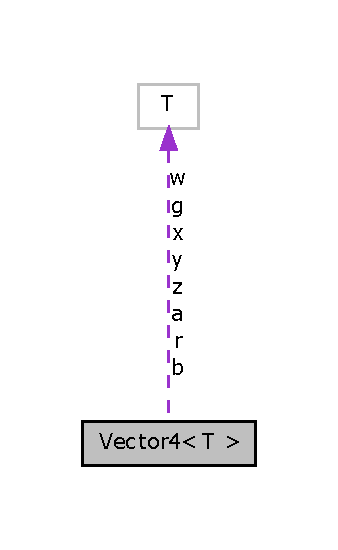
\includegraphics[width=162pt]{class_vector4__coll__graph}
\end{center}
\end{figure}
\subsection*{Public Member Functions}
\begin{DoxyCompactItemize}
\item 
\hyperlink{class_vector4_afdef97d94e5697622b5322637028accf}{Vector4} ()
\begin{DoxyCompactList}\small\item\em Creates and sets to (0,0,0,0). \item\end{DoxyCompactList}\item 
\hyperlink{class_vector4_a6a51b14dfcb4b1bb4b0252f76e602ec8}{Vector4} (T nx, T ny, T nz, T nw)
\begin{DoxyCompactList}\small\item\em Creates and sets to (x,y,z,z). \item\end{DoxyCompactList}\item 
\hyperlink{class_vector4_ae20ddb27878b88964f059495b7311f35}{Vector4} (const \hyperlink{class_vector4}{Vector4}$<$ T $>$ \&src)
\begin{DoxyCompactList}\small\item\em Copy constructor. \item\end{DoxyCompactList}\item 
{\footnotesize template$<$class FromT $>$ }\\\hyperlink{class_vector4_afedec40c43f916ee0951d98c41676a0f}{Vector4} (const \hyperlink{class_vector4}{Vector4}$<$ FromT $>$ \&src)
\begin{DoxyCompactList}\small\item\em Copy casting constructor. \item\end{DoxyCompactList}\item 
\hyperlink{class_vector4}{Vector4}$<$ T $>$ \hyperlink{class_vector4_ace35647d296fb7b9d59083f2a4a7fa7a}{operator=} (const \hyperlink{class_vector4}{Vector4}$<$ T $>$ \&rhs)
\begin{DoxyCompactList}\small\item\em Copy operator. \item\end{DoxyCompactList}\item 
{\footnotesize template$<$class FromT $>$ }\\\hyperlink{class_vector4}{Vector4}$<$ T $>$ \hyperlink{class_vector4_a11f1097f1ff61938d79344f9cd28aad2}{operator=} (const \hyperlink{class_vector4}{Vector4}$<$ FromT $>$ \&rhs)
\begin{DoxyCompactList}\small\item\em Copy casting operator. \item\end{DoxyCompactList}\item 
T \& \hyperlink{class_vector4_a992debdc2a8aee9ba1bcc9bb763a1270}{operator\mbox{[}$\,$\mbox{]}} (int n)
\begin{DoxyCompactList}\small\item\em Array access operator. \item\end{DoxyCompactList}\item 
const T \& \hyperlink{class_vector4_a6ae2a5a65474cb93edc7aceac761850c}{operator\mbox{[}$\,$\mbox{]}} (int n) const 
\begin{DoxyCompactList}\small\item\em Array access operator. \item\end{DoxyCompactList}\item 
\hyperlink{class_vector4}{Vector4}$<$ T $>$ \hyperlink{class_vector4_a80a688fb0462045dd222a0b565477824}{operator+} (const \hyperlink{class_vector4}{Vector4}$<$ T $>$ \&rhs) const 
\begin{DoxyCompactList}\small\item\em Addition operator. \item\end{DoxyCompactList}\item 
\hyperlink{class_vector4}{Vector4}$<$ T $>$ \hyperlink{class_vector4_a46dae2fe0b182172dbc5940ce54329a1}{operator-\/} (const \hyperlink{class_vector4}{Vector4}$<$ T $>$ \&rhs) const 
\begin{DoxyCompactList}\small\item\em Subtraction operator. \item\end{DoxyCompactList}\item 
\hyperlink{class_vector4}{Vector4}$<$ T $>$ \hyperlink{class_vector4_a86f22a427d874dc481b949ed761f9896}{operator$\ast$} (const \hyperlink{class_vector4}{Vector4}$<$ T $>$ rhs) const 
\begin{DoxyCompactList}\small\item\em Multiplication operator. \item\end{DoxyCompactList}\item 
\hyperlink{class_vector4}{Vector4}$<$ T $>$ \hyperlink{class_vector4_ae71f14523d070c119854f1df4c5ee084}{operator/} (const \hyperlink{class_vector4}{Vector4}$<$ T $>$ \&rhs) const 
\begin{DoxyCompactList}\small\item\em Division operator. \item\end{DoxyCompactList}\item 
\hyperlink{class_vector4}{Vector4}$<$ T $>$ \& \hyperlink{class_vector4_abfa5fdfbc2f9569e467e05dd2ecaab26}{operator+=} (const \hyperlink{class_vector4}{Vector4}$<$ T $>$ \&rhs)
\begin{DoxyCompactList}\small\item\em Addition operator. \item\end{DoxyCompactList}\item 
\hyperlink{class_vector4}{Vector4}$<$ T $>$ \& \hyperlink{class_vector4_ad5cfb4045ea0305610179c6bae648520}{operator-\/=} (const \hyperlink{class_vector4}{Vector4}$<$ T $>$ \&rhs)
\begin{DoxyCompactList}\small\item\em Subtraction operator. \item\end{DoxyCompactList}\item 
\hyperlink{class_vector4}{Vector4}$<$ T $>$ \& \hyperlink{class_vector4_a3f5db01486e5265e137a112113cb6cf5}{operator$\ast$=} (const \hyperlink{class_vector4}{Vector4}$<$ T $>$ \&rhs)
\begin{DoxyCompactList}\small\item\em Multiplication operator. \item\end{DoxyCompactList}\item 
\hyperlink{class_vector4}{Vector4}$<$ T $>$ \& \hyperlink{class_vector4_a1dc992e52cfbd78bc502c644dc0521fe}{operator/=} (const \hyperlink{class_vector4}{Vector4}$<$ T $>$ \&rhs)
\begin{DoxyCompactList}\small\item\em Division operator. \item\end{DoxyCompactList}\item 
bool \hyperlink{class_vector4_a2e8f2ec10e407b1f3e731b62c03f8225}{operator==} (const \hyperlink{class_vector4}{Vector4}$<$ T $>$ \&rhs) const 
\begin{DoxyCompactList}\small\item\em Equality test operator. \item\end{DoxyCompactList}\item 
bool \hyperlink{class_vector4_ac31d726332dd8505246ca2360c60300d}{operator!=} (const \hyperlink{class_vector4}{Vector4}$<$ T $>$ \&rhs) const 
\begin{DoxyCompactList}\small\item\em Inequality test operator. \item\end{DoxyCompactList}\item 
\hyperlink{class_vector4}{Vector4}$<$ T $>$ \hyperlink{class_vector4_a7bc7d332788658a92b32694969b4d9e3}{operator-\/} () const 
\begin{DoxyCompactList}\small\item\em Unary negate operator. \item\end{DoxyCompactList}\item 
\hyperlink{class_vector4}{Vector4}$<$ T $>$ \hyperlink{class_vector4_a5004bc94b91923c985e23077cfc937a7}{operator+} (T rhs) const 
\begin{DoxyCompactList}\small\item\em Addition operator. \item\end{DoxyCompactList}\item 
\hyperlink{class_vector4}{Vector4}$<$ T $>$ \hyperlink{class_vector4_addd6c83bcdadd34c0038aae76138aebc}{operator-\/} (T rhs) const 
\begin{DoxyCompactList}\small\item\em Subtraction operator. \item\end{DoxyCompactList}\item 
\hyperlink{class_vector4}{Vector4}$<$ T $>$ \hyperlink{class_vector4_a98e56cc3ef735884b8f70e287ff2ed68}{operator$\ast$} (T rhs) const 
\begin{DoxyCompactList}\small\item\em Multiplication operator. \item\end{DoxyCompactList}\item 
\hyperlink{class_vector4}{Vector4}$<$ T $>$ \hyperlink{class_vector4_a512f5d096b767bcbe1618f01d5a2bebf}{operator/} (T rhs) const 
\begin{DoxyCompactList}\small\item\em Division operator. \item\end{DoxyCompactList}\item 
\hyperlink{class_vector4}{Vector4}$<$ T $>$ \& \hyperlink{class_vector4_a7d465ec9eaffaa3308c4a6c64f2ded8f}{operator+=} (T rhs)
\begin{DoxyCompactList}\small\item\em Addition operator. \item\end{DoxyCompactList}\item 
\hyperlink{class_vector4}{Vector4}$<$ T $>$ \& \hyperlink{class_vector4_a908ced73c807151645080dc7bb9f8516}{operator-\/=} (T rhs)
\begin{DoxyCompactList}\small\item\em Subtraction operator. \item\end{DoxyCompactList}\item 
\hyperlink{class_vector4}{Vector4}$<$ T $>$ \& \hyperlink{class_vector4_a1caac7a97dae951da9039049c93db73f}{operator$\ast$=} (T rhs)
\begin{DoxyCompactList}\small\item\em Multiplication operator. \item\end{DoxyCompactList}\item 
\hyperlink{class_vector4}{Vector4}$<$ T $>$ \& \hyperlink{class_vector4_a2355ed974eac90e81de045dbf522b433}{operator/=} (T rhs)
\begin{DoxyCompactList}\small\item\em Division operator. \item\end{DoxyCompactList}\item 
T \hyperlink{class_vector4_a2242e63f194ec1a46efaae9417f3593c}{length} () const 
\begin{DoxyCompactList}\small\item\em Get length of vector. \item\end{DoxyCompactList}\item 
void \hyperlink{class_vector4_a854ae5d3ecf13efd5251a1e32c43f1b3}{normalize} ()
\begin{DoxyCompactList}\small\item\em Normalize vector. \item\end{DoxyCompactList}\item 
T \hyperlink{class_vector4_a32ac452a5ba86aaf90a3d75709990f0c}{lengthSq} () const 
\begin{DoxyCompactList}\small\item\em Return square of length. \item\end{DoxyCompactList}\item 
\hyperlink{class_vector4}{Vector4}$<$ T $>$ \hyperlink{class_vector4_a59a2b76485334331aa3a2759f3ff45b0}{lerp} (T fact, const \hyperlink{class_vector4}{Vector4}$<$ T $>$ \&\hyperlink{class_vector4_add0f79fe4a8f6d4e1d2aadb2f0c9bbdd}{r}) const 
\begin{DoxyCompactList}\small\item\em Linear interpolation of two vectors. \item\end{DoxyCompactList}\item 
\hyperlink{class_vector4_ac7f1f6e3b48b7878434200d7f2ff035c}{operator T $\ast$} ()
\begin{DoxyCompactList}\small\item\em Conversion to pointer operator. \item\end{DoxyCompactList}\item 
\hyperlink{class_vector4_a6bd576e3ee44ba853b2c8f854a237b2e}{operator const T $\ast$} () const 
\begin{DoxyCompactList}\small\item\em Conversion to pointer operator. \item\end{DoxyCompactList}\item 
std::string \hyperlink{class_vector4_af3ca83cdb1ee34545c18707232dfbc3d}{toString} () const 
\begin{DoxyCompactList}\small\item\em Gets string representation. \item\end{DoxyCompactList}\end{DoxyCompactItemize}
\subsection*{Public Attributes}
\begin{DoxyCompactItemize}
\item 
\begin{tabbing}
xx\=xx\=xx\=xx\=xx\=xx\=xx\=xx\=xx\=\kill
union \{\\
\>T \hyperlink{class_vector4_add0f79fe4a8f6d4e1d2aadb2f0c9bbdd}{r}\\
\>\>{\em First element of vector, alias for R-\/coordinate. }\\
\>T \hyperlink{class_vector4_a2cedf20d2f695a4f0254681b13311ac9}{x}\\
\}; \\

\end{tabbing}\item 
\begin{tabbing}
xx\=xx\=xx\=xx\=xx\=xx\=xx\=xx\=xx\=\kill
union \{\\
\>T \hyperlink{class_vector4_acd9cbf0e72286a325f50793cab3d94e0}{g}\\
\>\>{\em Second element of vector, alias for G-\/coordinate. }\\
\>T \hyperlink{class_vector4_aad001ba27515dc2dcb921e9c83596520}{y}\\
\>\>{\em Second element of vector, alias for Y-\/coordinate. }\\
\}; \\

\end{tabbing}\item 
\begin{tabbing}
xx\=xx\=xx\=xx\=xx\=xx\=xx\=xx\=xx\=\kill
union \{\\
\>T \hyperlink{class_vector4_a147df940f8e570124eb54226be07f28b}{b}\\
\>\>{\em Third element of vector, alias for B-\/coordinate. }\\
\>T \hyperlink{class_vector4_a5a7a1452d661e0b24e4b04c4dbff8ae7}{z}\\
\>\>{\em Third element of vector, alias for Z-\/coordinate. }\\
\}; \\

\end{tabbing}\item 
\begin{tabbing}
xx\=xx\=xx\=xx\=xx\=xx\=xx\=xx\=xx\=\kill
union \{\\
\>T \hyperlink{class_vector4_a32a0b541c80b0eb5c2c08634b7ab4e3b}{a}\\
\>\>{\em Fourth element of vector, alias for A-\/coordinate. }\\
\>T \hyperlink{class_vector4_a83daff43fa2b88b4e76474f4b9a45276}{w}\\
\>\>{\em First element of vector, alias for W-\/coordinate. }\\
\}; \\

\end{tabbing}\end{DoxyCompactItemize}
\subsection*{Friends}
\begin{DoxyCompactItemize}
\item 
std::ostream \& \hyperlink{class_vector4_acaeb205c81fccf7c59d96e13f1af1a21}{operator$<$$<$} (std::ostream \&lhs, const \hyperlink{class_vector4}{Vector4}$<$ T $>$ \&rhs)
\begin{DoxyCompactList}\small\item\em Output to stream operator. \item\end{DoxyCompactList}\end{DoxyCompactItemize}


\subsection{Detailed Description}
\subsubsection*{template$<$class T$>$ class Vector4$<$ T $>$}

Class for four dimensional vector. There are four ways of accessing vector components. Let's have {\ttfamily Vector4f v}, you can either: 
\begin{DoxyItemize}
\item access as position in projective space (x,y,z,w) --- {\ttfamily v.x = v.y = v.z = v.w = 1;} 
\item access as texture coordinate (s,t,u,v) --- {\ttfamily v.s = v.t = v.u = v.v = 1;} 
\item access as color (r,g,b,a) --- {\ttfamily v.r = v.g = v.b = v.a = 1;} 
\item access via operator\mbox{[}\mbox{]} --- {\ttfamily v\mbox{[}0\mbox{]} = v\mbox{[}1\mbox{]} = v\mbox{[}2\mbox{]} = v\mbox{[}3\mbox{]} = 1;} 
\end{DoxyItemize}

\subsection{Constructor \& Destructor Documentation}
\hypertarget{class_vector4_afdef97d94e5697622b5322637028accf}{
\index{Vector4@{Vector4}!Vector4@{Vector4}}
\index{Vector4@{Vector4}!Vector4@{Vector4}}
\subsubsection[{Vector4}]{\setlength{\rightskip}{0pt plus 5cm}template$<$class T$>$ {\bf Vector4}$<$ T $>$::{\bf Vector4} (
\begin{DoxyParamCaption}
{}
\end{DoxyParamCaption}
)\hspace{0.3cm}{\ttfamily  \mbox{[}inline\mbox{]}}}}
\label{class_vector4_afdef97d94e5697622b5322637028accf}


Creates and sets to (0,0,0,0). 

\hypertarget{class_vector4_a6a51b14dfcb4b1bb4b0252f76e602ec8}{
\index{Vector4@{Vector4}!Vector4@{Vector4}}
\index{Vector4@{Vector4}!Vector4@{Vector4}}
\subsubsection[{Vector4}]{\setlength{\rightskip}{0pt plus 5cm}template$<$class T$>$ {\bf Vector4}$<$ T $>$::{\bf Vector4} (
\begin{DoxyParamCaption}
\item[{T}]{ nx, }
\item[{T}]{ ny, }
\item[{T}]{ nz, }
\item[{T}]{ nw}
\end{DoxyParamCaption}
)\hspace{0.3cm}{\ttfamily  \mbox{[}inline\mbox{]}}}}
\label{class_vector4_a6a51b14dfcb4b1bb4b0252f76e602ec8}


Creates and sets to (x,y,z,z). 


\begin{DoxyParams}{Parameters}
\item[{\em nx}]initial x-\/coordinate value (R) \item[{\em ny}]initial y-\/coordinate value (G) \item[{\em nz}]initial z-\/coordinate value (B) \item[{\em nw}]initial w-\/coordinate value (Alpha) \end{DoxyParams}
\hypertarget{class_vector4_ae20ddb27878b88964f059495b7311f35}{
\index{Vector4@{Vector4}!Vector4@{Vector4}}
\index{Vector4@{Vector4}!Vector4@{Vector4}}
\subsubsection[{Vector4}]{\setlength{\rightskip}{0pt plus 5cm}template$<$class T$>$ {\bf Vector4}$<$ T $>$::{\bf Vector4} (
\begin{DoxyParamCaption}
\item[{const {\bf Vector4}$<$ T $>$ \&}]{ src}
\end{DoxyParamCaption}
)\hspace{0.3cm}{\ttfamily  \mbox{[}inline\mbox{]}}}}
\label{class_vector4_ae20ddb27878b88964f059495b7311f35}


Copy constructor. 


\begin{DoxyParams}{Parameters}
\item[{\em src}]Source of data for new created \hyperlink{class_vector4}{Vector4} instance. \end{DoxyParams}
\hypertarget{class_vector4_afedec40c43f916ee0951d98c41676a0f}{
\index{Vector4@{Vector4}!Vector4@{Vector4}}
\index{Vector4@{Vector4}!Vector4@{Vector4}}
\subsubsection[{Vector4}]{\setlength{\rightskip}{0pt plus 5cm}template$<$class T$>$ template$<$class FromT $>$ {\bf Vector4}$<$ T $>$::{\bf Vector4} (
\begin{DoxyParamCaption}
\item[{const {\bf Vector4}$<$ FromT $>$ \&}]{ src}
\end{DoxyParamCaption}
)\hspace{0.3cm}{\ttfamily  \mbox{[}inline\mbox{]}}}}
\label{class_vector4_afedec40c43f916ee0951d98c41676a0f}


Copy casting constructor. 


\begin{DoxyParams}{Parameters}
\item[{\em src}]Source of data for new created \hyperlink{class_vector4}{Vector4} instance. \end{DoxyParams}


\subsection{Member Function Documentation}
\hypertarget{class_vector4_a2242e63f194ec1a46efaae9417f3593c}{
\index{Vector4@{Vector4}!length@{length}}
\index{length@{length}!Vector4@{Vector4}}
\subsubsection[{length}]{\setlength{\rightskip}{0pt plus 5cm}template$<$class T$>$ T {\bf Vector4}$<$ T $>$::length (
\begin{DoxyParamCaption}
{}
\end{DoxyParamCaption}
) const\hspace{0.3cm}{\ttfamily  \mbox{[}inline\mbox{]}}}}
\label{class_vector4_a2242e63f194ec1a46efaae9417f3593c}


Get length of vector. 

\begin{DoxyReturn}{Returns}
lenght of vector 
\end{DoxyReturn}
\hypertarget{class_vector4_a32ac452a5ba86aaf90a3d75709990f0c}{
\index{Vector4@{Vector4}!lengthSq@{lengthSq}}
\index{lengthSq@{lengthSq}!Vector4@{Vector4}}
\subsubsection[{lengthSq}]{\setlength{\rightskip}{0pt plus 5cm}template$<$class T$>$ T {\bf Vector4}$<$ T $>$::lengthSq (
\begin{DoxyParamCaption}
{}
\end{DoxyParamCaption}
) const\hspace{0.3cm}{\ttfamily  \mbox{[}inline\mbox{]}}}}
\label{class_vector4_a32ac452a5ba86aaf90a3d75709990f0c}


Return square of length. 

\begin{DoxyReturn}{Returns}
length $^\wedge$ 2 
\end{DoxyReturn}
\begin{DoxyNote}{Note}
This method is faster then \hyperlink{class_vector4_a2242e63f194ec1a46efaae9417f3593c}{length()}. For comparison of length of two vector can be used just this value, instead of more expensive \hyperlink{class_vector4_a2242e63f194ec1a46efaae9417f3593c}{length()} method. 
\end{DoxyNote}
\hypertarget{class_vector4_a59a2b76485334331aa3a2759f3ff45b0}{
\index{Vector4@{Vector4}!lerp@{lerp}}
\index{lerp@{lerp}!Vector4@{Vector4}}
\subsubsection[{lerp}]{\setlength{\rightskip}{0pt plus 5cm}template$<$class T$>$ {\bf Vector4}$<$T$>$ {\bf Vector4}$<$ T $>$::lerp (
\begin{DoxyParamCaption}
\item[{T}]{ fact, }
\item[{const {\bf Vector4}$<$ T $>$ \&}]{ r}
\end{DoxyParamCaption}
) const\hspace{0.3cm}{\ttfamily  \mbox{[}inline\mbox{]}}}}
\label{class_vector4_a59a2b76485334331aa3a2759f3ff45b0}


Linear interpolation of two vectors. 


\begin{DoxyParams}{Parameters}
\item[{\em fact}]Factor of interpolation. For translation from position of this vector to vector r, values of factor goes from 0.0 to 1.0. \item[{\em r}]Second Vector for interpolation \end{DoxyParams}
\begin{DoxyNote}{Note}
However values of fact parameter are reasonable only in interval \mbox{[}0.0 , 1.0\mbox{]}, you can pass also values outside of this interval and you can get result (extrapolation?) 
\end{DoxyNote}
\hypertarget{class_vector4_a854ae5d3ecf13efd5251a1e32c43f1b3}{
\index{Vector4@{Vector4}!normalize@{normalize}}
\index{normalize@{normalize}!Vector4@{Vector4}}
\subsubsection[{normalize}]{\setlength{\rightskip}{0pt plus 5cm}template$<$class T$>$ void {\bf Vector4}$<$ T $>$::normalize (
\begin{DoxyParamCaption}
{}
\end{DoxyParamCaption}
)\hspace{0.3cm}{\ttfamily  \mbox{[}inline\mbox{]}}}}
\label{class_vector4_a854ae5d3ecf13efd5251a1e32c43f1b3}


Normalize vector. 

\hypertarget{class_vector4_a6bd576e3ee44ba853b2c8f854a237b2e}{
\index{Vector4@{Vector4}!operator const T $\ast$@{operator const T $\ast$}}
\index{operator const T $\ast$@{operator const T $\ast$}!Vector4@{Vector4}}
\subsubsection[{operator const T $\ast$}]{\setlength{\rightskip}{0pt plus 5cm}template$<$class T$>$ {\bf Vector4}$<$ T $>$::operator const T $\ast$ (
\begin{DoxyParamCaption}
{}
\end{DoxyParamCaption}
) const\hspace{0.3cm}{\ttfamily  \mbox{[}inline\mbox{]}}}}
\label{class_vector4_a6bd576e3ee44ba853b2c8f854a237b2e}


Conversion to pointer operator. 

\begin{DoxyReturn}{Returns}
Constant Pointer to internally stored (in management of class Vector4$<$T$>$) used for passing Vector4$<$T$>$ values to gl$\ast$4\mbox{[}fd\mbox{]} functions. 
\end{DoxyReturn}
\hypertarget{class_vector4_ac7f1f6e3b48b7878434200d7f2ff035c}{
\index{Vector4@{Vector4}!operator T $\ast$@{operator T $\ast$}}
\index{operator T $\ast$@{operator T $\ast$}!Vector4@{Vector4}}
\subsubsection[{operator T $\ast$}]{\setlength{\rightskip}{0pt plus 5cm}template$<$class T$>$ {\bf Vector4}$<$ T $>$::operator T $\ast$ (
\begin{DoxyParamCaption}
{}
\end{DoxyParamCaption}
)\hspace{0.3cm}{\ttfamily  \mbox{[}inline\mbox{]}}}}
\label{class_vector4_ac7f1f6e3b48b7878434200d7f2ff035c}


Conversion to pointer operator. 

\begin{DoxyReturn}{Returns}
Pointer to internally stored (in management of class Vector4$<$T$>$) used for passing Vector4$<$T$>$ values to gl$\ast$4\mbox{[}fd\mbox{]} functions. 
\end{DoxyReturn}
\hypertarget{class_vector4_ac31d726332dd8505246ca2360c60300d}{
\index{Vector4@{Vector4}!operator!=@{operator!=}}
\index{operator!=@{operator!=}!Vector4@{Vector4}}
\subsubsection[{operator!=}]{\setlength{\rightskip}{0pt plus 5cm}template$<$class T$>$ bool {\bf Vector4}$<$ T $>$::operator!= (
\begin{DoxyParamCaption}
\item[{const {\bf Vector4}$<$ T $>$ \&}]{ rhs}
\end{DoxyParamCaption}
) const\hspace{0.3cm}{\ttfamily  \mbox{[}inline\mbox{]}}}}
\label{class_vector4_ac31d726332dd8505246ca2360c60300d}


Inequality test operator. 


\begin{DoxyParams}{Parameters}
\item[{\em rhs}]Right hand side argument of binary operator. \end{DoxyParams}
\begin{DoxyReturn}{Returns}
not (lhs == rhs) :-\/P 
\end{DoxyReturn}
\hypertarget{class_vector4_a98e56cc3ef735884b8f70e287ff2ed68}{
\index{Vector4@{Vector4}!operator$\ast$@{operator$\ast$}}
\index{operator$\ast$@{operator$\ast$}!Vector4@{Vector4}}
\subsubsection[{operator$\ast$}]{\setlength{\rightskip}{0pt plus 5cm}template$<$class T$>$ {\bf Vector4}$<$T$>$ {\bf Vector4}$<$ T $>$::operator$\ast$ (
\begin{DoxyParamCaption}
\item[{T}]{ rhs}
\end{DoxyParamCaption}
) const\hspace{0.3cm}{\ttfamily  \mbox{[}inline\mbox{]}}}}
\label{class_vector4_a98e56cc3ef735884b8f70e287ff2ed68}


Multiplication operator. 


\begin{DoxyParams}{Parameters}
\item[{\em rhs}]Right hand side argument of binary operator. \end{DoxyParams}
\hypertarget{class_vector4_a86f22a427d874dc481b949ed761f9896}{
\index{Vector4@{Vector4}!operator$\ast$@{operator$\ast$}}
\index{operator$\ast$@{operator$\ast$}!Vector4@{Vector4}}
\subsubsection[{operator$\ast$}]{\setlength{\rightskip}{0pt plus 5cm}template$<$class T$>$ {\bf Vector4}$<$T$>$ {\bf Vector4}$<$ T $>$::operator$\ast$ (
\begin{DoxyParamCaption}
\item[{const {\bf Vector4}$<$ T $>$}]{ rhs}
\end{DoxyParamCaption}
) const\hspace{0.3cm}{\ttfamily  \mbox{[}inline\mbox{]}}}}
\label{class_vector4_a86f22a427d874dc481b949ed761f9896}


Multiplication operator. 


\begin{DoxyParams}{Parameters}
\item[{\em rhs}]Right hand side argument of binary operator. \end{DoxyParams}
\hypertarget{class_vector4_a3f5db01486e5265e137a112113cb6cf5}{
\index{Vector4@{Vector4}!operator$\ast$=@{operator$\ast$=}}
\index{operator$\ast$=@{operator$\ast$=}!Vector4@{Vector4}}
\subsubsection[{operator$\ast$=}]{\setlength{\rightskip}{0pt plus 5cm}template$<$class T$>$ {\bf Vector4}$<$T$>$\& {\bf Vector4}$<$ T $>$::operator$\ast$= (
\begin{DoxyParamCaption}
\item[{const {\bf Vector4}$<$ T $>$ \&}]{ rhs}
\end{DoxyParamCaption}
)\hspace{0.3cm}{\ttfamily  \mbox{[}inline\mbox{]}}}}
\label{class_vector4_a3f5db01486e5265e137a112113cb6cf5}


Multiplication operator. 


\begin{DoxyParams}{Parameters}
\item[{\em rhs}]Right hand side argument of binary operator. \end{DoxyParams}
\hypertarget{class_vector4_a1caac7a97dae951da9039049c93db73f}{
\index{Vector4@{Vector4}!operator$\ast$=@{operator$\ast$=}}
\index{operator$\ast$=@{operator$\ast$=}!Vector4@{Vector4}}
\subsubsection[{operator$\ast$=}]{\setlength{\rightskip}{0pt plus 5cm}template$<$class T$>$ {\bf Vector4}$<$T$>$\& {\bf Vector4}$<$ T $>$::operator$\ast$= (
\begin{DoxyParamCaption}
\item[{T}]{ rhs}
\end{DoxyParamCaption}
)\hspace{0.3cm}{\ttfamily  \mbox{[}inline\mbox{]}}}}
\label{class_vector4_a1caac7a97dae951da9039049c93db73f}


Multiplication operator. 


\begin{DoxyParams}{Parameters}
\item[{\em rhs}]Right hand side argument of binary operator. \end{DoxyParams}
\hypertarget{class_vector4_a5004bc94b91923c985e23077cfc937a7}{
\index{Vector4@{Vector4}!operator+@{operator+}}
\index{operator+@{operator+}!Vector4@{Vector4}}
\subsubsection[{operator+}]{\setlength{\rightskip}{0pt plus 5cm}template$<$class T$>$ {\bf Vector4}$<$T$>$ {\bf Vector4}$<$ T $>$::operator+ (
\begin{DoxyParamCaption}
\item[{T}]{ rhs}
\end{DoxyParamCaption}
) const\hspace{0.3cm}{\ttfamily  \mbox{[}inline\mbox{]}}}}
\label{class_vector4_a5004bc94b91923c985e23077cfc937a7}


Addition operator. 


\begin{DoxyParams}{Parameters}
\item[{\em rhs}]Right hand side argument of binary operator. \end{DoxyParams}
\hypertarget{class_vector4_a80a688fb0462045dd222a0b565477824}{
\index{Vector4@{Vector4}!operator+@{operator+}}
\index{operator+@{operator+}!Vector4@{Vector4}}
\subsubsection[{operator+}]{\setlength{\rightskip}{0pt plus 5cm}template$<$class T$>$ {\bf Vector4}$<$T$>$ {\bf Vector4}$<$ T $>$::operator+ (
\begin{DoxyParamCaption}
\item[{const {\bf Vector4}$<$ T $>$ \&}]{ rhs}
\end{DoxyParamCaption}
) const\hspace{0.3cm}{\ttfamily  \mbox{[}inline\mbox{]}}}}
\label{class_vector4_a80a688fb0462045dd222a0b565477824}


Addition operator. 


\begin{DoxyParams}{Parameters}
\item[{\em rhs}]Right hand side argument of binary operator. \end{DoxyParams}
\hypertarget{class_vector4_a7d465ec9eaffaa3308c4a6c64f2ded8f}{
\index{Vector4@{Vector4}!operator+=@{operator+=}}
\index{operator+=@{operator+=}!Vector4@{Vector4}}
\subsubsection[{operator+=}]{\setlength{\rightskip}{0pt plus 5cm}template$<$class T$>$ {\bf Vector4}$<$T$>$\& {\bf Vector4}$<$ T $>$::operator+= (
\begin{DoxyParamCaption}
\item[{T}]{ rhs}
\end{DoxyParamCaption}
)\hspace{0.3cm}{\ttfamily  \mbox{[}inline\mbox{]}}}}
\label{class_vector4_a7d465ec9eaffaa3308c4a6c64f2ded8f}


Addition operator. 


\begin{DoxyParams}{Parameters}
\item[{\em rhs}]Right hand side argument of binary operator. \end{DoxyParams}
\hypertarget{class_vector4_abfa5fdfbc2f9569e467e05dd2ecaab26}{
\index{Vector4@{Vector4}!operator+=@{operator+=}}
\index{operator+=@{operator+=}!Vector4@{Vector4}}
\subsubsection[{operator+=}]{\setlength{\rightskip}{0pt plus 5cm}template$<$class T$>$ {\bf Vector4}$<$T$>$\& {\bf Vector4}$<$ T $>$::operator+= (
\begin{DoxyParamCaption}
\item[{const {\bf Vector4}$<$ T $>$ \&}]{ rhs}
\end{DoxyParamCaption}
)\hspace{0.3cm}{\ttfamily  \mbox{[}inline\mbox{]}}}}
\label{class_vector4_abfa5fdfbc2f9569e467e05dd2ecaab26}


Addition operator. 


\begin{DoxyParams}{Parameters}
\item[{\em rhs}]Right hand side argument of binary operator. \end{DoxyParams}
\hypertarget{class_vector4_addd6c83bcdadd34c0038aae76138aebc}{
\index{Vector4@{Vector4}!operator-\/@{operator-\/}}
\index{operator-\/@{operator-\/}!Vector4@{Vector4}}
\subsubsection[{operator-\/}]{\setlength{\rightskip}{0pt plus 5cm}template$<$class T$>$ {\bf Vector4}$<$T$>$ {\bf Vector4}$<$ T $>$::operator-\/ (
\begin{DoxyParamCaption}
\item[{T}]{ rhs}
\end{DoxyParamCaption}
) const\hspace{0.3cm}{\ttfamily  \mbox{[}inline\mbox{]}}}}
\label{class_vector4_addd6c83bcdadd34c0038aae76138aebc}


Subtraction operator. 


\begin{DoxyParams}{Parameters}
\item[{\em rhs}]Right hand side argument of binary operator. \end{DoxyParams}
\hypertarget{class_vector4_a46dae2fe0b182172dbc5940ce54329a1}{
\index{Vector4@{Vector4}!operator-\/@{operator-\/}}
\index{operator-\/@{operator-\/}!Vector4@{Vector4}}
\subsubsection[{operator-\/}]{\setlength{\rightskip}{0pt plus 5cm}template$<$class T$>$ {\bf Vector4}$<$T$>$ {\bf Vector4}$<$ T $>$::operator-\/ (
\begin{DoxyParamCaption}
\item[{const {\bf Vector4}$<$ T $>$ \&}]{ rhs}
\end{DoxyParamCaption}
) const\hspace{0.3cm}{\ttfamily  \mbox{[}inline\mbox{]}}}}
\label{class_vector4_a46dae2fe0b182172dbc5940ce54329a1}


Subtraction operator. 


\begin{DoxyParams}{Parameters}
\item[{\em rhs}]Right hand side argument of binary operator. \end{DoxyParams}
\hypertarget{class_vector4_a7bc7d332788658a92b32694969b4d9e3}{
\index{Vector4@{Vector4}!operator-\/@{operator-\/}}
\index{operator-\/@{operator-\/}!Vector4@{Vector4}}
\subsubsection[{operator-\/}]{\setlength{\rightskip}{0pt plus 5cm}template$<$class T$>$ {\bf Vector4}$<$T$>$ {\bf Vector4}$<$ T $>$::operator-\/ (
\begin{DoxyParamCaption}
{}
\end{DoxyParamCaption}
) const\hspace{0.3cm}{\ttfamily  \mbox{[}inline\mbox{]}}}}
\label{class_vector4_a7bc7d332788658a92b32694969b4d9e3}


Unary negate operator. 

\begin{DoxyReturn}{Returns}
negated vector 
\end{DoxyReturn}
\hypertarget{class_vector4_a908ced73c807151645080dc7bb9f8516}{
\index{Vector4@{Vector4}!operator-\/=@{operator-\/=}}
\index{operator-\/=@{operator-\/=}!Vector4@{Vector4}}
\subsubsection[{operator-\/=}]{\setlength{\rightskip}{0pt plus 5cm}template$<$class T$>$ {\bf Vector4}$<$T$>$\& {\bf Vector4}$<$ T $>$::operator-\/= (
\begin{DoxyParamCaption}
\item[{T}]{ rhs}
\end{DoxyParamCaption}
)\hspace{0.3cm}{\ttfamily  \mbox{[}inline\mbox{]}}}}
\label{class_vector4_a908ced73c807151645080dc7bb9f8516}


Subtraction operator. 


\begin{DoxyParams}{Parameters}
\item[{\em rhs}]Right hand side argument of binary operator. \end{DoxyParams}
\hypertarget{class_vector4_ad5cfb4045ea0305610179c6bae648520}{
\index{Vector4@{Vector4}!operator-\/=@{operator-\/=}}
\index{operator-\/=@{operator-\/=}!Vector4@{Vector4}}
\subsubsection[{operator-\/=}]{\setlength{\rightskip}{0pt plus 5cm}template$<$class T$>$ {\bf Vector4}$<$T$>$\& {\bf Vector4}$<$ T $>$::operator-\/= (
\begin{DoxyParamCaption}
\item[{const {\bf Vector4}$<$ T $>$ \&}]{ rhs}
\end{DoxyParamCaption}
)\hspace{0.3cm}{\ttfamily  \mbox{[}inline\mbox{]}}}}
\label{class_vector4_ad5cfb4045ea0305610179c6bae648520}


Subtraction operator. 


\begin{DoxyParams}{Parameters}
\item[{\em rhs}]Right hand side argument of binary operator. \end{DoxyParams}
\hypertarget{class_vector4_ae71f14523d070c119854f1df4c5ee084}{
\index{Vector4@{Vector4}!operator/@{operator/}}
\index{operator/@{operator/}!Vector4@{Vector4}}
\subsubsection[{operator/}]{\setlength{\rightskip}{0pt plus 5cm}template$<$class T$>$ {\bf Vector4}$<$T$>$ {\bf Vector4}$<$ T $>$::operator/ (
\begin{DoxyParamCaption}
\item[{const {\bf Vector4}$<$ T $>$ \&}]{ rhs}
\end{DoxyParamCaption}
) const\hspace{0.3cm}{\ttfamily  \mbox{[}inline\mbox{]}}}}
\label{class_vector4_ae71f14523d070c119854f1df4c5ee084}


Division operator. 


\begin{DoxyParams}{Parameters}
\item[{\em rhs}]Right hand side argument of binary operator. \end{DoxyParams}
\hypertarget{class_vector4_a512f5d096b767bcbe1618f01d5a2bebf}{
\index{Vector4@{Vector4}!operator/@{operator/}}
\index{operator/@{operator/}!Vector4@{Vector4}}
\subsubsection[{operator/}]{\setlength{\rightskip}{0pt plus 5cm}template$<$class T$>$ {\bf Vector4}$<$T$>$ {\bf Vector4}$<$ T $>$::operator/ (
\begin{DoxyParamCaption}
\item[{T}]{ rhs}
\end{DoxyParamCaption}
) const\hspace{0.3cm}{\ttfamily  \mbox{[}inline\mbox{]}}}}
\label{class_vector4_a512f5d096b767bcbe1618f01d5a2bebf}


Division operator. 


\begin{DoxyParams}{Parameters}
\item[{\em rhs}]Right hand side argument of binary operator. \end{DoxyParams}
\hypertarget{class_vector4_a2355ed974eac90e81de045dbf522b433}{
\index{Vector4@{Vector4}!operator/=@{operator/=}}
\index{operator/=@{operator/=}!Vector4@{Vector4}}
\subsubsection[{operator/=}]{\setlength{\rightskip}{0pt plus 5cm}template$<$class T$>$ {\bf Vector4}$<$T$>$\& {\bf Vector4}$<$ T $>$::operator/= (
\begin{DoxyParamCaption}
\item[{T}]{ rhs}
\end{DoxyParamCaption}
)\hspace{0.3cm}{\ttfamily  \mbox{[}inline\mbox{]}}}}
\label{class_vector4_a2355ed974eac90e81de045dbf522b433}


Division operator. 


\begin{DoxyParams}{Parameters}
\item[{\em rhs}]Right hand side argument of binary operator. \end{DoxyParams}
\hypertarget{class_vector4_a1dc992e52cfbd78bc502c644dc0521fe}{
\index{Vector4@{Vector4}!operator/=@{operator/=}}
\index{operator/=@{operator/=}!Vector4@{Vector4}}
\subsubsection[{operator/=}]{\setlength{\rightskip}{0pt plus 5cm}template$<$class T$>$ {\bf Vector4}$<$T$>$\& {\bf Vector4}$<$ T $>$::operator/= (
\begin{DoxyParamCaption}
\item[{const {\bf Vector4}$<$ T $>$ \&}]{ rhs}
\end{DoxyParamCaption}
)\hspace{0.3cm}{\ttfamily  \mbox{[}inline\mbox{]}}}}
\label{class_vector4_a1dc992e52cfbd78bc502c644dc0521fe}


Division operator. 


\begin{DoxyParams}{Parameters}
\item[{\em rhs}]Right hand side argument of binary operator. \end{DoxyParams}
\hypertarget{class_vector4_a11f1097f1ff61938d79344f9cd28aad2}{
\index{Vector4@{Vector4}!operator=@{operator=}}
\index{operator=@{operator=}!Vector4@{Vector4}}
\subsubsection[{operator=}]{\setlength{\rightskip}{0pt plus 5cm}template$<$class T$>$ template$<$class FromT $>$ {\bf Vector4}$<$T$>$ {\bf Vector4}$<$ T $>$::operator= (
\begin{DoxyParamCaption}
\item[{const {\bf Vector4}$<$ FromT $>$ \&}]{ rhs}
\end{DoxyParamCaption}
)\hspace{0.3cm}{\ttfamily  \mbox{[}inline\mbox{]}}}}
\label{class_vector4_a11f1097f1ff61938d79344f9cd28aad2}


Copy casting operator. 


\begin{DoxyParams}{Parameters}
\item[{\em rhs}]Right hand side argument of binary operator. \end{DoxyParams}
\hypertarget{class_vector4_ace35647d296fb7b9d59083f2a4a7fa7a}{
\index{Vector4@{Vector4}!operator=@{operator=}}
\index{operator=@{operator=}!Vector4@{Vector4}}
\subsubsection[{operator=}]{\setlength{\rightskip}{0pt plus 5cm}template$<$class T$>$ {\bf Vector4}$<$T$>$ {\bf Vector4}$<$ T $>$::operator= (
\begin{DoxyParamCaption}
\item[{const {\bf Vector4}$<$ T $>$ \&}]{ rhs}
\end{DoxyParamCaption}
)\hspace{0.3cm}{\ttfamily  \mbox{[}inline\mbox{]}}}}
\label{class_vector4_ace35647d296fb7b9d59083f2a4a7fa7a}


Copy operator. 


\begin{DoxyParams}{Parameters}
\item[{\em rhs}]Right hand side argument of binary operator. \end{DoxyParams}
\hypertarget{class_vector4_a2e8f2ec10e407b1f3e731b62c03f8225}{
\index{Vector4@{Vector4}!operator==@{operator==}}
\index{operator==@{operator==}!Vector4@{Vector4}}
\subsubsection[{operator==}]{\setlength{\rightskip}{0pt plus 5cm}template$<$class T$>$ bool {\bf Vector4}$<$ T $>$::operator== (
\begin{DoxyParamCaption}
\item[{const {\bf Vector4}$<$ T $>$ \&}]{ rhs}
\end{DoxyParamCaption}
) const\hspace{0.3cm}{\ttfamily  \mbox{[}inline\mbox{]}}}}
\label{class_vector4_a2e8f2ec10e407b1f3e731b62c03f8225}


Equality test operator. 


\begin{DoxyParams}{Parameters}
\item[{\em rhs}]Right hand side argument of binary operator. \end{DoxyParams}
\begin{DoxyNote}{Note}
Test of equality is based of threshold EPSILON value. To be two values equal, must satisfy this condition $|$ lhs.x -\/ rhs.y $|$ $<$ EPSILON, same for y-\/coordinate, z-\/coordinate, and w-\/coordinate. 
\end{DoxyNote}
\hypertarget{class_vector4_a992debdc2a8aee9ba1bcc9bb763a1270}{
\index{Vector4@{Vector4}!operator\mbox{[}\mbox{]}@{operator[]}}
\index{operator\mbox{[}\mbox{]}@{operator[]}!Vector4@{Vector4}}
\subsubsection[{operator[]}]{\setlength{\rightskip}{0pt plus 5cm}template$<$class T$>$ T\& {\bf Vector4}$<$ T $>$::operator\mbox{[}$\,$\mbox{]} (
\begin{DoxyParamCaption}
\item[{int}]{ n}
\end{DoxyParamCaption}
)\hspace{0.3cm}{\ttfamily  \mbox{[}inline\mbox{]}}}}
\label{class_vector4_a992debdc2a8aee9ba1bcc9bb763a1270}


Array access operator. 


\begin{DoxyParams}{Parameters}
\item[{\em n}]Array index \end{DoxyParams}
\begin{DoxyReturn}{Returns}
For n = 0, reference to x coordinate, n = 1 reference to y coordinate, n = 2 reference to z, else reference to w coordinate. 
\end{DoxyReturn}
\hypertarget{class_vector4_a6ae2a5a65474cb93edc7aceac761850c}{
\index{Vector4@{Vector4}!operator\mbox{[}\mbox{]}@{operator[]}}
\index{operator\mbox{[}\mbox{]}@{operator[]}!Vector4@{Vector4}}
\subsubsection[{operator[]}]{\setlength{\rightskip}{0pt plus 5cm}template$<$class T$>$ const T\& {\bf Vector4}$<$ T $>$::operator\mbox{[}$\,$\mbox{]} (
\begin{DoxyParamCaption}
\item[{int}]{ n}
\end{DoxyParamCaption}
) const\hspace{0.3cm}{\ttfamily  \mbox{[}inline\mbox{]}}}}
\label{class_vector4_a6ae2a5a65474cb93edc7aceac761850c}


Array access operator. 


\begin{DoxyParams}{Parameters}
\item[{\em n}]Array index \end{DoxyParams}
\begin{DoxyReturn}{Returns}
For n = 0, reference to x coordinate, n = 1 reference to y coordinate, n = 2 reference to z, else reference to w coordinate. 
\end{DoxyReturn}
\hypertarget{class_vector4_af3ca83cdb1ee34545c18707232dfbc3d}{
\index{Vector4@{Vector4}!toString@{toString}}
\index{toString@{toString}!Vector4@{Vector4}}
\subsubsection[{toString}]{\setlength{\rightskip}{0pt plus 5cm}template$<$class T$>$ std::string {\bf Vector4}$<$ T $>$::toString (
\begin{DoxyParamCaption}
{}
\end{DoxyParamCaption}
) const\hspace{0.3cm}{\ttfamily  \mbox{[}inline\mbox{]}}}}
\label{class_vector4_af3ca83cdb1ee34545c18707232dfbc3d}


Gets string representation. 



\subsection{Friends And Related Function Documentation}
\hypertarget{class_vector4_acaeb205c81fccf7c59d96e13f1af1a21}{
\index{Vector4@{Vector4}!operator$<$$<$@{operator$<$$<$}}
\index{operator$<$$<$@{operator$<$$<$}!Vector4@{Vector4}}
\subsubsection[{operator$<$$<$}]{\setlength{\rightskip}{0pt plus 5cm}template$<$class T$>$ std::ostream\& operator$<$$<$ (
\begin{DoxyParamCaption}
\item[{std::ostream \&}]{ lhs, }
\item[{const {\bf Vector4}$<$ T $>$ \&}]{ rhs}
\end{DoxyParamCaption}
)\hspace{0.3cm}{\ttfamily  \mbox{[}friend\mbox{]}}}}
\label{class_vector4_acaeb205c81fccf7c59d96e13f1af1a21}


Output to stream operator. 


\begin{DoxyParams}{Parameters}
\item[{\em lhs}]Left hand side argument of operator (commonly ostream instance). \item[{\em rhs}]Right hand side argument of operator. \end{DoxyParams}
\begin{DoxyReturn}{Returns}
Left hand side argument -\/ the ostream object passed to operator. 
\end{DoxyReturn}


\subsection{Member Data Documentation}
\hypertarget{class_vector4_a687a777e033b4aeb36745512a285ab15}{
\subsubsection[{"@11}]{\setlength{\rightskip}{0pt plus 5cm}union \{ ... \} }}
\label{class_vector4_a687a777e033b4aeb36745512a285ab15}
\hypertarget{class_vector4_a7c73c2be47abaf5d0e688cc2e09d2a74}{
\subsubsection[{"@13}]{\setlength{\rightskip}{0pt plus 5cm}union \{ ... \} }}
\label{class_vector4_a7c73c2be47abaf5d0e688cc2e09d2a74}
\hypertarget{class_vector4_a7bed48fe8a1f4f4f603ee8124ace6374}{
\subsubsection[{"@15}]{\setlength{\rightskip}{0pt plus 5cm}union \{ ... \} }}
\label{class_vector4_a7bed48fe8a1f4f4f603ee8124ace6374}
\hypertarget{class_vector4_ad6edebc0c1fcc9d21489d1a12fa47ccf}{
\subsubsection[{"@17}]{\setlength{\rightskip}{0pt plus 5cm}union \{ ... \} }}
\label{class_vector4_ad6edebc0c1fcc9d21489d1a12fa47ccf}
\hypertarget{class_vector4_a32a0b541c80b0eb5c2c08634b7ab4e3b}{
\index{Vector4@{Vector4}!a@{a}}
\index{a@{a}!Vector4@{Vector4}}
\subsubsection[{a}]{\setlength{\rightskip}{0pt plus 5cm}template$<$class T$>$ T {\bf Vector4}$<$ T $>$::{\bf a}}}
\label{class_vector4_a32a0b541c80b0eb5c2c08634b7ab4e3b}


Fourth element of vector, alias for A-\/coordinate. 

For color notation. This represnt aplha chanell \hypertarget{class_vector4_a147df940f8e570124eb54226be07f28b}{
\index{Vector4@{Vector4}!b@{b}}
\index{b@{b}!Vector4@{Vector4}}
\subsubsection[{b}]{\setlength{\rightskip}{0pt plus 5cm}template$<$class T$>$ T {\bf Vector4}$<$ T $>$::{\bf b}}}
\label{class_vector4_a147df940f8e570124eb54226be07f28b}


Third element of vector, alias for B-\/coordinate. 

For color notation. \hypertarget{class_vector4_acd9cbf0e72286a325f50793cab3d94e0}{
\index{Vector4@{Vector4}!g@{g}}
\index{g@{g}!Vector4@{Vector4}}
\subsubsection[{g}]{\setlength{\rightskip}{0pt plus 5cm}template$<$class T$>$ T {\bf Vector4}$<$ T $>$::{\bf g}}}
\label{class_vector4_acd9cbf0e72286a325f50793cab3d94e0}


Second element of vector, alias for G-\/coordinate. 

For color notation. \hypertarget{class_vector4_add0f79fe4a8f6d4e1d2aadb2f0c9bbdd}{
\index{Vector4@{Vector4}!r@{r}}
\index{r@{r}!Vector4@{Vector4}}
\subsubsection[{r}]{\setlength{\rightskip}{0pt plus 5cm}template$<$class T$>$ T {\bf Vector4}$<$ T $>$::{\bf r}}}
\label{class_vector4_add0f79fe4a8f6d4e1d2aadb2f0c9bbdd}


First element of vector, alias for R-\/coordinate. 

For color notation. First element of vector, alias for X-\/coordinate. \hypertarget{class_vector4_a83daff43fa2b88b4e76474f4b9a45276}{
\index{Vector4@{Vector4}!w@{w}}
\index{w@{w}!Vector4@{Vector4}}
\subsubsection[{w}]{\setlength{\rightskip}{0pt plus 5cm}template$<$class T$>$ T {\bf Vector4}$<$ T $>$::{\bf w}}}
\label{class_vector4_a83daff43fa2b88b4e76474f4b9a45276}


First element of vector, alias for W-\/coordinate. 

\begin{DoxyNote}{Note}
For vectors (such as normals) should be set to 0.0 For vertices should be set to 1.0 
\end{DoxyNote}
\hypertarget{class_vector4_a2cedf20d2f695a4f0254681b13311ac9}{
\index{Vector4@{Vector4}!x@{x}}
\index{x@{x}!Vector4@{Vector4}}
\subsubsection[{x}]{\setlength{\rightskip}{0pt plus 5cm}template$<$class T$>$ T {\bf Vector4}$<$ T $>$::{\bf x}}}
\label{class_vector4_a2cedf20d2f695a4f0254681b13311ac9}
\hypertarget{class_vector4_aad001ba27515dc2dcb921e9c83596520}{
\index{Vector4@{Vector4}!y@{y}}
\index{y@{y}!Vector4@{Vector4}}
\subsubsection[{y}]{\setlength{\rightskip}{0pt plus 5cm}template$<$class T$>$ T {\bf Vector4}$<$ T $>$::{\bf y}}}
\label{class_vector4_aad001ba27515dc2dcb921e9c83596520}


Second element of vector, alias for Y-\/coordinate. 

\hypertarget{class_vector4_a5a7a1452d661e0b24e4b04c4dbff8ae7}{
\index{Vector4@{Vector4}!z@{z}}
\index{z@{z}!Vector4@{Vector4}}
\subsubsection[{z}]{\setlength{\rightskip}{0pt plus 5cm}template$<$class T$>$ T {\bf Vector4}$<$ T $>$::{\bf z}}}
\label{class_vector4_a5a7a1452d661e0b24e4b04c4dbff8ae7}


Third element of vector, alias for Z-\/coordinate. 



The documentation for this class was generated from the following file:\begin{DoxyCompactItemize}
\item 
src/\hyperlink{vmath_8h}{vmath.h}\end{DoxyCompactItemize}

\chapter{File Documentation}
\hypertarget{vmath_8cpp}{
\section{src/vmath.cpp File Reference}
\label{vmath_8cpp}\index{src/vmath.cpp@{src/vmath.cpp}}
}
{\ttfamily \#include \char`\"{}vmath.h\char`\"{}}\par
Include dependency graph for vmath.cpp:\nopagebreak
\begin{figure}[H]
\begin{center}
\leavevmode
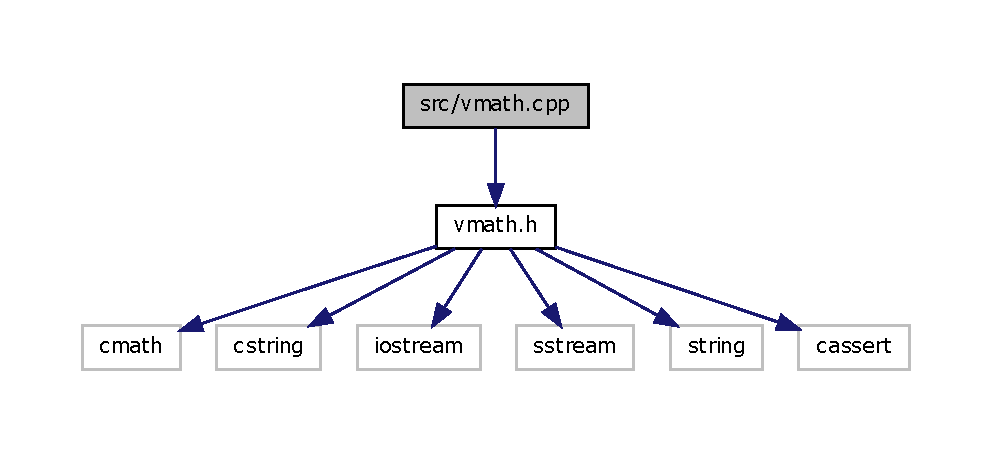
\includegraphics[width=400pt]{vmath_8cpp__incl}
\end{center}
\end{figure}

\hypertarget{vmath_8h}{
\section{src/vmath.h File Reference}
\label{vmath_8h}\index{src/vmath.h@{src/vmath.h}}
}
{\ttfamily \#include $<$cmath$>$}\par
{\ttfamily \#include $<$cstring$>$}\par
{\ttfamily \#include $<$iostream$>$}\par
{\ttfamily \#include $<$sstream$>$}\par
{\ttfamily \#include $<$string$>$}\par
{\ttfamily \#include $<$cassert$>$}\par
Include dependency graph for vmath.h:
\nopagebreak
\begin{figure}[H]
\begin{center}
\leavevmode
\includegraphics[width=400pt]{vmath_8h__incl}
\end{center}
\end{figure}
This graph shows which files directly or indirectly include this file:
\nopagebreak
\begin{figure}[H]
\begin{center}
\leavevmode
\includegraphics[width=168pt]{vmath_8h__dep__incl}
\end{center}
\end{figure}
\subsection*{Classes}
\begin{DoxyCompactItemize}
\item 
class \hyperlink{class_vector2}{Vector2$<$ T $>$}
\begin{DoxyCompactList}\small\item\em Class for two dimensional vector. \item\end{DoxyCompactList}\item 
class \hyperlink{class_vector3}{Vector3$<$ T $>$}
\begin{DoxyCompactList}\small\item\em Class for three dimensional vector. \item\end{DoxyCompactList}\item 
class \hyperlink{class_vector4}{Vector4$<$ T $>$}
\begin{DoxyCompactList}\small\item\em Class for four dimensional vector. \item\end{DoxyCompactList}\item 
class \hyperlink{class_matrix3}{Matrix3$<$ T $>$}
\begin{DoxyCompactList}\small\item\em Class for matrix 3x3. \item\end{DoxyCompactList}\item 
class \hyperlink{class_matrix4}{Matrix4$<$ T $>$}
\begin{DoxyCompactList}\small\item\em Class for matrix 4x4. \item\end{DoxyCompactList}\item 
class \hyperlink{class_quaternion}{Quaternion$<$ T $>$}
\begin{DoxyCompactList}\small\item\em \hyperlink{class_quaternion}{Quaternion} class implementing some quaternion algebra operations. \item\end{DoxyCompactList}\end{DoxyCompactItemize}
\subsection*{Defines}
\begin{DoxyCompactItemize}
\item 
\#define \hyperlink{vmath_8h_ae71449b1cc6e6250b91f539153a7a0d3}{M\_\-PI}~3.14159265358979323846
\item 
\#define \hyperlink{vmath_8h_a2b4f9c3a8b58ecc8e9a6cda26417ba00}{DEG2RAD}(x)~((x $\ast$ M\_\-PI) / 180.0)
\item 
\#define \hyperlink{vmath_8h_a002b2f4894492820fe708b1b7e7c5e70}{EPSILON}~\hyperlink{vmath_8h_ac29df3dcbefa1ce189e5990bde994025}{epsilon}
\end{DoxyCompactItemize}
\subsection*{Typedefs}
\begin{DoxyCompactItemize}
\item 
typedef class \hyperlink{class_vector2}{Vector2}$<$ float $>$ \hyperlink{vmath_8h_ad3bb0ec940392ad40277673a25d7d99e}{Vector2f}
\begin{DoxyCompactList}\small\item\em Two dimensional Vector of floats. \item\end{DoxyCompactList}\item 
typedef class \hyperlink{class_vector2}{Vector2}$<$ double $>$ \hyperlink{vmath_8h_ae98713ced2b133072ea124b46df07b26}{Vector2d}
\begin{DoxyCompactList}\small\item\em Two dimensional Vector of doubles. \item\end{DoxyCompactList}\item 
typedef class \hyperlink{class_vector2}{Vector2}$<$ int $>$ \hyperlink{vmath_8h_a69ae23b6f5cac98abb0d42436001307c}{Vector2i}
\begin{DoxyCompactList}\small\item\em Two dimensional Vector of ints. \item\end{DoxyCompactList}\item 
typedef \hyperlink{class_vector3}{Vector3}$<$ float $>$ \hyperlink{vmath_8h_af345ad77ba5e240c7ab72b4b2077e754}{Vector3f}
\begin{DoxyCompactList}\small\item\em Three dimensional Vector of floats. \item\end{DoxyCompactList}\item 
typedef \hyperlink{class_vector3}{Vector3}$<$ double $>$ \hyperlink{vmath_8h_a1f05093f5ee1a9ecdd54476792e4c206}{Vector3d}
\begin{DoxyCompactList}\small\item\em Three dimensional Vector of doubles. \item\end{DoxyCompactList}\item 
typedef \hyperlink{class_vector3}{Vector3}$<$ int $>$ \hyperlink{vmath_8h_a6951accbbf6263a1ac8019bf718ae31c}{Vector3i}
\begin{DoxyCompactList}\small\item\em Three dimensional Vector of ints. \item\end{DoxyCompactList}\item 
typedef \hyperlink{class_vector4}{Vector4}$<$ float $>$ \hyperlink{vmath_8h_a2e950d4be17eed0a7d6f24353b04c8f5}{Vector4f}
\begin{DoxyCompactList}\small\item\em Three dimensional Vector of floats. \item\end{DoxyCompactList}\item 
typedef \hyperlink{class_vector4}{Vector4}$<$ double $>$ \hyperlink{vmath_8h_ad0b18996675624521849970fa6bf09c3}{Vector4d}
\begin{DoxyCompactList}\small\item\em Three dimensional Vector of doubles. \item\end{DoxyCompactList}\item 
typedef \hyperlink{class_vector4}{Vector4}$<$ int $>$ \hyperlink{vmath_8h_a270bbc7b96b874207992bb5456218a48}{Vector4i}
\begin{DoxyCompactList}\small\item\em Three dimensional Vector of ints. \item\end{DoxyCompactList}\item 
typedef \hyperlink{class_matrix3}{Matrix3}$<$ float $>$ \hyperlink{vmath_8h_ae5a673b3d27428dc13b294596cc53a5d}{Matrix3f}
\begin{DoxyCompactList}\small\item\em Matrix 3x3 of floats. \item\end{DoxyCompactList}\item 
typedef \hyperlink{class_matrix3}{Matrix3}$<$ double $>$ \hyperlink{vmath_8h_a86e6f4c9798f85f6b09c74b4b60d2376}{Matrix3d}
\begin{DoxyCompactList}\small\item\em Matrix 3x3 of doubles. \item\end{DoxyCompactList}\item 
typedef \hyperlink{class_matrix3}{Matrix3}$<$ int $>$ \hyperlink{vmath_8h_a968bc4736fac5af106094c63c24ac6ca}{Matrix3i}
\begin{DoxyCompactList}\small\item\em Matrix 3x3 of int. \item\end{DoxyCompactList}\item 
typedef \hyperlink{class_matrix4}{Matrix4}$<$ float $>$ \hyperlink{vmath_8h_a5b7721ab7216c91a40538beaa9e6ee1f}{Matrix4f}
\begin{DoxyCompactList}\small\item\em Matrix 4x4 of floats. \item\end{DoxyCompactList}\item 
typedef \hyperlink{class_matrix4}{Matrix4}$<$ double $>$ \hyperlink{vmath_8h_afe7ea008ee9e656fb34621264a42e04a}{Matrix4d}
\begin{DoxyCompactList}\small\item\em Matrix 4x4 of doubles. \item\end{DoxyCompactList}\item 
typedef \hyperlink{class_matrix4}{Matrix4}$<$ int $>$ \hyperlink{vmath_8h_a21a14a0a49d405a9014fa9e11af3425e}{Matrix4i}
\begin{DoxyCompactList}\small\item\em Matrix 4x4 of int. \item\end{DoxyCompactList}\item 
typedef \hyperlink{class_quaternion}{Quaternion}$<$ float $>$ \hyperlink{vmath_8h_a00cefb008ef0f3f16cf6e001b4f62b8c}{Quatf}
\item 
typedef \hyperlink{class_quaternion}{Quaternion}$<$ double $>$ \hyperlink{vmath_8h_a37eb0465222e99d52254e9822b999480}{Quatd}
\end{DoxyCompactItemize}
\subsection*{Variables}
\begin{DoxyCompactItemize}
\item 
const double \hyperlink{vmath_8h_ac29df3dcbefa1ce189e5990bde994025}{epsilon} = 4.37114e-\/05
\end{DoxyCompactItemize}


\subsection{Define Documentation}
\hypertarget{vmath_8h_a2b4f9c3a8b58ecc8e9a6cda26417ba00}{
\index{vmath.h@{vmath.h}!DEG2RAD@{DEG2RAD}}
\index{DEG2RAD@{DEG2RAD}!vmath.h@{vmath.h}}
\subsubsection[{DEG2RAD}]{\setlength{\rightskip}{0pt plus 5cm}\#define DEG2RAD(
\begin{DoxyParamCaption}
\item[{}]{x}
\end{DoxyParamCaption}
)~((x $\ast$ M\_\-PI) / 180.0)}}
\label{vmath_8h_a2b4f9c3a8b58ecc8e9a6cda26417ba00}
\hypertarget{vmath_8h_a002b2f4894492820fe708b1b7e7c5e70}{
\index{vmath.h@{vmath.h}!EPSILON@{EPSILON}}
\index{EPSILON@{EPSILON}!vmath.h@{vmath.h}}
\subsubsection[{EPSILON}]{\setlength{\rightskip}{0pt plus 5cm}\#define EPSILON~{\bf epsilon}}}
\label{vmath_8h_a002b2f4894492820fe708b1b7e7c5e70}
\hypertarget{vmath_8h_ae71449b1cc6e6250b91f539153a7a0d3}{
\index{vmath.h@{vmath.h}!M\_\-PI@{M\_\-PI}}
\index{M\_\-PI@{M\_\-PI}!vmath.h@{vmath.h}}
\subsubsection[{M\_\-PI}]{\setlength{\rightskip}{0pt plus 5cm}\#define M\_\-PI~3.14159265358979323846}}
\label{vmath_8h_ae71449b1cc6e6250b91f539153a7a0d3}


\subsection{Typedef Documentation}
\hypertarget{vmath_8h_a86e6f4c9798f85f6b09c74b4b60d2376}{
\index{vmath.h@{vmath.h}!Matrix3d@{Matrix3d}}
\index{Matrix3d@{Matrix3d}!vmath.h@{vmath.h}}
\subsubsection[{Matrix3d}]{\setlength{\rightskip}{0pt plus 5cm}typedef {\bf Matrix3}$<$double$>$ {\bf Matrix3d}}}
\label{vmath_8h_a86e6f4c9798f85f6b09c74b4b60d2376}


Matrix 3x3 of doubles. 

\hypertarget{vmath_8h_ae5a673b3d27428dc13b294596cc53a5d}{
\index{vmath.h@{vmath.h}!Matrix3f@{Matrix3f}}
\index{Matrix3f@{Matrix3f}!vmath.h@{vmath.h}}
\subsubsection[{Matrix3f}]{\setlength{\rightskip}{0pt plus 5cm}typedef {\bf Matrix3}$<$float$>$ {\bf Matrix3f}}}
\label{vmath_8h_ae5a673b3d27428dc13b294596cc53a5d}


Matrix 3x3 of floats. 

\hypertarget{vmath_8h_a968bc4736fac5af106094c63c24ac6ca}{
\index{vmath.h@{vmath.h}!Matrix3i@{Matrix3i}}
\index{Matrix3i@{Matrix3i}!vmath.h@{vmath.h}}
\subsubsection[{Matrix3i}]{\setlength{\rightskip}{0pt plus 5cm}typedef {\bf Matrix3}$<$int$>$ {\bf Matrix3i}}}
\label{vmath_8h_a968bc4736fac5af106094c63c24ac6ca}


Matrix 3x3 of int. 

\hypertarget{vmath_8h_afe7ea008ee9e656fb34621264a42e04a}{
\index{vmath.h@{vmath.h}!Matrix4d@{Matrix4d}}
\index{Matrix4d@{Matrix4d}!vmath.h@{vmath.h}}
\subsubsection[{Matrix4d}]{\setlength{\rightskip}{0pt plus 5cm}typedef {\bf Matrix4}$<$double$>$ {\bf Matrix4d}}}
\label{vmath_8h_afe7ea008ee9e656fb34621264a42e04a}


Matrix 4x4 of doubles. 

\hypertarget{vmath_8h_a5b7721ab7216c91a40538beaa9e6ee1f}{
\index{vmath.h@{vmath.h}!Matrix4f@{Matrix4f}}
\index{Matrix4f@{Matrix4f}!vmath.h@{vmath.h}}
\subsubsection[{Matrix4f}]{\setlength{\rightskip}{0pt plus 5cm}typedef {\bf Matrix4}$<$float$>$ {\bf Matrix4f}}}
\label{vmath_8h_a5b7721ab7216c91a40538beaa9e6ee1f}


Matrix 4x4 of floats. 

\hypertarget{vmath_8h_a21a14a0a49d405a9014fa9e11af3425e}{
\index{vmath.h@{vmath.h}!Matrix4i@{Matrix4i}}
\index{Matrix4i@{Matrix4i}!vmath.h@{vmath.h}}
\subsubsection[{Matrix4i}]{\setlength{\rightskip}{0pt plus 5cm}typedef {\bf Matrix4}$<$int$>$ {\bf Matrix4i}}}
\label{vmath_8h_a21a14a0a49d405a9014fa9e11af3425e}


Matrix 4x4 of int. 

\hypertarget{vmath_8h_a37eb0465222e99d52254e9822b999480}{
\index{vmath.h@{vmath.h}!Quatd@{Quatd}}
\index{Quatd@{Quatd}!vmath.h@{vmath.h}}
\subsubsection[{Quatd}]{\setlength{\rightskip}{0pt plus 5cm}typedef {\bf Quaternion}$<$double$>$ {\bf Quatd}}}
\label{vmath_8h_a37eb0465222e99d52254e9822b999480}
\hypertarget{vmath_8h_a00cefb008ef0f3f16cf6e001b4f62b8c}{
\index{vmath.h@{vmath.h}!Quatf@{Quatf}}
\index{Quatf@{Quatf}!vmath.h@{vmath.h}}
\subsubsection[{Quatf}]{\setlength{\rightskip}{0pt plus 5cm}typedef {\bf Quaternion}$<$float$>$ {\bf Quatf}}}
\label{vmath_8h_a00cefb008ef0f3f16cf6e001b4f62b8c}
\hypertarget{vmath_8h_ae98713ced2b133072ea124b46df07b26}{
\index{vmath.h@{vmath.h}!Vector2d@{Vector2d}}
\index{Vector2d@{Vector2d}!vmath.h@{vmath.h}}
\subsubsection[{Vector2d}]{\setlength{\rightskip}{0pt plus 5cm}typedef class {\bf Vector2}$<$ double $>$ {\bf Vector2d}}}
\label{vmath_8h_ae98713ced2b133072ea124b46df07b26}


Two dimensional Vector of doubles. 

\hypertarget{vmath_8h_ad3bb0ec940392ad40277673a25d7d99e}{
\index{vmath.h@{vmath.h}!Vector2f@{Vector2f}}
\index{Vector2f@{Vector2f}!vmath.h@{vmath.h}}
\subsubsection[{Vector2f}]{\setlength{\rightskip}{0pt plus 5cm}typedef class {\bf Vector2}$<$ float $>$ {\bf Vector2f}}}
\label{vmath_8h_ad3bb0ec940392ad40277673a25d7d99e}


Two dimensional Vector of floats. 

\hypertarget{vmath_8h_a69ae23b6f5cac98abb0d42436001307c}{
\index{vmath.h@{vmath.h}!Vector2i@{Vector2i}}
\index{Vector2i@{Vector2i}!vmath.h@{vmath.h}}
\subsubsection[{Vector2i}]{\setlength{\rightskip}{0pt plus 5cm}typedef class {\bf Vector2}$<$ int $>$ {\bf Vector2i}}}
\label{vmath_8h_a69ae23b6f5cac98abb0d42436001307c}


Two dimensional Vector of ints. 

\hypertarget{vmath_8h_a1f05093f5ee1a9ecdd54476792e4c206}{
\index{vmath.h@{vmath.h}!Vector3d@{Vector3d}}
\index{Vector3d@{Vector3d}!vmath.h@{vmath.h}}
\subsubsection[{Vector3d}]{\setlength{\rightskip}{0pt plus 5cm}typedef {\bf Vector3}$<$double$>$ {\bf Vector3d}}}
\label{vmath_8h_a1f05093f5ee1a9ecdd54476792e4c206}


Three dimensional Vector of doubles. 

\hypertarget{vmath_8h_af345ad77ba5e240c7ab72b4b2077e754}{
\index{vmath.h@{vmath.h}!Vector3f@{Vector3f}}
\index{Vector3f@{Vector3f}!vmath.h@{vmath.h}}
\subsubsection[{Vector3f}]{\setlength{\rightskip}{0pt plus 5cm}typedef {\bf Vector3}$<$float$>$ {\bf Vector3f}}}
\label{vmath_8h_af345ad77ba5e240c7ab72b4b2077e754}


Three dimensional Vector of floats. 

\hypertarget{vmath_8h_a6951accbbf6263a1ac8019bf718ae31c}{
\index{vmath.h@{vmath.h}!Vector3i@{Vector3i}}
\index{Vector3i@{Vector3i}!vmath.h@{vmath.h}}
\subsubsection[{Vector3i}]{\setlength{\rightskip}{0pt plus 5cm}typedef {\bf Vector3}$<$int$>$ {\bf Vector3i}}}
\label{vmath_8h_a6951accbbf6263a1ac8019bf718ae31c}


Three dimensional Vector of ints. 

\hypertarget{vmath_8h_ad0b18996675624521849970fa6bf09c3}{
\index{vmath.h@{vmath.h}!Vector4d@{Vector4d}}
\index{Vector4d@{Vector4d}!vmath.h@{vmath.h}}
\subsubsection[{Vector4d}]{\setlength{\rightskip}{0pt plus 5cm}typedef {\bf Vector4}$<$double$>$ {\bf Vector4d}}}
\label{vmath_8h_ad0b18996675624521849970fa6bf09c3}


Three dimensional Vector of doubles. 

\hypertarget{vmath_8h_a2e950d4be17eed0a7d6f24353b04c8f5}{
\index{vmath.h@{vmath.h}!Vector4f@{Vector4f}}
\index{Vector4f@{Vector4f}!vmath.h@{vmath.h}}
\subsubsection[{Vector4f}]{\setlength{\rightskip}{0pt plus 5cm}typedef {\bf Vector4}$<$float$>$ {\bf Vector4f}}}
\label{vmath_8h_a2e950d4be17eed0a7d6f24353b04c8f5}


Three dimensional Vector of floats. 

\hypertarget{vmath_8h_a270bbc7b96b874207992bb5456218a48}{
\index{vmath.h@{vmath.h}!Vector4i@{Vector4i}}
\index{Vector4i@{Vector4i}!vmath.h@{vmath.h}}
\subsubsection[{Vector4i}]{\setlength{\rightskip}{0pt plus 5cm}typedef {\bf Vector4}$<$int$>$ {\bf Vector4i}}}
\label{vmath_8h_a270bbc7b96b874207992bb5456218a48}


Three dimensional Vector of ints. 



\subsection{Variable Documentation}
\hypertarget{vmath_8h_ac29df3dcbefa1ce189e5990bde994025}{
\index{vmath.h@{vmath.h}!epsilon@{epsilon}}
\index{epsilon@{epsilon}!vmath.h@{vmath.h}}
\subsubsection[{epsilon}]{\setlength{\rightskip}{0pt plus 5cm}const double {\bf epsilon} = 4.37114e-\/05}}
\label{vmath_8h_ac29df3dcbefa1ce189e5990bde994025}

\printindex
\end{document}
